\PassOptionsToPackage{svgnames,dvipsnames,svgnames}{xcolor}

%for a more compact document, add the option openany to avoid
%starting all chapters on odd numbered pages
\documentclass[12pt]{cmuthesis}
%\usepackage[usenames,dvipsnames,svgnames]{xcolor}

% This is a template for a CMU thesis.  It is 18 pages without any content :-)
% The source for this is pulled from a variety of sources and people.
% Here's a partial list of people who may or may have not contributed:
%
%        bnoble   = Brian Noble
%        caruana  = Rich Caruana
%        colohan  = Chris Colohan
%        jab      = Justin Boyan
%        josullvn = Joseph O'Sullivan
%        jrs      = Jonathan Shewchuk
%        kosak    = Corey Kosak
%        mjz      = Matt Zekauskas (mattz@cs)
%        pdinda   = Peter Dinda
%        pfr      = Patrick Riley
%        dkoes = David Koes (me)

% My main contribution is putting everything into a single class files and small
% template since I prefer this to some complicated sprawling directory tree with
% makefiles.
\newcommand{\todolater}[1]{{\color{magenta} TODO (Later): #1}}
\newcommand{\todo}[1]{{\color{red} TODO: #1}}

% some useful packages
\usepackage{times}     % use times font for document
%\usepackage{lmodern}
\usepackage{newtxtt}
%\renewcommand{\ttdefault}{txtt} % use txtt for typewriter font
\usepackage{mathpazo}
\usepackage{mathpartir} % use package for inference rules
\usepackage{upgreek} % package for alternative greek letters (\uppi)
\usepackage{fullpage}
%\usepackage{graphicx}
\usepackage{amsmath,amssymb, amsthm}
\newtheorem{theorem}{Theorem}[chapter]
\newtheorem{lemma}[theorem]{Lemma}
\newtheorem{corollary}[theorem]{Corollary}
\newtheorem{definition}[theorem]{Definition}
\newtheorem{assumption}[theorem]{Assumption}
\newtheorem{condition}[theorem]{Condition}

\newenvironment{proof-sketch}{\noindent{\emph{Proof Sketch.}}}{\qed}

\usepackage{pfsteps}

\usepackage{ stmaryrd }
\usepackage[numbers,sort]{natbib}
\usepackage[colorlinks=true,allcolors=Green,backref,pageanchor=true,plainpages=false, pdfpagelabels, bookmarks,bookmarksnumbered,
pdfborder={0 0 0},  %removes outlines around hyper links in online display
]{hyperref}
\usepackage{subfigure}

% Approximately 1" margins, more space on binding side
%\usepackage[letterpaper,twoside,vscale=.8,hscale=.75,nomarginpar]{geometry}
%for general printing (not binding)
\usepackage[letterpaper,twoside,vscale=.8,hscale=.75,nomarginpar,hmarginratio=1:1]{geometry}

\usepackage{listings}
\lstset{tabsize=2, 
basicstyle=\ttfamily\fontsize{11pt}{1em}\selectfont, 
commentstyle=\itshape\ttfamily\color{gray}, 
stringstyle=\ttfamily\color{red},
mathescape=false,escapechar=\#,
numbers=left, numberstyle=\scriptsize\color{gray}\ttfamily, language=ML,moredelim=[il][\sffamily]{?},showspaces=false,showstringspaces=false,xleftmargin=15pt, morekeywords=[1]{tyfam,opfam,let,fn,val,def,casetype,objtype,metadata,of,*,datatype,new,toast,syntax,module,where,import,for,ana,syn,opcon,tycon,metasignature,metamodule,metasig,metamod,static,at,tycase,mod,macro,match,pattern,in,patterns,expressions},deletekeywords={double},classoffset=0,belowskip=\smallskipamount,
moredelim=**[is][\color{red}]{SSTR}{ESTR},
moredelim=**[is][\color{OliveGreen}]{SHTML}{EHTML},
moredelim=**[is][\color{purple}]{SCSS}{ECSS},
moredelim=**[is][\color{brown}]{SSQL}{ESQL},
moredelim=**[is][\color{orange}]{SCOLOR}{ECOLOR},
moredelim=**[is][\color{magenta}]{SPCT}{EPCT}, 
moredelim=**[is][\color{gray}]{SNAT}{ENAT}, 
moredelim=**[is][\color{blue}]{SURL}{EURL},
moredelim=**[is][\color{SeaGreen}]{SQT}{EQT},
moredelim=**[is][\color{Periwinkle}]{SGRM}{EGRM},
moredelim=**[is][\color{YellowGreen}]{SID}{EID},
moredelim=**[is][\color{Sepia}]{SUS}{EUS},
deletestring=[d]{"},
}
\lstloadlanguages{Java,VBScript,XML,HTML}
\let\li\lstinline

% http://tex.stackexchange.com/q/43526
% fix the apparently deliberate but undocumented behaviour of disabling escapes other than mathescape in TextStyle (used by \lstinline)
% there may be a good reason why this is disabled by default, so beware in case it causes any problems
\usepackage{etoolbox}
\makeatletter
\patchcmd{\lsthk@TextStyle}{\let\lst@DefEsc\@empty}{}{}{\errmessage{failed to patch}}
\makeatother

% Provides a draft mark at the top of the document. 
\draftstamp{\today}{DRAFT}


% I hate hyphenation.
\lefthyphenmin=5

% !TEX root = omar-thesis.tex
\newcommand{\dolla}{\texttt{\$}}  % used so I don't screw up syntax highlighting when using $ in an identifier inline

% \newcommand{\gheading}[1]{\multicolumn{3}{l}{\textbf{#1}}}

\newcommand{\elided}{{\color{gray}\cdots}}

% Calculi Names
\newcommand{\miniVerseUE}{\mathsf{miniVerse}_\textbf{UE}}
\newcommand{\miniVersePat}{\mathsf{miniVerse}_\textbf{U}}
\newcommand{\miniVerseParam}{\mathsf{miniVerse}_\mathbf{\forall}}
\newcommand{\miniVerseTSL}{\mathsf{miniVerse}_\textbf{TSL}}

% General abstract syntax
\newcommand{\aboppz}[2]{\texttt{#1}\texttt{[}#2\texttt{]}}
\newcommand{\abop}[2]{\texttt{#1}\texttt{(}#2\texttt{)}}
\newcommand{\abopi}[3]{\texttt{#1}[#2]\texttt{(}#3\texttt{)}}
\newcommand{\abopii}[4]{\texttt{#1}[#2][#3]\texttt{(}#4\texttt{)}}
\newcommand{\abopic}[4]{\texttt{#1}[#2]\texttt{\{}#3\texttt{\}(}#4\texttt{)}}
\newcommand{\abopp}[3]{\texttt{#1}\texttt{[}#2\texttt{](}#3\texttt{)}}
\newcommand{\abopc}[3]{\texttt{#1}\texttt{\{}#2\texttt{\}(}#3\texttt{)}}
\newcommand{\abopbc}[4]{\texttt{#1}\texttt{[}#2\texttt{]\{}#3\texttt{\}(}#4\texttt{)}}
\newcommand{\abopibc}[5]{\texttt{#1}[#2]\texttt{[}#3\texttt{]\{}#4\texttt{\}(}#5\texttt{)}}
\newcommand{\abopcc}[4]{\texttt{#1}\texttt{\{}#2\texttt{\}\{}#3\texttt{\}(}#4\texttt{)}}

% Types / candidate expansion types
\newcommand{\parr}[2]{#1 \rightharpoonup #2}
\newcommand{\aparr}[2]{\abop{parr}{#1; #2}}
\newcommand{\aceparr}[2]{\abop{ceparr}{#1; #2}}

\newcommand{\forallt}[2]{\forall #1.#2}
\newcommand{\aall}[2]{\abop{all}{#1.#2}}
\newcommand{\aceall}[2]{\abop{ceall}{#1.#2}}

\newcommand{\rect}[2]{\mu #1.#2}
\newcommand{\arec}[2]{\abop{rec}{#1.#2}}
\newcommand{\acerec}[2]{\abop{cerec}{#1.#2}}

\newcommand{\prodt}[1]{\langle #1 \rangle}
\newcommand{\aprod}[2]{\abopi{prod}{#1}{#2}}
\newcommand{\aceprod}[2]{\abopi{ceprod}{#1}{#2}}

\newcommand{\sumt}[1]{[#1]}
\newcommand{\asum}[2]{\abopi{sum}{#1}{#2}}
\newcommand{\acesum}[2]{\abopi{cesum}{#1}{#2}}

% Labels and maps
\newcommand{\labelset}{L}
\newcommand{\mapschema}[3]{\{#2 \hookrightarrow #1_{#2}\}_{#2 \in #3}}
\newcommand{\mapschemab}[4]{\{#3 \hookrightarrow #1_{#3}.#2_{#3}\}_{#3 \in #4}}
\newcommand{\finmap}[1]{#1}
\newcommand{\mapitem}[2]{#1 \hookrightarrow #2}
\newcommand{\lbltxt}[1]{\mathtt{#1}}

% sequences
\newcommand{\seqschema}[4]{\{#1_{#2}\}_{#3 \leq #2 \leq #4}}
\newcommand{\seqschemaX}[1]{\seqschema{#1}{i}{1}{n}}

% Expanded/Unexpanded/Candidate expressions
\newcommand{\lam}[3]{\lambda #1{:}#2.#3}
\newcommand{\aelam}[3]{\abopc{elam}{#1}{#2.#3}}
\newcommand{\aulam}[3]{\abopc{ulam}{#1}{#2.#3}}
\newcommand{\acelam}[3]{\abopc{celam}{#1}{#2.#3}}

\newcommand{\ap}[2]{#1(#2)}
\newcommand{\aeap}[2]{\abop{eap}{#1; #2}}
\newcommand{\auap}[2]{\abop{uap}{#1; #2}}
\newcommand{\aceap}[2]{\abop{ceap}{#1; #2}}

\newcommand{\Lam}[2]{\Lambda #1.#2}
\newcommand{\aetlam}[2]{\abop{etlam}{#1.#2}}
\newcommand{\autlam}[2]{\abop{utlam}{#1.#2}}
\newcommand{\acetlam}[2]{\abop{cetlam}{#1.#2}}

\newcommand{\App}[2]{#1\texttt{[}#2\texttt{]}}
\newcommand{\aetap}[2]{\abopc{etap}{#2}{#1}}
\newcommand{\autap}[2]{\abopc{utap}{#2}{#1}}
\newcommand{\acetap}[2]{\abopc{cetap}{#2}{#1}}

\newcommand{\fold}[1]{\texttt{fold}(#1)}
\newcommand{\aefold}[3]{\abopc{efold}{#1.#2}{#3}}
\newcommand{\aufold}[3]{\abopc{ufold}{#1.#2}{#3}}
\newcommand{\acefold}[3]{\abopc{cefold}{#1.#2}{#3}}

\newcommand{\unfold}[1]{\texttt{unfold}(#1)}
\newcommand{\aeunfold}[1]{\abop{eunfold}{#1}}
\newcommand{\auunfold}[1]{\abop{uunfold}{#1}}
\newcommand{\aceunfold}[1]{\abop{ceunfold}{#1}}

\newcommand{\tpl}[1]{\langle #1\rangle}
\newcommand{\aetpl}[2]{\abopi{etpl}{#1}{#2}}
\newcommand{\autpl}[2]{\abopi{utpl}{#1}{#2}}
\newcommand{\acetpl}[2]{\abopi{cetpl}{#1}{#2}}

\newcommand{\prj}[2]{#1 \cdot #2}
\newcommand{\aepr}[2]{\abopp{epr}{#1}{#2}}
\newcommand{\aupr}[2]{\abopp{upr}{#1}{#2}}
\newcommand{\acepr}[2]{\abopp{cepr}{#1}{#2}}

\newcommand{\inj}[2]{#1 \cdot #2}
\newcommand{\aein}[4]{\abopibc{ein}{#1}{#2}{#3}{#4}}
\newcommand{\auin}[4]{\abopibc{uin}{#1}{#2}{#3}{#4}}
\newcommand{\acein}[4]{\abopibc{cein}{#1}{#2}{#3}{#4}}

\newcommand{\caseof}[2]{\texttt{case}~#1~#2}
\newcommand{\aecase}[3]{\abopi{ecase}{#1}{#2; #3}}
\newcommand{\aucase}[3]{\abopi{ucase}{#1}{#2; #3}}
\newcommand{\acecase}[3]{\abopi{cecase}{#1}{#2; #3}}

% Expanded expressions
\newcommand{\etxt}[1]{e_\text{#1}}

\newcommand{\Uof}[1]{\mathcal{U}(#1)}
\newcommand{\VTypof}[1]{\mathcal{V}_\mathsf{Typ}(#1)}
\newcommand{\VExpof}[1]{\mathcal{V}_\mathsf{Exp}(#1)}
\newcommand{\rulemv}{R}

% Statics of miniVerseU expanded expressions
\newcommand{\istypeU}[2]{#1 \vdash #2~\mathsf{type}}
\newcommand{\isctxU}[2]{#1 \vdash #2~\mathsf{ctx}}
\newcommand{\hastypeU}[4]{#1~#2 \vdash #3 : #4}
\newcommand{\hastypeUC}[2]{\vdash #1 : #2}
\newcommand{\hastypeUCO}[3]{#1 \vdash #2 : #3}

\newcommand{\Dhyp}[1]{#1~\mathsf{type}}
\newcommand{\Dcons}[2]{{#1}\cup{#2}}
\newcommand{\Ghyp}[2]{#1 : #2}
\newcommand{\Gcons}[2]{{#1}\cup{#2}}
\newcommand{\Gconsi}[2]{\cup_{#1} #2}

% Dynamics of miniVerseU
\newcommand{\isvalU}[1]{#1~\mathsf{val}}
\newcommand{\stepsU}[2]{#1 \mapsto #2}
\newcommand{\multistepU}[2]{#1 \mapsto^{*} #2}
\newcommand{\evalU}[2]{#1 \Downarrow #2}

% Unexpanded expressions
\newcommand{\ue}{\hat{e}}
\newcommand{\uesyntax}[4]{\texttt{syntax}~#1~\texttt{at}~#2~\{#3\}~\texttt{in}~#4}
\newcommand{\audefuetsm}[4]{\abopcc{udefuetsm}{#1}{#2}{#3.#4}}
\newcommand{\utsmap}[2]{#1~\texttt{/}#2\texttt{/}}
\newcommand{\autsmap}[2]{\texttt{uapuetsm}[#1]\texttt{[}#2\texttt{]}}
\newcommand{\uet}[1]{\ue_\text{#1}}
\newcommand{\ueparse}{\uet{parse}}

% TSM expressions
\newcommand{\tsmv}{a}
\newcommand{\utsmdef}[2]{\texttt{syntax}~@~#1~\texttt{\{}#2\texttt{\}}}
\newcommand{\istsmU}[2]{#1 \vdash #2~\mathsf{tsm}}

\newcommand{\tBody}{\mathtt{Body}}
\newcommand{\tParseResultExp}{\mathtt{ParseResultExp}} 
\newcommand{\tCEExp}{\mathtt{CEExp}} % Typed expansion
\newcommand{\expandsU}[6]{#1~#2 \vdash_{#3} #4 \leadsto #5 : #6} % there's a multiline one in the document done manually
\newcommand{\expandsUX}[3]{\expandsU{\Delta}{\Gamma}{\Sigma}{#1}{#2}{#3}}
\newcommand{\expandsUC}[3]{\vdash #1 \leadsto #2 : #3}
\newcommand{\domof}[1]{\text{dom}(#1)}
\newcommand{\xuetsmdef}[2]{\abop{uetsm}{#1;\,#2}}
\newcommand{\xuetsmbnd}[3]{#1 \hookrightarrow \xuetsmdef{#2}{#3}}
\newcommand{\uetsmenv}[2]{#1 \vdash #2~\mathsf{ok}}
\newcommand{\encodeBody}[2]{#1 \downarrow #2}
\newcommand{\decodeBody}[2]{#1 \uparrow #2}
\newcommand{\ebody}{\etxt{body}}
\newcommand{\eparse}{\etxt{parse}}
\newcommand{\ecand}{\etxt{cand}}
\newcommand{\decodeCondE}[2]{#1 \uparrow_\mathsf{CEExp} #2}
\newcommand{\encodeCondE}[2]{#1 \downarrow_\mathsf{CEExp} #2}

% Candidate Expansions
\newcommand{\ce}{\grave{e}}
\newcommand{\ctau}{\grave{\tau}}

\newcommand{\splicedt}[2]{\texttt{spliced}\langle#1, #2\rangle}
\newcommand{\acesplicedt}[2]{\texttt{cesplicedt}[#1; #2]}
\newcommand{\splicede}[2]{\texttt{spliced}\langle#1, #2\rangle}
\newcommand{\acesplicede}[2]{\texttt{cesplicede}[#1; #2]}
\newcommand{\splicedp}[2]{\texttt{spliced}\langle#1, #2\rangle}
\newcommand{\acesplicedp}[2]{\texttt{cesplicedp}[#1; #2]}

\newcommand{\mtau}{\dot{\tau}}
\newcommand{\mtspliced}[1]{\texttt{spliced}(#1)}

% Candidate expansion validation
\newcommand{\cvalidT}[4]{#1\vdash^{#2} #3 \leadsto #4~\mathsf{type}}
\newcommand{\cvalidE}[6]{#1~#2\vdash^{#3} #4 \leadsto #5 : #6}
\newcommand{\cvalidEX}[3]{\cvalidE{\Delta}{\Gamma}{\escenev}{#1}{#2}{#3}}
\newcommand{\escenev}{\mathbbmss{E}}
\newcommand{\tscenev}{\mathbbmss{T}}
\newcommand{\esceneU}[4]{#1;\,#2;\,#3;\,#4}
\newcommand{\esceneUP}[5]{#1;\,#2;\,#3;\,#4;\,#5}
\newcommand{\tsceneU}[2]{#1;\,#2}
\newcommand{\tsceneUP}[2]{\tsceneU{#1}{#2}}
\newcommand{\tsfrom}[1]{\mathsf{ts}(#1)}
\newcommand{\parseTyp}[2]{\mathsf{parseTyp}(#1)=#2}
\newcommand{\parseUExp}[2]{\mathsf{parseUExp}(#1)=#2}
\newcommand{\bsubseq}[3]{\mathsf{subseq}(#1; #2; #3)}

\newcommand{\sizeof}[1]{\Vert #1 \Vert}

% Pattern matching
\newcommand{\matchwith}[2]{\texttt{match}~#1~#2}
\newcommand{\aematchwith}[3]{\abopi{ematch}{#1}{#2; #3}}
\newcommand{\aumatchwith}[3]{\abopi{umatch}{#1}{#2; #3}}
\newcommand{\acematchwith}[3]{\abopi{cematch}{#1}{#2; #3}}

\newcommand{\matchrule}[2]{#1 \Rightarrow #2}
\newcommand{\aematchrule}[4]{\abopii{erule}{#1}{#2}{#3.#4}}
\newcommand{\aumatchrule}[4]{\abopii{urule}{#1}{#2}{#3.#4}}
\newcommand{\acematchrule}[4]{\abopii{cerule}{#1}{#2}{#3.#4}}

\newcommand{\ruleType}[5]{#1~#2 \vdash #3 : #4 \Rightarrow #5}
\newcommand{\patType}[3]{#1 \Vdash #2 : #3}
\newcommand{\pctx}{\Omega}

\newcommand{\matchfail}[1]{#1~\mathsf{matchfail}}

\newcommand{\eR}{R}
\newcommand{\uR}{\hat{R}}
\newcommand{\cR}{\grave{R}}

\newcommand{\erv}{r}
\newcommand{\urv}{\hat{r}}
\newcommand{\crv}{\grave{r}}

\newcommand{\epv}{p}
\newcommand{\upv}{\hat{p}}
\newcommand{\cpv}{\grave{p}}

\newcommand{\wildp}{\_}
\newcommand{\aewildp}{\texttt{ewildp}}
\newcommand{\auwildp}{\texttt{uwildp}}
\newcommand{\acewildp}{\texttt{cewildp}}

\newcommand{\foldp}[1]{\abop{fold}{#1}}
\newcommand{\aefoldp}[1]{\abop{efoldp}{#1}}
\newcommand{\aufoldp}[1]{\abop{ufoldp}{#1}}
\newcommand{\acefoldp}[1]{\abop{cefoldp}{#1}}

\newcommand{\tplp}[1]{\langle #1 \rangle}
\newcommand{\aetplp}[2]{\abopi{etplp}{#1}{#2}}
\newcommand{\autplp}[2]{\abopi{utplp}{#1}{#2}}
\newcommand{\acetplp}[2]{\abopi{cetplp}{#1}{#2}}

\newcommand{\injp}[2]{#1 \cdot #2}
\newcommand{\aeinjp}[2]{\abopp{einp}{#1}{#2}}
\newcommand{\auinjp}[2]{\abopp{uinp}{#1}{#2}}
\newcommand{\aceinjp}[2]{\abopp{ceinp}{#1}{#2}}

\newcommand{\audefuptsm}[4]{\abopcc{udefuptsm}{#1}{#2}{#3.#4}}
\newcommand{\auapuptsm}[2]{\texttt{uapuptsm}[#1]\texttt{[}#2\texttt{]}}

\newcommand{\expandsUP}[7]{#1~#2 \vdash_{#3;\,#4} #5 \leadsto #6 : #7} % there's a multiline one in the document done manually
\newcommand{\expandsUPX}[3]{\expandsUP{\Delta}{\Gamma}{\Sigma}{\Phi}{#1}{#2}{#3}}

\newcommand{\ruleExpands}[8]{#1~#2 \vdash_{#3;\,#4} #5 \leadsto #6 : #7 \Rightarrow #8}
\newcommand{\patExpands}[5]{#1 \vdash_{#2} #3 \leadsto #4 : #5}
\newcommand{\xuptsmdef}[2]{\abop{uptsm}{#1;\,#2}}
\newcommand{\xuptsmbnd}[3]{#1 \hookrightarrow \xuptsmdef{#2}{#3}}
\newcommand{\uptsmenv}[2]{#1 \vdash #2~\mathsf{ok}}

\newcommand{\tParseResultPat}{\mathtt{ParseResultPat}} 
\newcommand{\tCEPat}{\mathtt{CEPat}} % Typed expansion

\newcommand{\decodeCEPat}[2]{#1 \uparrow_\mathsf{CEPat} #2}
\newcommand{\encodeCEPat}[2]{#1 \downarrow_\mathsf{CEPat} #2}

\newcommand{\cvalidP}[5]{\vdash^{#1;\,#2} #3 \leadsto #4 : #5}
\newcommand{\cvalidR}[7]{#1~#2 \vdash^{#3} #4 \leadsto #5 : #6 \Rightarrow #7}
\newcommand{\pscenev}{\mathbbmss{P}}
\newcommand{\pscene}[2]{#1;\,#2}



% allow interrupted equation numbering
% taken from http://tex.stackexchange.com/questions/101002/interrupting-and-resuming-subequations
\makeatletter
\def\user@resume{resume}
\def\user@intermezzo{intermezzo}
%
\newcounter{previousequation}
\newcounter{lastsubequation}
\newcounter{savedparentequation}
\setcounter{savedparentequation}{1}
% 
\renewenvironment{subequations}[1][]{%
      \def\user@decides{#1}%
      \setcounter{previousequation}{\value{equation}}%
      \ifx\user@decides\user@resume 
           \setcounter{equation}{\value{savedparentequation}}%
      \else  
      \ifx\user@decides\user@intermezzo
           \refstepcounter{equation}%
      \else
           \setcounter{lastsubequation}{0}%
           \refstepcounter{equation}%
      \fi\fi
      \protected@edef\theHparentequation{%
          \@ifundefined {theHequation}\theequation \theHequation}%
      \protected@edef\theparentequation{\theequation}%
      \setcounter{parentequation}{\value{equation}}%
      \ifx\user@decides\user@resume 
           \setcounter{equation}{\value{lastsubequation}}%
         \else
           \setcounter{equation}{0}%
      \fi
      \def\theequation  {\theparentequation  \alph{equation}}%
      \def\theHequation {\theHparentequation \alph{equation}}%
      \ignorespaces
}{%
%  \arabic{equation};\arabic{savedparentequation};\arabic{lastsubequation}
  \ifx\user@decides\user@resume
       \setcounter{lastsubequation}{\value{equation}}%
       \setcounter{equation}{\value{previousequation}}%
  \else
  \ifx\user@decides\user@intermezzo
       \setcounter{equation}{\value{parentequation}}%
  \else
       \setcounter{lastsubequation}{\value{equation}}%
       \setcounter{savedparentequation}{\value{parentequation}}%
       \setcounter{equation}{\value{parentequation}}%
  \fi\fi
%  \arabic{equation};\arabic{savedparentequation};\arabic{lastsubequation}
  \ignorespacesafterend
}
\makeatother

\begin{document} 
\frontmatter

%initialize page style, so contents come out right (see bot) -mjz
\pagestyle{empty}

\title{\textbf{Modularly Programmable Syntax}}
\author{Cyrus Omar}
\date{\today}
\Year{2015}
\trnumber{\todo{get TR number}}

\committee{Jonathan Aldrich, Chair\\
Robert Harper\\
Karl Crary\\
Eric Van Wyk, University of Minnesota}

\support{\todo{Support}}
%Funded by DOE CSGF, NSF GRFP, NSF, NSA, ...?

\disclaimer{}
\permission{\todo{CC0 license.}}

% copyright notice generated automatically from Year and author.
% permission added if \permission{} given.

\keywords{\todo{keywords}}

\maketitle

\begin{dedication}\todo{dedication}
\end{dedication}

\pagestyle{plain} % for toc, was empty

\begin{abstract}
\noindent
Full-scale functional programming languages often make \emph{ad hoc} choices in the design of their concrete syntax. For example, nearly all major functional languages build in derived forms for lists, but introducing derived forms  for other library constructs, e.g. for HTML elements or regular expressions, requires forming new syntactic dialects of these languages. Unfortunately, programmers cannot modularly combine  syntactic dialects in general, limiting the choices ultimately available to them. In this work, we introduce and formally specify language primitives that mitigate the need for \emph{ad hoc} derived forms and syntactic dialects by giving library providers the ability to programmatically control  syntactic expansion while maintaining a  type discipline, a hygienic binding discipline and modular reasoning principles.
\end{abstract}

\begin{acknowledgments}
\todo{Acknowledgments}
\end{acknowledgments}


\tableofcontents
\listoffigures
%\listoftables

\mainmatter

% The other requirements Catherine has:
%
%  - avoid large margins.  She wants the thesis to use fewer pages, 
%    especially if it requires colour printing.
%
%  - The thesis should be formatted for double-sided printing.  This
%    means that all chapters, acknowledgements, table of contents, etc.
%    should start on odd numbered (right facing) pages.
%
%  - You need to use the department standard tech report title page.  I
%    have tried to ensure that the title page here conforms to this
%    standard.
%
%  - Use a nice serif font, such as Times Roman.  Sans serif looks bad.
%
% Other than that, just make it look good...


% !TEX root = omar-thesis.tex
\chapter{Introduction}\label{chap:intro}
% \vspace{-14px}
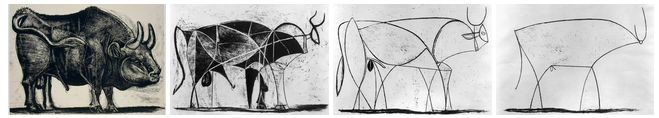
\includegraphics[width=\textwidth]{Picasso-Bull-Progression-cropped.png}
\begin{flushright}
%\emph{Bull} (plates 3, 6, 9 and 11)\\
Pablo Picasso (1881-1973)\end{flushright}
% http://www.artyfactory.com/art_appreciation/animals_in_art/pablo_picasso.htm
%\vspace{-5px}
% \begin{quote}\textit{The recent development of programming languages suggests that the simul\-taneous achievement of simplicity 
% and generality in language design is a serious unsolved 
% problem.}\begin{flushright}--- John Reynolds (1970) \cite{Reynolds70}\end{flushright}
% \end{quote}
%\begin{quote}
%\textit{Try to imagine that you are a tree. How do you want to look out here?}
%\textit{You want your tree to have some character.}
%\begin{flushright} --- Bob Ross, \emph{The Joy of Painting}\end{flushright}
%\end{quote}

% \vspace{-7px}
\section{Motivation}\label{sec:intro-motivation}
% \vspace{-6px}
%Programming languages come in many sizes. The smallest languages -- for example, the various ``lambda calculi'' -- isolate language primitives of interest for the benefit of students, researchers and language designers interested in studying their mathematical properties. These studies inform the design of ``full-scale'' programming 
%\footnote{Throughout this work, words and phrases that should be read as having an intuitive or informal meaning, rather than a strict mathematical meaning, will be introduced with quotation marks.} 
% languages, which combine several such primitives, or generalizations thereof. Full-scale languages are interesting objects of formal study in their own right. They also serve as useful tools for software developers, allowing them to construct, reason about and modularly organize large software systems.
% A single mathematical structure can often take on many syntactic forms. 
% Formal mathematical structures often come equipped with
% Experienced mathematicians and programmers define formal structures \emph{compositionally}, drawing from libraries by instantiating more abstract structures. This ultimately increases productivity, because clients of these abstract structures do not need to expend effort to establish the associated definitions and proofs anew, for each specialized structure of interest. %Instead, they need only instantiate the definitions and proofs established by a library provider in a more abstract setting.

Experienced mathematicians and programmers define formal structures \emph{compositionally}, drawing from libraries of ``general-purpose'' abstractions. The problem that motivates this work is that the resulting terms are sometimes syntactically unwieldy, and, therefore, cognitively costly. % This can neutralize the cognitive benefits of abstraction and composition. We go, therefore, in search of a mechanism of syntactic control that maintains strong compositional reasoning principles. %This can lower productivity, readability and other quality attributes of interest.  %This saves time, one does not need to establish associated definitions and proofs anew, for each specialized structure of interest.

Consider, for example, natural numbers. It is straightforward to define the natural numbers, $n$, with an inductive structure:
\[ n ::= \textbf{z} ~\vert~ \textbf{s}(n)\]
By defining natural numbers inductively, we immediately inherit a \emph{structural induction principle} -- we can establish that some property $P$ holds over the natural numbers if we establish $P(\textbf{z})$ and $P(\textbf{s}(n))$ assuming $P(n)$. The problem, of course, is that drawing particular natural numbers by repeatedly applying $\textbf{s}$ very quickly becomes syntactically unwieldy (in fact, the syntactic cost of the drawing grows linearly with $n$.)\footnote{We use the word ``drawing'' throughout this document to emphasize that syntactic cost is a property of the visual representation of a structure, rather than a semantic property.}

Similarly, it is easy to define lists of natural numbers with an inductive structure:
\[ \vec{n} ::= \textbf{nil} ~\vert~ \textbf{cons}(n, \vec{n}) \]
The problem once again is that drawings of particular lists quickly become unwieldy, and fail to resemble ``naturally occurring'' drawings of lists of numbers.

Consider a third more sophisticated example (which will be of particular relevance later in this work): when defining a programming language or logic, one often needs various sorts of tree structures equipped with metaoperations\footnote{...so named to distinguish them from the ``object level'' operations of the language being defined.} related to variable binding, e.g. substitution. Repeatedly defining these structures ``from scratch'' is quite tedious, so language designers have instead developed  a more general structure: the \emph{abstract binding tree (ABT)} \cite{Aczel78,pfpl,gabbay2002new}. Briefly, an ABT is an ordered tree structure, classified into one of several \emph{sorts}, where each node is either a \emph{variable}, $x$, or an \emph{operation} of the following form:
%\footnote{Some prior exposure to (single-sorted) ASTs is assumed here. See Sec. \ref{sec:preliminaries} for other preliminaries.} 
\begin{equation*}
\abop{op}{\vec{x}_1.\mathit{a}_1; \ldots; \vec{x}_n.\mathit{a}_n}
\end{equation*} 
where $\texttt{op}$ identifies an \emph{operator} and each of the $n \geq 0$ \emph{arguments} $\vec{x}_i.\mathit{a}_i$ binds the (possibly empty) sequence of variables $\vec{x}_i$ within the subtree $a_i$. The left side of the syntax chart in Figure \ref{fig:simple-example} summarizes the relevant operational forms for a sort called $\mathsf{CalcExp}$. ABTs of this sort are the expressions of a small arithmetic programming language,  $\simplelang$. By using  ABTs as infrastructure in the definition of $\simplelang$, we need not manually define the ``boilerplate'' metaoperations, like substitution, and reasoning principles, like structural induction, that are necessary to define $\simplelang$'s semantics and to prove it correct. {Harper gives a detailed account of ABTs, and many other examples of their use, in his book \cite{pfpl}.} 

 %and reasoning principles, e.g. {structural induction}, so we need not define this  machinery manually. 
% -- the arities of the operators can be read off from these forms ($\anumintro{n}$ is a number-indexed family of nullary operators.) 

\begin{figure}
\hspace{-5px}$\begin{array}{lrlllll}
\textbf{Sort} & & & \textbf{Operational Form} & \textbf{Stylized Form} & \textbf{Textual Form} & \textbf{Description}\\
\mathsf{CalcExp} & e & ::= & x & x & x & \text{variable}\\
&&& \aletplain{e}{x}{e} & \letplain{x}{e}{e} & \letplain{x}{e}{e} & \text{binding}\\
&&& \anumintro{n} & \numintro{n} & \numintro{n} & \text{numbers}\\
&&& \aplus{e}{e} & e + e & e\texttt{ + }e & \text{addition} \\
% &&& \aminus{e}{e} & e - e & e\texttt{ - }e & \text{subtraction}\\
&&& \amult{e}{e} & e \times e & e\texttt{ * }e & \text{multiplication}\\
&&& \adiv{e}{e} & \frac{e}{e} & e\texttt{ / }e & \text{division}\\
&&& \apow{e}{e} & {e}^{e} & e\verb|^|e & \text{exponentiation}\\
\end{array}$
\caption[Syntax of $\simplelang$]{Syntax of $\simplelang$. Metavariable $n$ ranges over natural numbers and $\numintro{n}$ abbreviates the numeral forms (one for each natural number $n$, drawn in \texttt{typewriter} font.) A formal definition of the stylized and textual syntax of $\simplelang$ would require 1) defining these numeral forms explicitly; 2) defining a parenthetical form; 3) defining the precedence and associativity of each infix operator; and 4) defining whitespace conventions.}
\label{fig:simple-example}
% \vspace{-5px}
\end{figure}

% \subsection{Syntax Matters}
The problem with this approach is, again, that drawing a non-trivial $\simplelang$ expression in operational form is syntactically costly. For example, we will consider the following drawing in our discussion below:
\begin{subequations}\label{drawings:simple}\begin{equation}\label{simple-example-op-form}
\adiv{\anumintro{\textbf{s}(\textbf{z})}}{
	\apow{\anumintro{\textbf{s}(\textbf{s}(\textbf{z}))}}{\adiv{\anumintro{\textbf{s}(\textbf{z})}}{\anumintro{\textbf{s}(\textbf{s}(\textbf{z}))}}}
}\end{equation}
% This is an example of a common problem: instantiating a general-purpose abstraction, here for defining ABTs, can be  structurally economical but  \emph{syntactically costly} (or \emph{cognitively costly} in some other sense, as we will discuss in Section \ref{sec:syntactic-properties}.) Mathematics is ultimately a human activity, so these costs are worthy of consideration.

\subsection{Informal Mathematical Practice}
Within a document intended only for human consumption, it is easy to informally outline less costly alternative syntactic forms. 

For example, mathematicians generally use the Western Arabic numeral forms when drawing particular natural numbers, e.g. $2$ is taken as a syntactic alternative to $\textbf{s}(\textbf{s}(\textbf{z}))$. 

Similarly, mathematicians might informally define alternative list forms, e.g. $[0, 1, 2]$ as a syntactic alternative to: 
\[\textbf{cons}(\textbf{z}, \textbf{cons}(\textbf{s}(\textbf{z}), \textbf{cons}(\textbf{s}(\textbf{s}(\textbf{z})), \textbf{nil})))\]

The middle columns of the syntax chart in Figure \ref{fig:simple-example} suggest two alternative forms for every ABT of sort $\mathsf{CalcExp}$. We can draw the ABT from Drawing (\ref{simple-example-op-form}) in an alternative \emph{stylized form}:
% div(num[1]; pow(num[2]; div(num[1]; num[2]))
% \begin{subequations}
% \begin{equation}\label{simple-example-op-form}
% \adiv{\anumintro{1}}{
% 	\apow{\anumintro{2}}{\anumintro{3}}
% }\end{equation}
\begin{equation}\label{simple-example-sty-form}
\frac{\numintro{1}}{{\numintro{2}^{\frac{\numintro{1}}{\numintro{2}}}}}
\end{equation}
or in an alternative \emph{textual form}:
\begin{equation}\label{simple-example-txt-form}
\texttt{1 / 2\textasciicircum(1/2)}
\end{equation}
\end{subequations}

Mathematicians also sometimes supplement alternative primitive forms like these with various \emph{derived forms}, which  identify ABTs indirectly according to stated context-independent \emph{desugaring rules}. For example, the following desugaring rule defines a derived stylized form for square root calculations:
% \begin{subequations}
% \begin{subequations}[intermezzo]
\begin{equation}\label{rule:simplelang-sqrt}
\sqrt{e} \rightarrowtriangle e^{\frac{\numintro{1}}{\numintro{2}}}
\end{equation}
% \end{subequations}
The reader can desugar a drawing of an ABT by recursively applying desugaring rules wherever a syntactic match occurs. A desugared drawing consists only of the {primitive forms} from Figure \ref{fig:simple-example}. 
For example, the following drawing desugars to Drawing (\ref{simple-example-sty-form}), which in turn corresponds to Drawing (\ref{simple-example-op-form}) as discussed above:
\begin{equation*}\tag{\ref*{drawings:simple}d}
\frac{\numintro{1}}{\sqrt{\numintro{2}}}
\end{equation*}
%No new operators are introduced.

% Syntactically, however, this practice has its limits. 

% Mathematicians often invent specialized syntactic forms in order to visually represent the formal structures that they define. 
% % For example, Figure \ref{fig:simple-example} defines three different ways to draw any abstract syntax tree (AST) of sort  $\mathsf{CalcExp}$. ASTs of this sort are the expressions of a small arithmetic programming language, $\simplelang$.\footnote{Some familiarity with abstract syntax trees is preliminary to this work. See Sec. \ref{sec:preliminaries} for citations and a more thorough discussion of preliminaries.}
% % Mathematicians, like painters, exercise creative license when they draw the structures that arise in their work. 
% % Mathematicians, like painters, exercise creativity when they draw the structures that arise in their work. 
% % Mathematicians often define structurally redundant syntactic forms. 
% %, i.e. forms that are syntactically distinct but that identify the same formal structure. 
% % When defining the syntax of a programming language, language designers often define structurally redundant syntactic forms. 
% % Mathematicians, like painters, draws these trees in a variety of styles.  
% % There are many ways to draw trees of this sort. 
% % There are many ways to draw a tree. 
% % Most formal structures are defined as modes of use of more primitive formal structures. For example, the expressions of a variety of programming languages are all defined as particular sorts of \emph{abstract syntax trees}.  
% For example, the three drawings below all identify the same tree structure  of sort $\mathsf{CalcExp}$, differing according to the syntax chart in Figure \ref{fig:simple-example} only in that the first drawing is in a general \emph{operational form}, whereas the second drawing is in a specialized \emph{stylized form} and the third is in a specialized \emph{textual form}:
% %
% % differing only in that Drawing (\ref*{simple-example-op-form}) is in \emph{operational form}, Drawing (\ref*{simple-example-sty-form}) is in \emph{stylized form} and Drawing (\ref*{simple-example-txt-form}) is in \emph{textual form}:
% \begin{subequations}
% \begin{equation}\label{simple-example-op-form}
% \adiv{\anumintro{1}}{
% 	\apow{\anumintro{2}}{\anumintro{3}}
% }\end{equation}
% \begin{equation}\label{simple-example-sty-form}
% \frac{\numintro{1}}{{\numintro{2}^{\numintro{3}}}}
% \end{equation}
% \begin{equation}\label{simple-example-txt-form}
% \texttt{1 / 2\textasciicircum3}
% \end{equation}
% \end{subequations}
% \noindent
% Trees of this sort are the expressions of $\simplelang$, a simple arithmetic programming language. 

% These drawings identify the same AST, meaning that they are all drawn from the same row of the syntax chart at every level. In other words, these drawings are structurally indistinct. 

% In particular, let us consider a simple programming language, $\simplelang$, for performing arithmetic calculations with numbers. The expressions of $\simplelang$ are \emph{abstract syntax trees (ASTs)} of a sort defined by the syntax chart in Figure \ref{fig:simple-example}.\footnote{Familiarity with abstract syntax trees is preliminary to this work (see Sec. \ref{sec:preliminaries} for other preliminaries.)}  For example, the following expression is drawn in stylized form:
% The same expression is drawn in textual form as follows:
% \noindent
% and in operational form as follows:

When defining the semantics of a language like $\simplelang$, it is customary to adopt an \emph{identification convention} whereby drawings that identify the same underlying ABT structure, like Drawings (\ref{drawings:simple}), are considered interchangeable. %only if they are drawn from different rows of the syntax chart in Figure \ref{fig:simple-example}. 
For example, consider the semantic  judgement $\isvalU{e}$, which establishes certain  $\simplelang$ expressions as \emph{values} (as distinct from expressions that can be arithmetically simplified or that are erroneous.) The following inference rule establishes that every number expression is a value:\footnote{Some familiarity with inductively defined judgements and inference rules like these is preliminary to this work. See Sec. \ref{sec:preliminaries} for citations and further discussion of necessary preliminaries.}
\begin{equation}\label{rule:num-val}
\inferrule{ }{
	\isvalU{\anumintro{n}}
}
\end{equation}
Although this rule is drawn using the operational form for number expressions, we can apply it to derive that $\isvalU{\numintro{2}}$, because $\numintro{2}$ and $\anumintro{2}$  identify the same ABT.

% In summary, it is both the case that ``syntax doesn't matter'' (semantically) and that syntax matters (cognitively). %i.e.  because mathematics is a human activity that alternative and derived forms matter (cognitively).%Syntax matters because mathematics and programming are human activities. 


% \subsection{Syntax Doesn't Matter  (Semantically)}
% It is worth emphasizing here that these common syntactic practices are not motivated by semantic considerations. Indeed, 



% \subsection{Syntax Matters (Cognitively)}
% %Our semantics would be no weaker if we had defined only, for example, the operational forms. 
% %The answer, of course, is that from the perspective of a human programmer, syntax \emph{does} matter. 
% % If different drawings of a $\simplelang$ expression are not semantically distinguishable, why did we bother to define alternative syntactic forms at all?
% Syntactic sugar matters because mathematics and programming are human activities. Different visual representations of a formal structure can and must be distinguished by the \emph{cognitive costs} that human programmers incur as they produce or examine them.\footnote{In fact, we should be interested in sensory modalities other than vision, if only because many humans lack sufficient eyesight. Alas, this topic is beyond the scope of our present work.}% Drawings of formal structures serve as \emph{user interfaces} to the underlying structures themselves.

% For example, a human programmer might distinguish drawings of $\simplelang$ expressions in stylized or textual form, like Drawings (\ref{simple-example-sty-form}) through (\ref{simple-example-derived-form}) above, as less ``crowded'' and more ``familiar'' than those in operational form, because they follow the usual arithmetic conventions or close approximations thereof. This might help the human  programmer extract meaning from such drawings more quickly. Similarly, drawings in textual form involve only text, which can lower the costs involved in their production. Of course, drawings in operational form can bring cognitive benefits as well -- dispensing with various syntactic complexities (e.g. related to  precedence and associativity) can simplify metatheoretic reasoning and implementation efforts. 

% We will cover more rigorous operationalizations of the necessarily broad notion of cognitive cost in Section \ref{sec:syntactic-properties}. %Mistakes may also be less frequent when producing drawings in stylized or textual form (for $\simplelang$ expressions, perhaps only because operational forms use more parentheses). 

% \subsection{Derived Forms}
% %The forms defined by the syntax chart in Figure \ref{fig:simple-example} suffice to allow programmers to draw any $\simplelang$ expression. However, 
% In seeking to lower cognitive costs, syntax designers  often  include additional \emph{derived forms}  in a syntax definition. Unlike the \emph{primitive forms}  defined in Figure \ref{fig:simple-example}, which identify trees directly, derived forms identify trees indirectly, through a context-independent {desugaring} rule.   
% %We can define a desugaring transformation by stating a rewrite rule. 
% For example, the following desugaring rule defines a derived stylized form for calculating the square root of a $\simplelang$ expression:
% % \begin{subequations}
% \begin{equation}\label{rule:simplelang-sqrt}
% \sqrt{e} \rightarrowtriangle e^{\frac{\numintro{1}}{\numintro{2}}}
% \end{equation}
% % Similarly, the following rewrite rule, if included in the definition of the textual syntax of expressions, defines a derived form for negating a $\simplelang$ expression:\footnote{Notice that the right-hand side of this rule is in operational form, rather than textual. For $\footnotesimplelang$, it is not necessary to prevent textual and operational forms from being interspersed within a single drawing -- no ambiguities can arise. For richer syntax definitions, this may no longer be the case. The desugaring process must then be modified to first convert the pattern on the righthand side of a desugaring rule like Rule (\ref{rule:simplelang-negate}) to the desired form variant before it is applied.}
% % \begin{equation}\label{rule:simplelang-negate}
% % \texttt{-}e \rightarrowtriangle \amult{e}{\anumintro{-1}}
% % \end{equation}
% % \end{subequations}
% % \noindent 
% Desugaring a drawing of a tree involves first recursively desugaring the drawings of its subtrees. If the drawing is in primitive form, desugaring is complete.  If the drawing is in derived form, we apply the corresponding desugaring rule (here, we  have only one choice.) The desugared drawing will identify a tree immediately, i.e. it will consist only of primitive forms. No new trees are introduced, so the semantics is unchanged. %Derived forms affect only cognitive cost.
%Similarly, we might define a derived form for taking an arbitrary root of an expression as follows:
% \begin{align*}
% \sqrt[e']{e} & \rightarrowtriangle e^{\frac{\numintro{1}}{e'}}
% \end{align*}

\subsection{Derived Forms in General-Purpose Languages}
We would need to define only a few more derived arithmetic forms to satisfyingly capture the  idioms that arise in the limited domains where a simple language of arithmetic operations like $\simplelang$ might be useful. %Consequently, there is little opportunity to go beyond simple derived forms like these. 
However, programming languages in common use today are substantially more semantically expressive. Indeed, many mathematical structures, including natural numbers, lists and ABTs, can be adequately expressed within contemporary ``general-purpose'' programming languages. %Mathematics has become supplanted by particular formal system. 
Consequently, the problems of syntactic cost just discussed at the level of the ambient mathematics also arise ``one level down'', i.e. when writing programs. For example, we want syntactic sugar not only for mathematical natural numbers, lists and $\simplelang$ expressions, but also for \emph{encodings} of these structures within a general-purpose programming language.% .) %https://github.com/jonsterling/sml-abt or https://github.com/RedPRL/sml-typed-abts.) 

We can continue to rely on the informal notational conventions described above only as long as programs are drawn solely for human consumption. These conventions break down when we need drawings of programs to themselves exist as formal structures suitable for consumption by other programs, i.e. \emph{parsers}, which check whether drawings are well-formed relative to a \emph{syntax definition} and produce structures suitable for consumption by yet other programs, e.g. compilers. %This, of course, is the regime of contemporary computer programming.

% The problem is that nearly all contemporary languages are designed so that drawings of programs can be consumption both by humans and by another program -- a parser -- which checks whether drawings are well-formed and produces a structure suitable for consumption by various other useful programs, e.g. editors and compilers.


% Programmers address these problems by informally stating alternative and derived forms, as in handwritten or typeset mathematics, because a drawing of a program must be suitable for consumption both by humans and by % This limits the control that programmers have over syntactic cost.

% In contemporary practice, other programs -- parsers -- consume drawings of programs, which generate corresponding structures for execution by modern computer hardware. As such, we cannot rely on an informal approach that defers ultimately to the intuitions of a human reader. Instead, we must define the syntactic conventions that we wish to use with rigor. 

Constructing a formal syntax definition is not itself an unusually difficult task for an experienced programmer, and there are many \emph{syntax definition systems} that help with this task (Sec. \ref{sec:existing-approaches} will cover several examples.) The problem is that when designing the syntax of a general-purpose language, the language designer cannot hope to anticipate all library constructs for which derived forms might one day be useful. At best, the language designer can bundle certain libraries together into a ``standard library'', and privilege select constructs defined in this library with derived forms. 

% as these ``general-purpose'' languages have evolved, many other derived forms have become incorporated into their syntax definitions.\footnote{The same dynamic is apparent in the progression of ``pen and paper'' and typeset mathematics.}  
For example, the textual syntax of Standard ML (SML), a general-purpose language in the functional tradition, defines derived forms for constructing and pattern matching on lists \cite{mthm97-for-dart,harper1997programming}. In SML, the derived expression form \lstinline{[x, y, z]} desugars to an expression equivalent to:
\begin{lstlisting}[numbers=none]
Cons(x, Cons(y, Cons(z, Nil)))
\end{lstlisting}
assuming \li{Nil} and \li{Cons} stand for the list constructors exported by the SML Basis library (i.e. SML's ``standard library''.)\footnote{The desugaring actually uses unforgeable identifiers bound permanently to the list constructors, to ensure that the desugaring is context independent. We will return to the concept of context independence throughout this work.} Other languages similarly privilege select standard library constructs with derived forms:

\begin{itemize}
\item OCaml \cite{ocaml-manual} defines derived forms for strings (defined as arrays of characters.)
\item Haskell \cite{jones2003haskell} defines derived forms for encapsulated commands (and, more generally, values of any type equipped with monadic structure.)
\item Scala \cite{odersky2008programming} defines derived XML forms as well as string splicing forms, which capture the idioms of string concatenation.
\item F\# \cite{syme2012expert}, Scala \cite{shabalin2013quasiquotes} and various other languages define derived forms for encodings of the language's own terms (these are referred to as \emph{quasiquotation} forms.)
\item Python \cite{python} defines derived forms for mutable sets and dictionaries.
\item Perl \cite{perlre} defines derived regular expression forms.
\end{itemize}

These choices are, fundamentally, made according to \emph{ad hoc} design criteria -- there are no clear semantic criteria that fundamentally distinguish standard library constructs privileged with derived forms from those defined in third-party libraries. 
%Indeed, it is considered a virtue for a standard library can be separated from the language definition. 
Indeed, as the OCaml community has moved away from a single standard library in favor of competing bundles of third-party libraries (e.g. Batteries Included \cite{OCaml-batteries} and Core \cite{OCaml-core}), this approach has become starkly impractical.% This puts into question the practice of bundling a single standard library with  entirely.

\section{Existing Mechanisms of Syntactic Control}
A more parsimonious approach would be to eliminate derived forms  specific to standard library constructs from language definitions in favor of mechanisms that give more syntactic control to third-party library providers.

In this section, we will give a brief overview of existing such mechanisms and speak generally about the problems that they present to motivate our novel contributions in this area. We will return to give a detailed overview of these various existing mechanisms of syntactic control in Section \ref{sec:existing-approaches}. 

\subsection{Syntax Dialects}\label{sec:problems-with-dialects}
One approach that a library provider can take when seeking more syntactic control is to use a syntax definition system to construct a \emph{syntax dialect}, i.e. a new syntax definition that extends the original syntax definition with new derived forms. 
%library-specific (a.k.a. ``domain-specific'') 

For example, Ur/Web extends Ur's textual syntax with derived forms for SQL queries, XHTML elements and other constructs defined in a  web programming library \cite{conf/popl/Chlipala15,conf/pldi/Chlipala10}. Figure \ref{fig:urweb} demonstrates how XHTML expressions that contain strings can be drawn in Ur/Web. The desugaring of this derived form (not shown) is substantially more verbose and, for programmers familiar with the standardized syntax for XHTML \cite{xhtml}, substantially more obscure. % Such dialects are sometimes qualitatively taxonomized as amongst the ``domain-specific language'' for this reason \cite{fowler2010domain}. %Syntactic cost is often assessed qualitatively \cite{green1996usability}, though quantitative metrics can be defined. 
\begin{figure}[h]
\begin{lstlisting}[numbers=none]
val p = SURL<xml><p>Hello, {[EURLjoin " " [first, last]SURL]}!</p></xml>EURL
\end{lstlisting}
\caption{Derived XHTML forms in Ur/Web}
\label{fig:urweb}
\end{figure}                           

Syntax definition systems like Camlp4 \cite{ocaml-manual}, Copper \cite{conf/gpce/WykS07} and SugarJ/Sugar* \cite{erdweg2011sugarj,erdweg2013framework}, which we will discuss in Sec. \ref{sec:syntax-dialects}, have simplified the task of defining ``library-specific'' (a.k.a. ``domain-specific'') syntax dialects like Ur/Web, and have thereby contributed to their ongoing proliferation.
%The desugaring, not shown, is substantially more verbose and, for programmers who are familiar with XHTML forms, substantially more obscure than the drawing above. %We will consider other examples of data structures where syntactic cost becomes a legitimate concern for client programmers in Sec. \ref{sec:motivating-examples}. 
%after first reviewing simpler approaches that also help library providers control syntactic cost, albeit to a more limited extent, 
% Syntax definition systems 
% The most syntactically expressive of the mechanisms that we will detail in Section \ref{sec:existing-approaches} are 


%Full-scale languages are also interesting objects of mathematical study. Uniquely, however, they are also designed for use by humans. Consequently, their designers  typically define both an abstract syntax and a textual syntax. This textual syntax serves as the primary interface between human programmers and the language, so it is common to define various \emph{derived forms}, i.e. forms defined by a context-independent \emph{desugaring} to a set of \emph{base forms}. These serve to decrease the \emph{syntactic cost} or \emph{cognitive cost} of selected idioms. 
%In some cases, a derived form is designed to capture an idiom77Gu that involves only the primitive constructs of the language. 

%The hope amongst some language designers is that a limited number of derived forms like these will suffice to produce a ``general-purpose'' textual syntax, i.e. one that is accepted as suitable for use across a wide variety of application domains. Alas, a stable design that fully achieves this ideal has yet to emerge, as evidenced by the diverse array of \emph{syntax dialects} -- dialects that introduce only new derived forms -- that continue to proliferate around all major contemporary languages. 

%In fact, tools that aid in the construction of so-called  ``domain-specific'' language dialects (DSLs)\footnote{In some parts of the literature, such dialects are called ``external DSLs'', to distinguish them from  ``internal'' or ``embedded DSLs'', which are actually  library interfaces that only ``resemble'' distinct dialects \cite{fowler2010domain}.} seem only to be becoming more prominent over time. 

%\subsection{Why are there so many language dialects?}
%{This calls for an investigation}: why is it that programmers and researchers are still so often unable to satisfyingly express the constructs that they seek in libraries, as modes of use of the ``general-purpose'' primitives already available in major languages today, and instead see a need for new language dialects?

%Perhaps the most common sort of dialect is the \emph{syntax dialect} -- a dialect that introduces only new derived syntactic forms, motivated by a desire to decrease the {syntactic cost} of working with one or more library constructs of interest. 
%Put another way, syntax dialects can be specified by a context-independent expansion to the existing language that they are based on. 
%For example, Ur/Web is a syntax dialect of Ur (a language that itself descends from ML \cite{conf/pldi/Chlipala10}) that builds in derived forms for SQL queries, HTML elements and other datatypes used in the domain of web programming \cite{conf/popl/Chlipala15}. %Syntactic cost is often assessed qualitatively \cite{green1996usability}, though quantitative metrics can be defined. 
%This is not an isolated example -- we will consider a number of additional types of data that similarly stand to benefit from the availability of specialized derived forms in Sec. \ref{sec:motivating-examples}. 
%Tools like Camlp4 \cite{ocaml-manual}, Sugar* \cite{erdweg2011sugarj,erdweg2013framework} and Racket \cite{Flatt:2012:CLR:2063176.2063195}, which we will discuss in Sec. \ref{sec:existing-approaches}, have lowered the engineering costs of constructing syntax dialects in such situations, further contributing to their proliferation. 

%More advanced dialects introduce new type structure, going beyond what is possible with only new derived forms. As a simple example, the static and dynamic semantics of records cannot be expressed by context-independent expansion to a language with only nullary and binary products. Various languages have explored ``record-like'' primitives that go further, supporting functional update operators, width and depth coercions (sometimes implicit)%\cite{Cardelli:1984:SMI:1096.1098}
%, methods, prototypic dispatch and other such ``semantic embellishments'' that in turn cannot be expressed by context-independent expansion to a language with only standard record types (we will detail an  example in Sec. \ref{sec:metamodules-motivating-examples}). OCaml primitively builds in the type structure of polymorphic variants, open datatypes and  operations that use format strings like $\mathtt{sprintf}$ \cite{ocaml-manual}. ReactiveML builds in primitives for functional reactive programming \cite{mandel2005reactiveml}. ML5 builds in high-level primitives for distributed programming based on a modal lambda calculus \cite{Murphy:2007:TDP:1793574.1793585}. Manticore \cite{conf/popl/FluetRRSX07} and AliceML  \cite{AliceLookingGlass} build in parallel programming primitives with a more elaborate type structure than is found in simpler accounts of parallelism. 
%MLj builds in the type structure of the Java object system (motivated by a desire to interface safely and naturally with Java libraries) \cite{Benton:1999:IWW:317636.317791}. Other dialects do the same for other foreign languages, e.g. Furr and Foster describe a dialect of OCaml that builds in the type structure of C \cite{Furr:2005:CTS:1065010.1065019}. Tools like proof assistants and logical frameworks are used to specify and reason metatheoretically about dialects like these, and tools like compiler generators and language frameworks \cite{erdweg2013state} lower their implementation cost, again contributing to their proliferation. 

% \vspace{-5px}
%\subsection{Problems with the Dialect-Oriented Approach}\label{sec:problems-with-dialects}
Many have argued that a proliferation of syntax dialects is harmless or even desirable, because programmers can simply choose the right syntax dialect for each job at hand \cite{journals/stp/Ward94}. However, we argue that this ``dialect-oriented approach'' is difficult to reconcile with the best practices of ``programming in the large''  \cite{DeRemer76}, i.e. developing large programs ``consisting of many small programs (modules), possibly written by different people'' whose interactions are mediated by a reasonable type and binding discipline. The problems that tend to arise are summarized below; a more systematic treatment will follow in  Sec. \ref{sec:syntax-dialects}.

\subsubsection{Problem 1: Conservatively Combining Syntax Dialects}
The first problem with the dialect-oriented approach is that clients  cannot always combine different syntax dialects when they want to use derived forms that they define together. This is problematic because client programs  cannot be expected to fall cleanly into a single preconceived ``problem domain'' -- large programs use many libraries \cite{DBLP:conf/sac/LammelPS11}.

For example, consider a syntax dialect, $\mathcal{H}$, defining derived forms for working with encodings of HTML elements, and another syntax dialect, $\mathcal{R}$,  defining derived forms for working with encodings of regular expressions. Some programs will undoubtedly need to manipulate HTML elements as well as regular expressions, so it would be useful to construct a ``combined dialect'' where all of these derived forms are defined. 

For this notion of ``dialect combination'' to be well-defined at all, we must first have that $\mathcal{H}$ and $\mathcal{R}$ are defined under the same syntax definition system. In practice, there are many useful syntax definition systems, each differing subtly from the others. %If the dialect designers  have not  chosen the same syntax definition system, then ``dialect combination'' is not systematic (in the way that importing different libraries is systematic.)%$\mathcal{H} \cup \mathcal{R}$ is simply undefined.% (e.g. parser combinator libraries like Haskell's \li{parsec} \cite{parsec}.)

If $\mathcal{H}$ and $\mathcal{R}$ are coincidentally defined under the same syntax definition system, we must also have that this system operationalizes the notion of dialect combination, i.e. it must define some operation $\mathcal{H} \cup \mathcal{R}$ that creates a dialect that extends both $\mathcal{H}$ and $\mathcal{R}$, meaning that any form defined by either $\mathcal{H}$ or $\mathcal{R}$ must be defined by $\mathcal{H} \cup \mathcal{R}$. Under systems that do not define such an operation (e.g. Racket's dialect preprocessor \cite{Flatt:2012:CLR:2063176.2063195}), clients can only manually  ``copy-and-paste'' or factor out portions of the constituent dialect definitions to construct the ``combined'' dialect. This is not systematic and, in practice, it can be quite tedious and error-prone. %In both this and the previous case, ``dialect combination'' is a strictly informal notion, left to library clients to operationalize through manual labor (hence the quotes).

Even if we restrict our interest  to dialects defined under a common syntax definition system that does operationalize the notion of dialect combination (or similarly one that allows clients to systematically combine \emph{dialect fragments}), we still have a problem: there is generally no guarantee that the combined dialect will conserve important properties that can be established about the constituent dialects in isolation (i.e. \emph{modularly}.) In other words, establishing $P(\mathcal{H})$ and $P(\mathcal{R})$ is not sufficient to establish $P(\mathcal{H} \cup \mathcal{R})$ for many useful properties $P$. Clients must re-establish such properties for each combined dialect that they construct.%In other words, any putative ``combined language'' must formally be considered a  distinct system for which one must derive essentially all metatheorems of interest anew, guided only informally by those derived for the dialects individually. %There is no well-defined mechanism for constructing such a ``combined language'' in general. 

One important property of interest is \emph{syntactic determinism} -- that every derived form has at most one desugaring. It is not difficult to come up with examples where combining two deterministic syntax dialects produces a non-deterministic dialect. For example, consider two syntax dialects defined under a system like Camlp4: $\mathcal{D}_1$ defines derived forms for sets, and $\mathcal{D}_2$ defines derived forms for finite maps, both delimited by \verb~{<~ and \verb~>}~.\footnote{In OCaml, simple curly braces are already reserved by the language for record types and values.} Though each dialect defines a deterministic grammar, i.e. $\mathrm{det}(\mathcal{D}_1)$ and $\mathrm{det}(\mathcal{D}_2)$, when the grammars are na\"ively combined by Camlp4, we do not have that $\mathrm{det}(\mathcal{D}_1 \cup \mathcal{D}_2)$ (i.e. syntactic ambiguities arise under the combined dialect.) In particular, \verb~{<>}~ can be recognized as either the empty set or the empty finite map. %A recent version of Python added derived forms for mutable sets. Due to a conflict with dictionary syntax, however, there is no derived form for the empty set.)
 %A third syntax dialect might come along that uses the same forms that $\mathcal{D}_2$ defines, but for ordered finite maps.

Schwerdfeger and Van Wyk have developed a modular grammar-based syntax definition system, implemented in Copper \cite{conf/gpce/WykS07}, that guarantees that determinism is conserved when syntax dialects (of a certain restricted class) are combined \cite{conf/pldi/SchwerdfegerW09,schwerdfeger2010context} as long as each constituent dialect prefixes all newly introduced forms with starting tokens drawn from disjoint sets. We will describe the difficulties that this requirement causes in Section \ref{sec:syntax-dialects}.


\subsubsection{Problem 2: Abstract Reasoning About Derived Forms}\label{sec:abs-reasoning-intro}
Even putting aside the difficulties of conservatively combining syntax dialects, there are questions about how \emph{reasonable}  sprinkling library-specific derived forms throughout a large software system might be. 
For example, consider the perspective of a programmer attempting to comprehend (i.e. reason about) the program fragment in Figure \ref{fig:K-dialect}, which is drawn under a syntax dialect constructed by combining a number of dialects of Standard ML's textual syntax.

\begin{figure}[h]
\begin{lstlisting}
val w = compute_w ()
val x = compute_x w
val y = {|(!R)@&{&/x!/:2_!x}'!R}|}
\end{lstlisting}
\caption{An example of unreasonable program text}
\label{fig:K-dialect}
\end{figure}

If the programmer happens to be familiar with the (intentionally terse) syntax of the stack-based database query processing language K \cite{Whitney:2001:LOR:376284.375783}, then Line 3 might pose few difficulties. If the programmer does not recognize this syntax, however, there are no simple, definitive protocols for answering questions like:
\begin{enumerate}
\item \textbf{(Responsibility)} Which constituent dialect defined the derived form that appears on Line 3?
\item \textbf{(Segmentation)} Are the characters \li{x} and \li{R} on Line 3 parsed as spliced expressions \li{x} and \li{R} (i.e. expressions of variable form), or parsed in some other way peculiar to this form?
\item \textbf{(Capture)} If \li{x} is in fact a spliced expression, does it refer to the binding of \li{x} on Line 2? Or might it capture an unseen binding introduced in the desugaring of Line 3?
\item \textbf{(Context Dependence)} If \li{w}, on Line 1, is renamed, could that possibly break the program, or change its meaning? In other words, might the desugaring of Line 3 assume that some variable identified as \li{w} is in scope (even though \li{w} is not mentioned in the text of Line 3)?
\item \textbf{(Typing)} What type does \li{y} have?
\end{enumerate}

In short, syntax dialects do not come with useful principles of \emph{syntactic abstraction}: if the desugaring of the program is held abstract, programmers can no longer reason about types and binding (i.e. answer questions like those above) in the usual disciplined manner. This is burdensome at all scales, but particularly when programming in the large, where it is common to encounter a program fragment drawn by another programmer, or drawn  long ago. Forcing the programmer to examine the desugaring of the drawing in order to reason about types and binding defeats the ultimate purpose of using syntactic sugar -- lowering cognitive cost (we expand on the notion of cognitive cost in Sec. \ref{sec:syntactic-properties}.) 


%In other words, encountering an unfamiliar derived form has made it difficult for the programmer to maintain the usual \emph{type discipline} and \emph{binding discipline}. %Compelling the programmer to examine the desugaring directly defeat the purpose of defining the derived form -- decreasing cognitive cost. Indeed, it substantially increases cognitive cost.

In contrast, when a programmer encounters, for example, a function call like the call to \li{compute_x} on Line 3, the analagous questions can be answered by following clear protocols that become ``cognitive reflexes'' after sufficient experience with the language, even if the programmer has no experience with the library defining \li{compute_x}:
\begin{enumerate}
\item The language's syntax definition determines that \li{compute_x w} is an expression of function application form.
\item Similarly, \li{compute_x} and \li{w} are definitively expressions of variable form.
\item The variable \li{w} can only refer to the binding of \li{w} on Line 1.
\item The variable \li{w} can be renamed without knowing anything about the value that \li{compute_x} stands for.
\item The type of \li{x} can be determined to be \li{B} by determining that the type of \li{compute_x} is \li{A -> B} for some \li{A} and \li{B}, and checking that \li{w} has type \li{A}. Nothing else needs to be known about the value that \li{compute_x} stands for. In Reynolds' words \cite{B304}:
\begin{quote}
\emph{Type structure is a syntactic discipline for enforcing levels of abstraction.}
\end{quote}
\end{enumerate}



% In summary, syntax dialects give library providers so much syntactic control that it creates problems for client programmers.
%A related issue arises when one works within a language with a module system, i.e. a system that supports interacting through a defined interface with various implementations of that interface. For example, consider different regular expression engines that differ only with regard to their performance in various circumstances, or different parser generators that accept the same class of grammar. Ideally, one would like to be able to define derived forms once such that they operate only through the common interface. To do so today requires both an awkward syntactic trick and coordination between library providers, as we will discuss in Sec. \ref{sec:syntax-examples-regexps}. Ideally, this would not be necessary.

%It is thus infeasible to simply allow different contributors to a software system to choose their own favorite dialect for each component they are responsible for. 
%It it clear that dialects are better rhetorical devices than practical engineering artifacts. 

%Due to this paucity of modular reasoning principles, the ``dialect-oriented'' approach is problematic for software development ``in the large''. %Large software projects and software ecosystems must pick a single language that does provide powerful modular reasoning principles and, to benefit from them, stay inside it.

% \subsection{Central Planning Considered Harmful}
% Dialects do sometimes have a less direct influence on large-scale software development: they can help convince the designers in control of comparatively popular languages, like OCaml and Scala, to include some variant of the primitives that they feature into backwards-compatible language revisions. %These decisions are increasingly influenced by community processes, e.g. the Scala Improvement Process.  %This approach concentrates power as well as responsibility over maintaining metatheoretic guarantees in the hands of a small group of language designers, though increasingly influenced by various community processes (e.g. the Scala Improvement Process). 
% %Dialects thus serve the role of rhetorical vehicles for new ideas, rather than direct artifacts. 
% %Over time, accepting such extensions has caused these languages to balloon in size. 
% This \emph{ad hoc} approach is unsustainable, for three main reasons. First, as we will demonstrate in Sec. \ref{sec:motivating-examples}, there are simply too  many potentially useful such primitives, and many of these capture idioms common only in relatively narrow application domains. It is unreasonable to expect language designers to be able to evaluate all of these use cases in a timely and informed manner. Second, primitives introduced earlier in a language's lifespan can end up monopolizing finite ``syntactic resources'', forcing subsequent primitives to use ever more esoteric forms. And third, primitives that prove after some time to be flawed in some way cannot be removed or modified without breaking backwards compatibility. For these reasons, language designers are justifiably reticent to add new primitives to major languages.%Because there is often no empirical data about how useful a construct is in practice until it is available in a major language, decisions about which constructs to include are often informed only by intuition (and are thus)
% %Recalling the words of  Reynolds, which are clearly as relevant today as they were almost half a century ago \cite{Reynolds70}: %This approach is antithetical to the ideal of a truly \emph{general-purpose language} described at the beginning of this section.
% %\newpage

%\subsection{Toward More Reasonable Primitives}
%These 
%This leaves two possible paths forward. One is to simply eschew ``niche'' derived forms and settle on the existing designs, which might be considered to sit at a ``sweet spot'' in the overall language design space (accepting that in some circumstances, this leads to  high cognitive cost). 


%Similarly, it recently introduced ``open datatypes'', which subsume its previous more specialized exception type, and captures many use cases for .

%Viewed ``dually'', one might equivalently ask for a language that builds in a core that is as small as possible, but provides expressive power comparable to languages with much larger cores. This is our goal in the work being proposed

%Similarly, it recently introduced ``open datatypes'', which subsume its previous more specialized exception type, and captures many use cases for .

%Viewed ``dually'', one might equivalently ask for a language that builds in a core that is as small as possible, but provides expressive power comparable to languages with much larger cores. This is our goal in the work being proposed. 

\subsection{Term Rewriting Systems}
An alternative approach that a library provider can consider when seeking to control syntactic cost is to leave the context-free syntax of the language fixed and instead contextually repurpose existing syntactic forms using a \emph{term rewriting system}. We will review various term rewriting systems in detail in Sec. \ref{sec:non-local-term-rewriting} and Sec. \ref{sec:macro-systems}. 

Na\"ive term rewriting systems suffer from problems analagous to those that plague syntax definition systems. In particular, it is difficult to conserve determinism, i.e. separately defined rewriting rules might attempt to rewrite the same term differently. Moreover, it can be difficult to determine which rewriting rule, if any, is responsible for a particular term, and to reason about types and binding given a drawing of a program subject to a large number of rewriting rules without examining the rewritten program.

Modern \emph{term-rewriting macro systems}, however, have made some progress toward addressing these problems. In particular:
\begin{enumerate}
\item Macro systems require that the client explicitly apply the intended rewriting (implemented by a macro) to the term that is to be rewritten, thereby addressing the problems of conflict and determining responsibility. However, it is often unclear whether a given macro  is repurposing the form of a given argument or sub-term thereof, as opposed to treating it parametrically by inserting it unmodified into the generated expansion. This is closely related to the problem of determining a {segmentation}, discussed above.
\item Macro systems that enforce \emph{hygiene}, which we will return to in Sec. \ref{sec:macro-systems}, address many of the problems related to reasoning about binding. 
\item The problem of reasoning about types has been relatively understudied, because most research on macro systems has been for languages in the Lisp tradition that lack rich static type structure \cite{mccarthy1978history}. That said, some progress has also been made on this front with the design of \emph{typed macro systems}, like Scala's macro system \cite{ScalaMacros2013}, where annotations constrain the macro arguments and the generated expansions.
\end{enumerate}

The main problem with term-rewriting macros, then, is that they afford library providers only limited syntactic control -- they must find creative ways to repurpose existing forms. For example, consider the  XHTML and K examples above. In both cases, the syntactic conventions are quite distinct from those of ML-like languages (and, for that matter, languages that use S-expression.) % Moreover, these existing forms normally have other meanings, so contextually repurposing them can be confusing \cite{pane1996usability}.

It is tempting in these situations to consider repurposing string literal forms. For example, we might wish to apply a macro \li{html!} (following Rust's convention of using a post-fix \li{!} to distinguish macro names from variables) to rewrite string literals containing Ur/Web-style XHTML syntax as follows:
\begin{lstlisting}[numbers=none]
  html! "SSTR<p>Hello, {[join " " [first, last]]}!</p>ESTR"
\end{lstlisting}

The problem here is that there is no way to extract the spliced expressions from the supplied string literal forms while satisfying the context independence condition, because variables that come from these spliced terms (e.g. \li{join}) are indistinguishable from variables that inappropriately appear free relative to the expansion. In addition, the problem of segmentation becomes even more pernicious: to a human or tool unaware of Ur/Web's syntax, it is not immediately apparent which particular subsequences of the string literals supplied to \li{html!} are segmented out as spliced expressions. Reader macros have essentially the same problem  \cite{DBLP:journals/jfp/FlattCDF12}.

\section{Contributions}\label{sec:contributions}
%%Our broad aim in the work being proposed is to introduce primitive language mechanisms that give library providers the ability to  express new syntactic expansions as well as new types and operators in a safe and modularly composable manner. 
%To summarize our motivating argument: the widespread proliferation of syntax dialects and syntax definition systems suggests that programmers value library-specific (a.k.a. domain-specific) syntactic sugar. However, the dialect-oriented approach seems to be incompatible with the best practices of programming in the large.  

This work introduces a system of \textbf{typed literal macros (TLMs)} that gives library providers substantially more syntactic control than existing typed term-rewriting macro systems while maintaining the ability to reason abstractly about types, binding and segmentation.% abstract reasoning principles. % comparable to the level of control they have when defining a syntax dialect.

Client programmers apply TLMs to \emph{generalized literal forms}. For example, in Figure \ref{fig:first-tsm-example} we apply a TLM named \li{#\dolla#html} to a generalized literal form delimited by backticks. TLM names are prefixed by \li{#\dolla#} to clearly distinguish TLM application from function application. The semantics delegates control over the parsing and expansion of each literal body to the applied TLM during a semantic phase called \emph{typed expansion}, which generalizes the usual typing phase. 
\begin{figure}[ht!]
\begin{lstlisting}[numbers=none,xleftmargin=0px]
$html `SURL<p>Hello, {[join ($str ' ') ($strlist [first, last])]}</p>EURL`
\end{lstlisting}
\caption[An example of a TLM being applied to a generalized literal form]{An example of a TLM being applied to a generalized literal form. The literal body, in green, is initially left unparsed according to the language's context-free syntax.}
% \vspace{-5px}
\label{fig:first-tsm-example}
\end{figure}

Generalized literal forms subsume a variety of common syntactic forms because the context-free syntax of the language only defines which outer delimiters are available. \emph{Literal bodies} (in green in Figure \ref{fig:first-tsm-example}) are otherwise syntactically unconstrained and left unparsed. For example, the \li{#\dolla#html} TLM is free to use an Ur/Web-inspired HTML syntax (compare Figure \ref{fig:first-tsm-example} to Figure \ref{fig:urweb}.) This choice is not imposed by the language definition. Generalized literal forms have no TLM-independent meaning.
% Because the context-free syntax is never extended, syntactic conflicts are not a concern.

% The semantics delegates control over the parsing and expansion of each literal body to the applied TLM during a semantic phase called \emph{typed expansion}, which generalizes the usual typing phase. %As such, the semantics can take the type and binding structure of the surrounding program into account when validating the expansion that the TLM programmatically generates to ensure that clients can answer critical questions related to types and binding, like those enumerated in Section \ref{sec:abs-reasoning-intro}. Clients need not have knowledge of the implementation of the TLM or of the generated expansion, i.e. there are useful principles of syntactic abstraction.

The primary technical challenge has to do with the fact that the applied TLM needs to be able to parse terms out of the literal body for inclusion in the expansion. We refer to these as \emph{spliced terms}. For example, Figure \ref{fig:first-tsm-example-marked} reveals the locations of the spliced expressions in Figure \ref{fig:first-tsm-example} by coloring them black. We have designed our system so that a figure like this, which presents a \emph{segmentation} of each literal body into spliced terms (in black) and characters parsed in some other way by the applied TLM (in color), can always be automatically generated no matter how each applied TLM has been implemented. 

\begin{figure}[h]
\begin{lstlisting}[numbers=none,xleftmargin=0px]
$html `SURL<p>Hello, {[EURLjoin ($str ' ') ($strlist [firstSCSS,ECSS last])SURL]}</p>EURL`
\end{lstlisting}
\caption{The segmentation of the example from Figure \ref{fig:first-tsm-example}}
\label{fig:first-tsm-example-marked}
\end{figure}

Notice that both arguments to \li{join} are themselves of TLM application form -- the TLMs named \li{#\dolla#str} and \li{#\dolla#strlist} are applied to generalized literal forms  delimited by quotation marks and square brackets, respectively. The bracket-delimited literal form, in turn, contains two spliced expressions of variable form -- \li{first} and \li{last}.
 
 % We design our mechanism such that these locations can easily be determined from the output of the TLM. This is essential for our hygiene mechanism, and it is also useful in that this information can be presented to the user (e.g. as shown in Figure \ref{fig:first-tsm-example-marked}). %As such, we must develop a mechanism where 1) the positions of spliced subterms can be determined without examining the macro implementation (e.g. so that they can be presented to the user differently by an editor or pretty-printer, ;  and 2) the hygiene mechanism must give only portions of the expansion that correspond to these spliced subterms access to the application site context. 



TLMs come equipped with useful principles of syntactic abstraction. We will more precisely characterize these abstract reasoning principles as we proceed. For now, to develop some intuitions, consider Figure \ref{fig:K-tsm-example}, which uses TLMs to express the ``unreasonable'' example from Figure \ref{fig:K-dialect}.
\begin{figure}[h]
\vspace{-3px}
\begin{lstlisting}[numbers=none,xleftmargin=0px]
  val w = compute_w ()
  val x = compute_x w
  val y = $kquery `SURL(!R)@&{&/EURLxSURL!/:2_!EURLxSURL}'!R}EURL`
\end{lstlisting}
\vspace{-5px}
\caption{TLMs make examples like the one from Figure \ref{fig:K-dialect} more reasonable.}
\vspace{-3px}
\label{fig:K-tsm-example}
\end{figure}

\noindent
Without examining the expansion of Line 3, we can reason as follows:

\begin{enumerate}
\item \textbf{(Responsibility)} The applied TLM, \li{$kquery}, is solely responsible for typed expansion of the literal body. 
\item \textbf{(Segmentation)} By examining the segmentation, we know that the two instances of \li{x} on Line 3 are parsed as spliced expressions, whereas \li{R} is parsed in some other way peculiar to this form.
\item \textbf{(Capture)} The system prevents capture, so the spliced expression \li{x} must refer to the binding of \li{x} on Line 2 -- it cannot capture an unseen binding introduced in the expansion of Line 3.
\item \textbf{(Context Dependence)} The system enforces context independence, so the expansion of Line 3 cannot  rely on the fact that, for example, \li{w} is in scope.
\item \textbf{(Typing)} An explicit type annotation on the definition of \li{$kquery} determines the type that every expansion it generates will have. We will see an example of a TLM definition in Chapter \ref{chap:uetsms}. 

Moreover, each segment in the segmentation also comes paired with the type it is expected to have. This information is usually not necessary to reason about typing, but it can be conveyed to the programmer upon request by the program editor if desired. %TLM definitions follow the usual scoping rules, so it is easy to ``jump to the definition'' of \li{$kquery}.
\end{enumerate}

% The primary technical challenge has to do with the fact that the applied TLM needs to be able to parse terms out of the literal body for inclusion in the expansion. We refer to these as \emph{spliced terms}. For example, Figure \ref{fig:first-tsm-example-marked} reveals the locations of the spliced expressions in Figure \ref{fig:first-tsm-example} by coloring them black. We have designed our system so that a figure like this, which presents a \emph{segmentation} of each literal body into spliced terms (in black) and characters parsed in some other way by the applied TLM (in green), can always be automatically generated no matter how each applied TLM has been implemented. 


% \begin{figure}[h]
% \begin{lstlisting}
% PElement Nil Seq(
% 	TextNode "Hello, ", 
% 	Seq(TextNode (join(" ", Cons(first, Cons(second, Nil)))), 
% 	TextNode "!"))
% \end{lstlisting}
% \caption{The desugaring.}
% \end{figure}


% There is also no ambiguity with regard to which TLM has control over each form, and searching for the definition of a TLM is no more difficult than searching for any other binding, i.e. there are well-defined scoping rules.

% In other words, TLMs maintain a useful notion of syntactic abstraction. %More specifically, TLMs maintain a \emph{hygienic binding discipline}, meaning that questions Questions 4 and 5 above were concerned with are disallowed entirely. 
% We will, of course, make this notion more technically precise as we continue.

\subsection{Outline}
% The remainder of this document is organized as follows.

After introducing necessary background material and summarizing the related work in greater detail in Chapter \ref{chap:background}, we formally introduce TLMs in Chapter \ref{chap:uetsms} by integrating them into a simple language of expressions and types. The introductory examples above can be expressed using the language introduced in Chapter \ref{chap:uetsms}. 

% In the remaining chapters, we enrich the language developed in Chapter \ref{chap:uetsms} with advanced features based on those found in full-scale general-purpose languages like ML and Scala, and enhance our TLM mechanism with these new features.

In Chapter \ref{chap:uptsms}, we add structural pattern matching to the language of Chapter \ref{chap:uetsms} and introduce \emph{pattern TLMs}, i.e. TLMs that generate patterns rather than expressions.

% We next develop a more sophisticated account of TLMs in Chapters \ref{chap:ptsms} and \ref{chap:static-eval}, with the aim of working out details necessary to integrate TLMs into full-scale general-purpose languages like ML or Scala. %These two chapters constitute Part \ref{part:parametric-tsms} of our contributions.

In Chapter \ref{chap:ptsms}, we equip the language of Chapter \ref{chap:uptsms} with type functions and an ML-style module system. We then introduce \emph{parametric TLMs}, i.e. TLMs that take type and module parameters. Parameters serve two purposes:
\begin{enumerate}
\item They enable TLMs that operate not just at a single type, but over a type- and module-parameterized family of types. For example, rather than defining a TLM \li{#\dolla#strlist} for string lists and another TLM \li{#\dolla#intlist} for integer lists, we can define a single parametric TLM \li{#\dolla#list} that operates uniformly across the type-parameterized family of list types. 
\item They allow the expansions that TLMs generate to refer to application site bindings in a context independent manner. 
\end{enumerate}
We also demonstrate support for partial parameter application in TLM abbreviations, which decreases the syntactic cost of this explicit parameter passing style. Figure \ref{fig:first-ptsm-example-marked} demonstrates all of these features.

\begin{figure}[h]
\begin{lstlisting}[numbers=none,xleftmargin=0px]
let syntax $strlist = $list string in 
$html `SURL<p>Hello, {[EURLjoin ($str ' ') ($strlist [firstSURL,EURL last])SURL]}</p>EURL`
\end{lstlisting}
\caption{The example from Figure \ref{fig:first-tsm-example-marked} expressed using parametric TLMs}
\label{fig:first-ptsm-example-marked}
\end{figure}

In these first chapters, we assume for the sake of technical simplicity that each TLM definition is self-contained, needing no access to libraries or to other TLMs. This is an impractical assumption in practice. We relax this assumption in Chapter \ref{chap:static-eval}, introducing a \emph{static environment} shared between TLM definitions. We also give examples of TLMs that are useful for defining other TLMs, e.g. TLMs that implement parser generators and quasiquotation.

%\item \textbf{Type-specific languages}, or \textbf{TSLs}. TSLs, described 
In Chapter \ref{chap:tsls}, we develop a mechanism of \emph{TLM implicits} that allows library clients to contextually designate, for any type, a privileged TLM at that type. The semantics applies this privileged TLM implicitly to unadorned literal forms that appear where a term of the associated type is expected. For example, if we designate \li{#\dolla#str} as the privileged TLM at the \li{string} type and \li{#\dolla#strlist} as the privileged TLM at the \li{list(string)} type, we can express the example from Figure \ref{fig:first-tsm-example-marked} instead as shown in Figure \ref{fig:first-tsm-example-implicit} (assuming \li{join} has type \li{string -> list(string) -> string}.) 
\begin{figure}[h]
\begin{lstlisting}[numbers=none]
$html`SURL<p>Hello, {[EURLjoin ' ' [firstSURL,EURL last]SURL]}</p>EURL`
\end{lstlisting}
\caption{The example from Figure \ref{fig:first-tsm-example-marked} drawn to take advantage of TLM implicits}
\label{fig:first-tsm-example-implicit}
\end{figure}

\noindent This approach is competitive in cost with library-specific syntax dialects (e.g. compare Figure \ref{fig:first-tsm-example-implicit} to Figure \ref{fig:urweb}), while maintaining the abstract reasoning principles characteristic of our approach. To further demonstrate the favorable economics of this approach, Figure \ref{fig:big-html-example} gives an example of a function that produces a value of type \li{html}. The body of this function assumes implicit TLM designations at seven different types (the unspliced segments are typeset in a color corresponding to the type that the enclosing literal form is being checked against.) This collection of TLMs, together with the mechanism for applying them implicitly, obviates the need for a web-programming-specific syntax dialect of our language like Ur/Web. An analysis of string literals used in open source projects discovered a wide variety of other examples like this \cite{TSLs}.

\begin{figure}[h]
\begin{lstlisting}[deletekeywords={for}, escapechar=@]
fun resultsFor(searchQuery : string, page : int) : html => 
  let imageBase : url = `SURIimages.example.comEURI` in 
  let bgImage : url = `SURI$EURIimageBaseSURI$/background.pngEURI` in 
  `SHTML<html>
  <head>
    <title>Search Results</title>
    <style>{EHTMLSCSS
      body { background-image: url({ECSSbgImageSCSS})} }
      .search { background-color: {ECSSdarken(`SCOLOR#aabbccECOLOR`, `SPCT10%EPCT`)SCSS} }
    ECSSSHTML}</style>
  </head><body>
    <h1>Results for {[EHTMLsearchQuerySHTML]}</h1>
    <div class="search">
      Search again: {EHTMLsearchBox "SSTRGo!ESTR"SHTML}
    </div>
    {EHTMLformatResults (db, 
       `SSQLSELECT * FROM products WHERE {searchQuery} iSHTMLEHTMLn titleESQL`,
       10, page)SHTML}
  </body>
  </html>EHTML`
\end{lstlisting}
\caption{A non-trivial example demonstrating implicit TLM application at seven different types: \li{SURIurlEURI}, \li{SHTMLhtmlEHTML}, \li{SCSScssECSS}, \li{SCOLORcolorECOLOR}, \li{SPCTpercentageEPCT}, \li{SSTRstringESTR} and \li{SSQLsqlESQL}}
\label{fig:big-html-example}
\end{figure}
%\item \textbf{Metamodules}, introduced in Sec. \ref{sec:metamodules}, reduce the need to primitively build in the type structure of constructs like records (and variants thereof),  labeled sums and other interesting constructs that we will introduce later by giving library providers programmatic ``hooks'' directly into the semantics, which are specified as a \emph{type-directed translation semantics} targeting a small \emph{typed internal language} (introduced in Sec. \ref{sec:VerseML}). %For example, a library provider can implement the type structure of records with a metamodule that:
%\begin{enumerate}
%\item introduces a type constructor, \lstinline{record}, parameterized by finite mappings from labels to types, and defines, programmatically, a translation to unary and binary product types (which are built in to the internal language); and 
%\item introduces operators used to work with records, minimally record introduction and elimination (but perhaps also various functional update operators), and directly implements the logic governing their typechecking and translation to the IL (which builds in only nullary and binary products). 
%\end{enumerate}
%We will see direct analogies between ML-style modules (which our mechanisms also support) and metamodules later.
%\end{enumerate} 


% As vehicles for this work, we will define a small programming language in each of the three parts just mentioned, each building conceptually upon the previous language. All of our formal contributions are relative to these small languages.

We conclude in Chapter \ref{chap:conclusion} with a discussion of the present limitations of TLMs, and outline various directions for future work.

\subsection{Thesis Statement}
In summary, this work defends the following statement:

\begin{quote}
A programming language (in the ML tradition) can give library providers the ability to %meta\-pro\-gram\-matic\-ally 
programmatically control the parsing and expansion of expressions and patterns of generalized literal form such that clients can reason abstractly about responsibility, segmentation, types and binding. %These  primitives are  expressive enough to subsume the need for a variety of primitives that are, or would need to be, built in to comparable contemporary languages.
\end{quote}

\section{VerseML}

The code examples in this document are written in a new full-scale functional language called VerseML.\footnote{We distinguish VerseML from Wyvern, which is the language described in our prior publications about some of the work that we will describe, because Wyvern is a group effort evolving independently.} VerseML is the language of Chapter \ref{chap:tsls}  extended with some additional conveniences that are commonly found in other functional languages (in particular, in the ML family of languages) and, notionally, orthogonal to TLMs (e.g. higher-rank polymorphism \cite{conf/icfp/DunfieldK13}, signature abbreviations, and syntactic sugar that is not library-specific, e.g. for curried functions.) %VerseML is, as its name suggests, a conceptual descendent of ML. It diverges from other dialects of ML that have a similar type structure in that it has a bidirectional type system \cite{Pierce:2000:LTI:345099.345100} (like, for example, Scala \cite{OdeZenZen01}) for reasons that have to do with the mechanism of TLM implicits described in Chapters \ref{chap:tsls} and \ref{chap:ptsms}. 
%The reason we will not follow Standard ML \cite{mthm97-for-dart} in giving a complete formal definition of VerseML in this work is both to emphasize that the primitives we introduce are ``insensitive'' to the details of the underlying type structure of the language (so TLMs can be considered for inclusion in a variety of languages, not only dialects of ML), and to avoid distracting the reader (and the author) with definitions that are already well-understood in the literature and that are orthogonal to those that are the focus of this work. 
We will not formally define these features mainly to avoid unnecessarily complicating our presentation with details that are not essential to the ideas introduced herein. As such, all examples written in VerseML should be understood to be informal motivating material for the subsequent formal material. %We anticipate that future full-scale language specifications will be able to combine the ideas  in the proposed work without trouble. %The purpose of the work being proposed is to serve as a reference for those interested in the new constructs we introduce, not to serve as a language specification. 
%We will give a brief overview of these languages are organized in Sec. \ref{sec:VerseML}.

%TLMs, like other macro systems, perform \emph{static code generation} (also sometimes called \emph{static} or \emph{compile-time metaprogramming}), meaning that the relevant rules in the static semantics of the language call for the evaluation of \emph{static functions} that generate term encodings. Static functions are functions that are evaluated statically, i.e. during typing. %Library providers write these static functions using the VerseML \emph{static language} (SL).  
%Maintaining a separation between the static (or ``compile-time'') phase and the dynamic (or ``run-time'') phase is an important facet of VerseML's design. % static code generation. %We will  also introduce a simple variant of each of these primitives that leverages VerseML's support for local type inference to further reduce syntactic cost in certain common situations. 

\section{Disclaimers}
Before we continue, it may be prudent to explicitly acknowledge that eliminating the need for syntax dialects would indeed be asking for too much: certain syntax design decisions are fundamentally incompatible with others or require coordination across a language design. We aim only to diminish the need for syntax dialects by finding a reasonable ``sweet spot'' in the design space, not to give control over all design decisions to library providers. %We summarize some of the situations that we explicitly do not consider here in Sec. \ref{sec:future-work}. % out a larger design space within a single language, VerseML.%a subset of constructs that can be specified by a semantics of a certain ``shape'' specified by VerseML (we will make this more specific later). %There is nothing ``universal'' about VerseML.

It may also be prudent to explicitly acknowledge that library providers could use TLMs  to define syntactic forms that are ``in poor taste.'' In practice, programmers should defer to established community guidelines before defining their own TLMs (following the example of languages that support operator overloading or \emph{ad hoc} polymorphism using type classes \cite{Hall:1996:TCH:227699.227700,conf/popl/DreyerHCK07}, which also have some potential for ``abuse'' or ``overuse''.) %For most programmers, using VerseML will not require explicitly defining a TLM on their own.%be substantially different from using a language like ML or one of its dialects. 
The majority of programmers should very rarely need to define a TLM on their own. The reasoning principles that we will develop ensure that even poorly designed TLMs cannot prevent clients from reasoning abstractly about the behavior of a program.

%Finally, VerseML is not designed as a dependently-typed language like Coq, Agda or Idris. %because these languages do not maintain a phase separation between ``compile-time'' and ``run-time.'' This phase separation is useful for programming tasks (where one would like to be able to discover errors before running a program, particularly programs that may have an effect) but less so for theorem proving tasks (where it is mainly the fact that a pure expression is well-typed that is of interest, by the propositions-as-types principle). 


\chapter{Background}
%VerseML, like most contemporary full-scale programming languages, has a textual concrete syntax (we will consider the topic of non-textual display forms as future work in Sec. \ref{sec:non-textual-display-forms}).
%\footnote{Although Wyvern specified a layout-sensitive concrete syntax, to avoid unnecessary distractions, we will describe a more conventional layout-insensitive concrete syntax for VerseML.} %We have chosen to specify a layout-sensitive textual concrete syntax (i.e. newlines and indentation are not ignored). This design choice is not  fundamental to our proposed contributions, but it will be useful for cleanly expressing a class of examples that we plan to discuss later. We plan to specify some novel aspects of VerseML's concrete syntax with an \emph{Adams grammar} \cite{Adams:2013:PPI:2429069.2429129} (such a specification for Wyvern, which has a very similar syntax, can be found in \cite{TSLs}), but for the purposes of this proposal, we will simply introduce VerseML's concrete syntax by example as we go on. %For constructs that have an obvious analog in ML, we will omit a detailed explanation.
%Because the purpose of concrete syntax is to serve as the programmer-facing user interface to the language, it is common practice to build in  derived syntactic forms (colloquially, \emph{syntactic sugar}) that capture common idioms more concisely (i.e. at lower \emph{syntactic cost}) or ``naturally'' (i.e. at lower \emph{cognitive cost}, which is usually considered qualitatively \cite{green1996usability}). % (i.e. considering cognitive dimensions \cite{green1996usability}). 
%For example, derived list syntax is built in to many functional languages, so that instead of having to write out 
%\begin{lstlisting}[numbers=none]
%Cons(1, Cons(2, Cons(3, Nil)))
%\end{lstlisting}
%the programmer can equivalently write \lstinline{[1, 2, 3]}. Many languages and dialects thereof go beyond this, building in derived syntax associated with various other types of data, like vectors (the SML/NJ dialect of SML), arrays (OCaml), monadic commands (Haskell), syntax trees (Scala, F\#), XML trees (Scala, Ur/Web) and SQL queries (F\#, Ur/Web). We will begin by describing these and several other examples in more detail in Sec. \ref{sec:motivating-examples}. %This is a rather \emph{ad hoc} process.% discussed previously, the usual approach is to require that the language designer build in new derived syntactic forms. %The desugaring from the latter to the former is specified by the language itself. %Typically, the language designer controls what forms of derived syntax are built in to the language.

%VerseML will take a less \emph{ad hoc} approach -- rather than privileging particular library constructs with primitive syntactic support, VerseML exposes primitives that allow library providers to introduce new expansion logic on their own, in a modular manner. Before describing these primitives in the remaining chapters, we will survey existing approaches to the problem of reducing syntactic cost (and in so doing, highlight some of the problems that we aim to resolve in our work) in Sec. \ref{sec:existing-approaches}. %Lists need no special consideration from the language specification.
%The purpose of this section is to  a and then introduce VerseML's syntax extension mechanisms. %For forms with a clear analogy to a form in Standard ML, we will assume the  semantics are analagous without providing details.

%We will begin in Sec. \ref{sec:examples} by detailing another example for which such a mechanism would be useful: regular expression (regex) patterns expressed using abstract data types. We will refer to this example throughout the proposal. In Sec. \ref{sec:syntax-existing}, we discuss how the usual approach of using dynamic string parsing to introduce regex patterns is not ideal. We also survey existing alternatives to dynamic string parsing, finding that they involve an unacceptable loss of modularity and other undesirable trade-offs. In Secs. \ref{sec:tsms} and \ref{sec:tsls}, we introduce our proposed alternatives -- \emph{typed syntax macros} (TSMs) and the related \emph{type-specific languages} (TSLs) -- and discuss how they resolve these issues (as well as some limitations that they have). We  also give an overview of how TSMs are formally specified. We give a concrete timeline for the remaining work in Sec. \ref{sec:syntax-timeline}, and conclude in Sec. \ref{sec:conclusion}.
% !TEX root = omar-thesis.tex

\section{Preliminaries}\label{sec:preliminaries}
This work is rooted in the tradition of full-scale functional languages with non-trivial type structure like Standard ML, OCaml and Haskell (as might have been obvious from Chapter \ref{chap:intro}.) Familiarity with basic concepts in these languages, e.g. variables, types, polymorphic and recursive functions, tuples, records, recursive datatypes and structural pattern matching, is assumed throughout this work. Readers who are not familiar with these concepts are encouraged to consult the early chapters of an introductory text like Harper's \emph{Programming in Standard ML} \cite{harper1997programming} (a working draft can be found online.) We discuss integrating TSMs into languages from other design traditions in Sec. \ref{sec:integration}.

Chapter \ref{chap:ptsms} and some of the motivating examples given below, consider questions of integration with an ML-style module system, so readers with experience in a language without such a module system (e.g. Haskell) are also advised to consult the relevant chapters in \emph{Programming in Standard ML} \cite{harper1997programming} as needed.

The formal systems that we will construct are defined within the metatheoretic framework of type theory. More specifically, we assume that abstract syntax trees (ASTs), abstract binding trees (ABTs, which enrich ASTs with the notions of binding and scope), substitution, renaming, alpha-equivalence, structural induction and rule induction are defined as described in Harper's \emph{Practical Foundations for Programming Languages, Second Edition} (\emph{PFPL}) \cite{pfpl}, except as otherwise stated. Familiarity with other formal accounts of type systems, e.g. Pierce's \emph{Types and Programming Languages} (\emph{TAPL}) \cite{tapl}, should also suffice. This document is organized so as to be readable even if the sections defining formal systems are skipped entirely (although much precision will, of course, be lost).


% !TEX root = omar-thesis.tex

\section{Cognitive Cost}\label{sec:syntactic-properties}
The notion of \emph{cognitive cost} is central to our motivations (though it does not enter into any of the technical material directly.) Ultimately, this broad notion must be understood intuitively, relating as it does to the complexities of the human mind. Cognitive cost is also fundamentally a \emph{subjective} and \emph{situational} notion. As such, researchers have little hope of developing a comprehensive quantitative framework capable of settling questions related to cognitive cost.\footnote{The fact that cognitive cost cannot be comprehensively characterized seems itself to create a cognitive hazard whereby those of us who value comprehensive formal frameworks sometimes devalue considerations related to cognitive cost, or consider them in an overly \emph{ad hoc} manner. This tendency must be resisted if programming language design is to progress as a design discipline.} Instead, we must turn to frameworks that are merely useful \cite{box1987empirical}. % operationalize cognitive cost in a simpler and more tractable manner %These can serve as satisfying proxies in many circumstances. %In order to ground this concept, it is common for researchers to  operationalize this notion in order to simplify the arguments that they are making. 

One useful quantitative framework reduces cognitive cost to \emph{syntactic cost}, which is measured by counting characters (or glyphs, more generally.) This is often a satisfying proxy for cognitive cost, in that smaller drawings are usually easier to comprehend and produce. For example, the drawing \li{[1, 2, 3, 4, 5]} has lower syntactic cost than its desugaring, as discussed in the previous chapter. There is a limit to this approximation, of course. For example, one might argue that the drawings involving the syntax of K, like the drawing shown in Sec. \ref{sec:problems-with-dialects}, have high cognitive cost, despite their low syntactic cost, until one is well-experienced with the syntax of K. In other words, the relationship between syntactic cost and cognitive cost depends on the subject's progression along some \emph{learning curve}.

A related quantity of interest to human programmers is \emph{edit cost}, measured relative to a program editor as the minimum number of primitive edit actions that must be performed to produce a drawing. For example, when using a text editor (as most professional programmers today do), drawings in textual forms typically have lower edit cost, as measured by the minimum number of keystrokes necessary to draw them, than operational or stylized forms (in fact, some stylized forms may not be expressible at all with a text editor, in which case they can be understood to have infinite edit cost.) Edit cost can be modeled using, for example, \emph{keystroke-level models} (KLMs) as introduced by Card, Moran and Newell \cite{journals/cacm/CardMN80}.%which, for software developers, is their primary mode of interaction with a programming language.%Our choice might also be influenced (or determined) by the tool that we are using to write the program. In particular, stylized forms are suitable for use when typesetting a program, whereas textual forms are necessary for writing programs using a text editor for consumption by an implementation of the semantics on a computer. 

One can also analyze cognitive cost using disciplined qualitative methods. For example, Green's \emph{Cognitive Dimensions of Notations} \cite{Green89,green1996usability} and Pane and Myers' \emph{Usability Issues} \cite{pane1996usability} (both of which synthesized much of the earlier work in the area) are widely cited heuristic frameworks. We can argue from Green's cognitive dimensions framework that the derived list forms described in Chapter \ref{chap:intro} \emph{map more closely} to other notations used for sequences of elements (e.g. in typeset mathematics, or on a physical notepad) than the primitive list forms. They also make the elements of the list more clearly \emph{visible}, in that the identifier \li{Cons} is not interspersed throughout the term, and they have lower \emph{viscosity} because adding a new item to the middle of a list drawn in derived form requires only a local edit, whereas for a list drawn in primitive form, one needs also to add a closing parenthesis to the end of the term.

Finally, one might consider cognitive cost comparatively using empirical methods, e.g. by conducting randomized control trials to compare forms with respect to task completion time or error rate (for satisfyingly representative tasks.) Stefik et al. have performed many such studies, mainly on novice programmers (these are summarized, along with other studies, in \cite{journals/jeric/StefikS13}.)

There is much that remains to be understood about cognitive cost, particularly when the subject is an experienced programmer using a language in the functional tradition. Many of the difficulties that we will confront in this work have to do with the fact that allowing programmers to add new derived forms unconstrained to a syntax definition can decrease cognitive cost ``in the small'', i.e. for programmers who understand all of the details of the newly introduced desugaring transformations, while drastically increasing cognitive cost ``in the large'' because programmers have few clear modular reasoning principles that they can rely on when they encounter an unfamiliar form. Our aim is to control cognitive cost at all scales, and this observation is central to our approach. In particular, we will err on the side of reasonability whenever necessary. % (Indeed, many of challenges of programming language design might be said to have this flavor.)% Our contributions, however, are not directly in this area, so we will stop here. 

%Put another way, the stylized and textual forms are preferrable when designing a \emph{user interface} of our programming language.


\section{Motivating Definitions}\label{sec:motivating-examples}
In this section, we give a number of VerseML definitions that will serve as the basis of many subsequent examples. This section also serves as an introduction to the textual syntax and semantics of VerseML.

\subsection{Lists}\label{sec:lists}
In Standard ML, lists are values of the following parameterized recursive datatype:
\begin{lstlisting}[numbers=none]
datatype 'a list = Nil | Cons of 'a * 'a list
\end{lstlisting}
This declaration is semantically dense, in that it generates 1) a new type function \li{list} taking a single type parameter, \li{'a}; 2) the list value constructors \li{Nil : 'a list} and \li{Cons : 'a * 'a list -> 'a list}; and 3) the corresponding list pattern constructors \li{Nil} and \li{Cons}.

VerseML does not support SML-style datatype declarations. Instead, type functions, recursive types, sum types, product types, value constructors, pattern constructors and type generativity arise orthogonally. This is mainly for pedagogical purposes -- it will take until Chapter \ref{chap:ptsms} to build up all of the machinery that would be necessary to integrate TSMs into a language with SML-style datatype declarations. By exposing more granular primitives, we can define sub-languages of VerseML in Chapter \ref{chap:uetsms} and Chapter \ref{chap:uptsms} that communicate certain fundamental ideas more clearly and generally.

In VerseML lists are defined as follows:
\begin{lstlisting}[numbers=none]
type 'a list = rec(self => Nil + Cons of 'a * self)
\end{lstlisting}
Here, \li{list} is a {type function} binding its type parameter to the type variable \li{'a}. Parameters are applied in prefix position, as in SML. For example, the type of integer lists is \li{int list}, which is equivalent, by substitution, to the following \emph{recursive type}:
\begin{lstlisting}[numbers=none]
rec(self => Nil + Cons of int * self)
\end{lstlisting}
%Here, the type variable \li{self} is bound as a \emph{self reference} in the type body. 
The \emph{unfolding} of a recursive type is determined by substituting the recursive type itself for the self reference, here \li{self}, in the type body. For example, the unfolding of \li{int list} is equivalent to the following:
\begin{lstlisting}[numbers=none]
Nil + Cons of int * int list
\end{lstlisting}
This \emph{labeled sum type} specifies two \emph{variants}. One, labeled \li{Nil}, takes values of unit type (we could have written \li{Nil of unit}.) The other, labeled \li{Cons}, takes values of the product type \li{int * int list}.

The values of a recursive type \li{T} are \li{(fold e) : T}, where \li{e} is a value of the unfolding of \li{T}, and the values of a labeled sum type \li{T} are \li{(inj[lbl] e) : T}, where \li{lbl} is a label specified by one of the variants that \li{T} specifies, and \li{e} is a value of the corresponding type. In both cases, the type ascription can be omitted from the program text when it can be inferred. The values of unlabeled product types like \li{int * int list} are tuples and the only value of unit type is the trivial value \li{()}, as in Standard ML. 
For example we can define the empty integer list and bind it to \li{nil_int} as follows:
\begin{lstlisting}[numbers=none]
val nil_int : int list = fold(inj[Nil] ())
\end{lstlisting}
and we can introduce a list containing a single integer, \li{0}, and bind it to \li{one_int} as follows:
\begin{lstlisting}[numbers=none]
val one_int : int list = fold(inj[Cons] (0, nil_int))
\end{lstlisting}

One way to lower syntactic cost is to define the following polymorphic values, called the \emph{list value constructors}, which abstract away the fold and injection operations:
\begin{lstlisting}[numbers=none]
val Nil : 'a list = fold(inj[Nil] ())
fun Cons(x : 'a * 'a list) : 'a list => fold(inj[Cons] x)
\end{lstlisting}
In fact, VerseML generates constructors like these automatically.\footnote{The mechanism for automatically generating value constructors from type bindings of  certain forms must be built primitively into VerseML. A more general mechanism that allowed a library provider to generate such bindings implicitly would make it difficult to reason about shadowing.}
Using these constructors, we can equivalently express the bindings of \li{nil_int} and \li{one_int} as follows:
\begin{lstlisting}[numbers=none]
val nil_int : int list = Nil
val one_int = Cons (0, Nil)
\end{lstlisting}

In SML, automatically generated constructors are the only means by which a value of a datatype can be introduced. Folding and injection operators are not exposed directly to programmers. As such, it is not possible to construct a value of a type like \li{int list} in a context-independent manner, i.e. in contexts where \li{Nil} and \li{Cons} have been shadowed or are not bound. This will be relevant in the next section and in Chapter \ref{chap:uetsms} and Chapter \ref{chap:uptsms}. In Chapter \ref{chap:ptsms}, we will introduce the machinery that would be necessary to take the SML-style approach and suppress mention of \li{fold} and \li{inj} operators entirely.

Values of recursive type, labeled sum type and product type are deconstructed by pattern matching.\footnote{Readers who are not familiar with structural pattern matching may wish to consult the introduction to Chapter \ref{chap:uptsms} for a somewhat more detailed description.} For example, we can write the polymorphic map function, which constructs a  list by applying a given function over a given list, as follows:
\begin{lstlisting}[numbers=none]
fun map (f : 'a -> 'b) (xs : 'a list) : 'b list => 
  match xs with 
  | fold(inj[Nil] ()) => Nil
  | fold(inj[Cons] (y, ys)) => Cons (f y, map f ys)
  end
\end{lstlisting}


The pattern forms above follow the value forms in the usual manner (though we must keep in mind that the syntactic overlap is superficial -- patterns and expressions are distinct sorts of trees.) To lower syntactic cost, VerseML automatically inserts folds, injections and trivial arguments into patterns of constructor form, i.e. those of the form \li{Lbl} and \li{Lbl p} where \li{Lbl} is a capitalized label and \li{p} is another pattern:\footnote{Pattern TSMs, introduced in Chapter \ref{chap:uptsms}, could be used to manually achieve a similar syntax for any particular type, or in Chapter \ref{chap:ptsms}, across a particular family of types, but because this syntactic sugar is useful for all recursive labeled sum types, we build it primitively into VerseML.}
\begin{lstlisting}[numbers=none]
fun map (f : 'a -> 'b) (xs : 'a list) : 'b list => 
  match xs with 
  | Nil => Nil 
  | Cons (y, ys) => Cons (f y, map f ys)
  end
\end{lstlisting}
%To avoid syntactic ambiguity, variables must not begin with an uppercase letter.

We group the definitions above, as well as some other standard utility functions like \li{append}, into a module \li{List : LIST}, where \li{LIST} is the signature defined in Figure \ref{fig:LIST}. These definitions are not privileged in any way by the language definition. In particular, there are no list-specific derived forms built in to the textual syntax of VerseML. We will show how TSMs allow programmers to express a similar syntax for lists over the next several chapters.

\begin{figure}
\begin{lstlisting}[numbers=none]
signature LIST = 
sig 
  type 'a list = rec(self => Nil + Cons of 'a * self)
  val Nil : 'a list
  val Cons : 'a * 'a list -> 'a list
  val map : ('a -> 'b) -> 'a list -> 'b list
  val append : 'a list -> 'a list -> 'a list
  (* ... *)
end
\end{lstlisting}
\caption{Definition of the \li{LIST} signature.}
\label{fig:LIST}
\end{figure}

\subsection{Regular Expressions}\label{sec:syntax-examples-regexps}
A regular expression, or \emph{regex}, is a description of a \emph{regular language} \cite{Thompson:1968:PTR:363347.363387}. Regexes are common in domains like natural language processing and bioinformatics.

\paragraph{Recursive Sums}
One way to encode regular expressions in VerseML is as values of the recursive labeled sum type abbreviated \li{rx} in Figure \ref{fig:datatype-rx}.

\begin{figure}[ht]
\begin{lstlisting}[numbers=none]
type rx = rec(rx => Empty + Str of string + Seq of rx * rx +
                    Or of rx * rx + Star of rx)
\end{lstlisting}
\caption{Definition of the recursive labeled sum type \li{rx}}
\label{fig:datatype-rx}
\end{figure}
Assuming the automatically generated value constructors as in Sec. \ref{sec:lists}, we can construct a regex that matches the strings \li{"SSTRAESTR"}, \li{"SSTRTESTR"}, \li{"SSTRGESTR"} or \li{"SSTRCESTR"} (i.e. DNA bases) as follows:
\begin{lstlisting}[numbers=none]
Or(Str "SSTRAESTR", Or(Str "SSTRTESTR", Or(Str "SSTRGESTR", Str "SSTRCESTR")))
\end{lstlisting}

Given a value of type \li{rx}, we can deconstruct it by pattern matching. For example, the function \li{is_dna_rx} defined in Figure \ref{fig:is_dna_rx} detects regular expressions that match DNA sequences.

\begin{figure}[h]
\begin{lstlisting}[numbers=none]
fun is_dna_rx(r : rx) : boolean => 
  match r with 
  | Str "SSTRAESTR" => True
  | Str "SSTRTESTR" => True
  | Str "SSTRGESTR" => True
  | Str "SSTRCESTR" => True
  | Seq (r1, r2) => (is_dna_rx r1) andalso (is_dna_rx r2)
  | Or  (r1, r2) => (is_dna_rx r1) andalso (is_dna_rx r2)
  | Star(r') => is_dna_rx r'
  | _ => False 
  end
\end{lstlisting}
\caption{Pattern matching over regexes in VerseML}
\label{fig:is_dna_rx}
\end{figure}


\paragraph{Abstract Types} Encoding regexes as values of type \li{rx} is straightforward, but there are reasons why one might not wish to expose this encoding to clients directly. 

First, regexes are usually identified up to their reduction to a normal form. For example, \li{Seq(Empty, Str "SSTRAESTR")} has normal form \li{Str("SSTRAESTR")}. It can be useful for regexes with the same normal form to be  indistinguishable from the perspective of client code. (The details of regex normalization are not important for our purposes, so omit them.)

Second, it can be useful for performance reasons to maintain additional data alongside each regex (e.g. a corresponding finite automaton.) In fact, there may be many ways to implement regexes, each with different performance trade-offs, so we would like to provide a choice of implementations behind a common interface.

To achieve these goals, we turn to the VerseML module system, which is based directly on the SML module system (which is based on early work by MacQueen \cite{MacQueen:1984:MSM:800055.802036}.) In particular, we define the {signature} abbreviated \li{RX} in Figure \ref{fig:signature-RX}.
%Notice that it exposes an interface otherwise  to the one available using a case type:

\begin{figure}[ht]
\begin{lstlisting}[deletekeywords={case}]
type 'a u = UEmpty + UStr of string + USeq of 'a * 'a + 
            UOr of 'a * 'a + UStar of 'a

signature RX = 
sig
  type t (* abstract *)

  val Empty : t
  val Str : string -> t
  val Seq : t * t -> t
  val Or : t * t -> t
  val Star : t -> t

  (* produces the normal unfolding *)
  val unfold_norm : t -> t u
end

module R1 : RX = struct (* ... *) end
module R2 : RX = struct (* ... *) end
\end{lstlisting}
\vspace{-5px}
\caption{Definition of the \lstinline{RX} signature and two example implementations.}
\label{fig:signature-RX}
\end{figure}

The clients of any module \lstinline{R} that has been sealed by \lstinline{RX}, e.g. \li{R1} or \li{R2}  in Figure \ref{fig:signature-RX}, manipulate regexes as values of type \li{R.t} using the interface specified by \li{RX}. For example, a client can construct a regex matching DNA bases by projecting the value constructors out of \li{R} and applying them as follows:
\begin{lstlisting}[numbers=none]
R.Or(R.Str "SSTRAESTR", R.Or(R.Str "SSTRTESTR", R.Or (R.Str "SSTRGESTR", R.Str "SSTRCESTR")))
\end{lstlisting}

Because the identity of the representation type \lstinline{R.t} is held abstract by the signature, the only way for a client to construct a value of this type is through the values that \li{RX} specifies (i.e. we have defined an \emph{abstract data type} (ADT) \cite{liskov1974programming}.) Consequently, representation invariants need only be established locally within each module.



\begin{figure}
\begin{lstlisting}[numbers=none]
functor RXUtil(R : RX) = 
struct
  fun unfold_norm2(r : R.t) : R.t u u => 
    (* ... *)

  fun view(r : R.t) : rx => 
    match R.unfold_norm r with 
    | UEmpty => Empty
    | UStr s => Str s
    | USeq (r1, r2) => Seq (view r1, view r2)
    | UOr (r1, r2) => Or (view r1, view r2)
    | UStar r => Star (view r)
    end 

  (* ... *)
end
\end{lstlisting}
\caption{The definition of \li{RXUtil}.}
\label{fig:RXUtil}
\end{figure}

Clients cannot interrogate the structure of a value \li{r : R.t} directly. Instead, the signature specifies a function \li{unfold_norm} that produces the \emph{normal unfolding}\footnote{This sense of the word ``unfolding'' is conceptually related to, but technically distinct, from the sense in which it is used for recursive types discussed above.} of a given regex, i.e. a value of type \li{R.t u} that exposes only the outermost form of the regex in normal form (this normal form invariant is specified only as an unenforced side condition that implementations are expected to obey, as is common practice in languages like ML.) Clients can pattern match over the {normal unfolding} in the familiar manner:
\begin{lstlisting}[numbers=none]
fun is_dna_rx'(r : R.t) : boolean => 
  match R.unfold_norm r with 
  | UStr "SSTRAESTR" => True
  | UStr "SSTRTESTR" => True
  | UStr "SSTRGESTR" => True
  | UStr "SSTRCESTR" => True
  | USeq (r1, r2) => (is_dna_rx' r1) andalso (is_dna_rx' r2)
  | UOr (r1, r2) => (is_dna_rx' r1) andalso (is_dna_rx' r2)
  | UStar r' => is_dna_rx' r'
  | _ => False
  end
\end{lstlisting}

The normal unfolding suffices in situations where a client needs to examine only the outermost structure of a regex. However, in general, a client may want to pattern match more deeply into a regex. There are various ways to approach this problem. 

One approach is to define auxiliary functions that construct $n$-deep unfoldings of \li{r}, where $n$ is the deepest level at which the client wishes to expose the normal structure of the regex. For example, it is easy to define a function \li{unfold_norm2 : R.t -> R.t u u} in terms of \li{R.unfold_norm} that allows pattern matching to depth $2$.\footnote{Defining an unfolding \emph{generic} in $n$ is a more subtle problem that is beyond the scope of this work.} 

Another approach is to \emph{completely unfold} a value of type \li{t} by applying a function \li{view : R.t -> rx} that recursively applies \li{R.unfold_norm} to exhaustion. The type \li{rx} was defined in Figure \ref{fig:datatype-rx}.  Computing the complete unfolding (also called the \emph{view}) can have higher dynamic cost than computing an incomplete unfolding of appropriate depth, but it is also a simpler approach (i.e.   lower cognitive cost can justify higher dynamic cost.)

Typically, utility functions like \li{unfold_norm2} and \li{view} are defined in a functor (i.e. a function at the level of modules) like \li{RXUtil} in Figure \ref{fig:RXUtil}, so that they need only be defined once, rather than separately for each module \li{R : RX}. The client can instantiate the functor by applying it to their choice of module as follows:
\begin{lstlisting}[numbers=none]
module RU = RXUtil(R)
\end{lstlisting}
% \subsection{Lists, Sets, Maps, Vectors and Other Containers}\label{sec:syntax-examples-containers}
% \todo{write this (Spring 2016)}
% \subsection{HTML and Other Web Languages}\label{sec:syntax-examples-html}
% \subsection{Dates, URLs and Other Standardized Formats}\label{sec:syntax-examples-dates}
% \subsection{Query Languages} The language of regular expressions can be considered a query language over strings. There are many other query languages that focus on different types of data, e.g. XQuery for XML trees, or that are associated with various database technologies, e.g. SQL for relational databases. \todo{finish this (Spring 2016)} 
% \subsection{Monadic Commands}\label{sec:syntax-examples-monads}
% \todo{write this; cite Bob's blog (Spring 2016)}

% \todo{http://www.cs.umd.edu/~mwh/papers/monadic.pdf}
% \subsection{Quasiquotation and Object Language Syntax}\label{sec:syntax-examples-quasiquotation}
% \todo{write this (Spring 2016)}
% \subsection{Grammars}\label{sec:syntax-examples-grammars}
% \todo{write this (Spring 2016)}
% \subsection{Mathematical and Scientific Notations}\label{sec:syntax-examples-math-science}
% \subsubsection{SMILES: Chemical Notation}
% \todo{write this; cite SMILES \url{https://en.wikipedia.org/wiki/Simplified_molecular-input_line-entry_system} (Spring 2016)}
% \subsubsection{\TeX~Mathematical Formula Notation}
% \todo{write this (Spring 2016)}

% \subsection{Others}

% Get examples from: \url{http://voelter.de/data/pub/mbeddr-cs-oopsla2015-preprint.pdf}


% !TEX root = omar-thesis.tex
\section{Existing Approaches}\label{sec:existing-approaches}
\todo{revise, reformat and extend (Spring 2016 / as needed)}
\subsection{Dynamic String Parsing}\label{sec:dynamic-string-parsing}
To expose this more concise concrete syntax for regular expression patterns to clients, the most common approach is to provide a function that parses strings to produce patterns. Because, as just mentioned, there  may be many implementations of the \lstinline{RX} signature, the usual approach is to define a parameterized module (a.k.a. a \emph{functor} in SML) defining utility functions like this abstractly:

\begin{lstlisting}[numbers=none]
module RXUtil(R : RX) => mod {
  fun parse(s : string) : R.t => (* ... regex parser here ... *)
}
\end{lstlisting}
This allows a client of any module \lstinline{R : RX} to use the following definitions:
\begin{lstlisting}[numbers=none]
let module RUtil = RXUtil(R)
let val rxparse = RUtil.parse
\end{lstlisting}
to construct patterns like this:
\begin{lstlisting}[numbers=none]
rxparse "SSTRA|T|G|CESTR"
\end{lstlisting}
 %Again, none of our goals are comprehensively achieved.
Unfortunately, this approach is imperfect for several reasons:
\begin{enumerate} 
\item First, there are syntactic conflicts between string escape sequences and pattern escape sequences. For example, the following is not a well-formed term:
\begin{lstlisting}[numbers=none,mathescape=|]
let val ssn = rxparse "SSTR\d\d\d-\d\d-\d\d\d\dESTR"
\end{lstlisting}
When compiling an expression like this, the client would see an error message like \verb|error: illegal escape character|\footnote{This is the error message that \texttt{javac} produces. When compiling an analagous expression using SML of New Jersey (SML/NJ), we encounter a more confusing error message: \texttt{Error: unclosed string}.}, because \verb|\d| is not a valid string escape sequence. In a small lab study, we observed that this class of error often confused even experienced programmers if they had not used regular expressions recently \cite{Omar:2012:ACC:2337223.2337324}. One workaround has higher syntactic cost -- we must double all backslashes:
\begin{lstlisting}[numbers=none]
let val ssn = rxparse "SSTR\\d\\d\\d-\\d\\d-\\d\\d\\d\\dESTR"
\end{lstlisting}

Some languages, anticipating such modes of use, build in alternative string forms that leave escape sequences uninterpreted. For example, OCaml supports the following, which has only a constant syntactic cost:
\begin{lstlisting}[numbers=none]
let val ssn = rxparse {rx|SSTR\d\d\d-\d\d-\d\d\d\dESTR|rx}
\end{lstlisting}

\item The next problem is that dynamic string parsing mainly decreases the syntactic cost of complete patterns. Patterns constructed compositionally cannot easily benefit from this technique. For example, consider the following function from strings to patterns:
\begin{lstlisting}[numbers=none]
fun example(name : string) => 
  R.Seq(R.Str(name), R.Seq(rxparse "SSTR: ESTR", ssn)) (* ssn as above *)
\end{lstlisting}
%We needed to use both dynamic string parsing and explicit applications of pattern constructors to achieve the intended semantics. 
Had we built derived syntax for regular expression patterns into the language primitively (following Unix conventions of using forward slashes as delimiters), we could have used \emph{splicing syntax}:
\begin{lstlisting}[numbers=none]
fun example_shorter(name : string) => /SURL@EURLnameSURL: %EURLssn/
\end{lstlisting}
An identifier (or parenthesized expression, not shown) prefixed with an \lstinline{@} is a spliced string, and one prefixed with a \lstinline{%} is a spliced pattern.

It is difficult to capture idioms like this using dynamic string parsing, because strings cannot contain sub-expressions directly. 

%(we will see an example of syntax that does capture such idioms below).

\item For functions like \lstinline{example} where we are constructing patterns on the basis of data of type \lstinline{string}, using strings coincidentally to introduce patterns tempts programmers to use string concatenation in subtly incorrect ways. For example, consider the following seemingly more readable definition of \lstinline{example}:
\begin{lstlisting}[numbers=none,escapechar=~]
fun example_bad(name : string) => 
  rxparse (name ^ {rx|SSTR: \d\d\d-\d\d-\d\d\d\dESTR|rx})
\end{lstlisting}
%The (unstated) intent here was to treat \lstinline{name} as a sub-pattern matching only itself, but this is not the observed behavior when \lstinline{name} contains special characters that have other meanings in patterns.

Both \lstinline{example} and \lstinline{example_bad} have the same type and behave identically at many inputs, particularly ``typical'' inputs (i.e. alphabetic names). It is only when the input \lstinline{name} contains special characters that have meaning in the concrete syntax of patterns that a problem arises. 

In applications that query sensitive data, mistakes like this lead to \emph{injection attacks}, which are among the most common and catastrophic security threats on the web today \cite{owasp2013}. These are, of course, a consequence of the programmer making a mistake in an effort to decrease syntactic cost, but proving that mistakes like this have not been made involves reasoning about complex run-time data flows, so it is once again notoriously difficult to automate. If our language supported derived syntax for patterns, this kind of mistake would be substantially less common (because \lstinline{example_shorter} has lower syntactic cost than \lstinline{example_bad}).
 %Ultimately, of course, mistakes like this are the fault of a programmer using a flawed heuristic, and they could be avoided with discipline. The problem is once again that it is difficult to detect violations of this discipline automatically. 

 %Ideally, our library would be able to make it more difficult to inadvertently introduce subtle security bugs like this.
\item The next problem is that pattern parsing does not occur until the pattern is evaluated. For example, the following malformed pattern will only trigger an exception when this expression is evaluated during the full moon: %Achieving this goal is an explicit goal of this proposal, so we are obviously not happy with this.

\begin{lstlisting}[numbers=none]
case(moon_phase) {
    Full => rxparse "SSTR(GCESTR" (* malformedness not statically detected *)
  | _ => (* ... *)
}
\end{lstlisting}
Though malformed patterns can sometimes be discovered dynamically via testing, empirical data gathered from large open source projects suggests that there remain many malformed regular expression patterns that are not detected by a project's test suite ``in the wild'' \cite{spishak2012type}. 

Statically verifying that pattern formation errors will not dynamically arise requires reasoning about arbitrary dynamic behavior. This is an undecidable verification problem in general and can be difficult to even partially automate. In this example, the verification procedure would first need to be able to establish that the variable \lstinline{rxparse} is equal to the parse function \lstinline{RUtil.parse}. If the string argument had not been written literally but rather computed, e.g. as \lstinline{"SSTR(GESTR" ^ "SSTRCESTR"} where \lstinline{^} is the string concatenation function applied in infix style, it would also need to be able to establish that this expression is equivalent to the string \lstinline{"SSTR(GCESTR"}. For patterns that are dynamically constructed based on input to a function, evaluating the expression statically (or, more generally, in some earlier ``stage'' of evaluation \cite{Jones:Gomard:Sestoft:93:PartialEvaluation}) also does not suffice. 

Of course, asking the client to provide a proof of well-formedness would defeat the purpose of lowering syntactic cost.

In contrast, were our language to primitively support  derived pattern syntax, pattern parsing would occur at compile-time and so malformed patterns would produce a compile-time error.

\item Dynamic string parsing also necessarily incurs dynamic cost. Regular expression patterns are common when processing large datasets, so it is easy to inadvertently incur this cost repeatedly. For example, consider mapping over a list of strings:
\begin{lstlisting}[numbers=none]
map exmpl_list (fn s => rxmatch (rxparse "SSTRA|T|G|CESTR") s)
\end{lstlisting}
To avoid incurring the parsing cost for each element of \lstinline{exmpl_list}, the programmer or compiler must move the parsing step out of the closure (for example, by eta-reduction in this simple example).\footnote{Anecdotally, in major contemporary compilers, this optimization is not automatic.} If the programmer must do this, it can (in more complex examples) increase syntactic cost and cognitive cost by moving the pattern itself far away from its use site. Alternatively, an appropriately tuned memoization (i.e. caching) strategy could be used to amortize some of this cost, but it is difficult to reason compositionally about performance using such a strategy. %If the programmer does it, it can sometimes make the program more difficult to read. 

%This too is difficult if a portion of the pattern is dynamically generated. % Regular expressions are often used across large datasets in scientific applications, so the absolute peformance penalty can be non-trivial.

In contrast, were our language to primitively support derived pattern syntax, the expansion would be computed at compile-time and incur no dynamic cost.
\end{enumerate}

The problems above are not unique to regular expression patterns. Whenever a library encourages the use of dynamic string parsing to address the issue of syntactic cost (which is, fundamentally, not a dynamic issue), these problems arise. %Strings are, simply put, not ideally suited for this task. 
	This fact has motivated much research on reducing the need for dynamic string parsing \cite{Bravenboer:2007:PIA:1289971.1289975}. Existing alternatives can be broadly classified as being based on either \emph{direct syntax extension} or \emph{static term rewriting}. We describe these next, in Secs. \ref{sec:direct-syntax-extension} and \ref{sec:term-rewriting} respectively.% We summarize the most relevant work below.


\subsection{Direct Syntax Extension}\label{sec:direct-syntax-extension}
One tempting alternative to dynamic string parsing is to use a system that gives the users of a language the power to directly extend its concrete syntax with new derived forms. %for regular expression patterns.% for patterns.

The simplest such systems are those where the elaboration of each new syntactic form is defined by a single rewrite rule. For example, Gallina, the ``external language'' of the Coq proof assistant, supports such extensions \cite{Coq:manual}. A formal account of such a system has been developed by Griffin \cite{5134}. Unfortunately, a single equation is not enough to allow us to express pattern syntax following the usual conventions. For example, a system like Coq's cannot handle escape characters, because there is no way to programmatically examine a form when generating its expansion.

Other syntax extension systems are more flexible. For example, many are based on context-free grammars, e.g.  Sugar* \cite{erdweg2013framework} and Camlp4 \cite{ocaml-manual} (amongst many others). Other systems give library providers direct programmatic access to the parse stream, like Common Lisp's \emph{reader macros} \cite{steele1990common} (which are distinct from its term-rewriting macros, described in Sec. \ref{sec:term-rewriting} below) and Racket's preprocessor \cite{Flatt:2012:CLR:2063176.2063195}. All of these would allow us to add pattern syntax into our language's grammar, perhaps following Unix conventions and supporting splicing syntax as described above:
\begin{lstlisting}[numbers=none]
let val ssn = /SURL\d\d\d-\d\d-\d\d\d\dEURL/
fun example_shorter(name : string) => /SURL@EURLnameSURL: %EURLssn/
\end{lstlisting}
%The body of this function elaborates to the body of \lstinline{example_fixed} as shown above. 
%Had we mistakenly written \lstinline{%name}, we would encounter only a static type error, rather than the  silent injection  vulnerability discussed above. 

We sidestep the problems of dynamic string parsing described above  when we directly extend the syntax of our language using any of these systems. Unfortunately, direct syntax extension introduces serious new problems. First, the systems mentioned thus far cannot guarantee that {syntactic conflicts} between such extensions will not arise. As stated directly in the  Coq manual: ``mixing different symbolic notations in [the] same text may cause serious parsing ambiguity''. If another library provider used similar syntax for a different implementation or variant of regular expressions, or for some other unrelated construct, then a client could not simultaneously use both libraries at the same time. So properly considered, every combination of extensions introduced using these mechanisms creates a \emph{de facto} syntactic dialect of our language. The benefit of these systems is only that they lower the implementation cost of constructing syntactic dialects. % Resolving such parsing amibiguities is left to each client of the library. 

In response to this problem, Schwerdfeger and Van Wyk developed a modular analysis that accepts only context-free grammar extensions that begin with an identifying starting token and obey certain constraints on  the follow sets of base language's non-terminals \cite{conf/pldi/SchwerdfegerW09}. Extensions that specify distinct starting tokens and that satisfy these constraints can be used together in any combination without the possibility of syntactic conflict. However, the most natural starting tokens like \lstinline{rx} cannot be guaranteed to be unique. To address this problem, programmers must agree on a convention for defining ``globally unique identifiers'', e.g. the common URI convention used on the web and by the Java packaging system. However, this forces us to use a more verbose token like \lstinline{edu_cmu_VerseML_rx}. There is no simple way for clients of our extension to define scoped abbreviations for starting tokens because this mechanism operates purely at the level of the context-free grammar.

Putting this aside, we must also consider another modularity-related question: which particular module should the expansion use? Clearly, simply assuming that some module identified as \lstinline{R} matching \lstinline{RX} is in scope is a brittle solution. In fact, we should expect that the system actively prevents such capture of specific variable names to ensure that variables (here, module variables) can be freely renamed. Such a \emph{hygiene discipline} is well-understood only when performing term-to-term rewriting (discussed below) or in simple language-integrated rewrite systems like those found in Coq. For mechanisms that operate strictly at the level of context-free grammars or the parse stream, it is not clear how one could address this issue. The onus is then on the library provider to make no assumptions about variable names and instead require that the client explicitly identify the module they intend to use as an ``argument'' within the newly introduced form:
\begin{lstlisting}[numbers=none]
let val ssn = edu_cmu_VerseML_rx R /SURL\d\d\d-\d\d-\d\d\d\dEURL/
\end{lstlisting}

Another problem with the approach of direct syntax extension is that, given an unfamiliar piece of syntax, there is no straightforward method for determining what type it will have, causing difficulties for both humans (related to code comprehension) and tools. 

\todo{Related work I haven't mentioned yet:}
\begin{itemize}
\item Fan: http://zhanghongbo.me/fan/start.html
\item Well-Typed Islands Parse Faster: \\\url{http://www.ccs.neu.edu/home/ejs/papers/tfp12-island.pdf}
\item User-defined infix operators
\item SML quote/unquote 
\item That Modularity paper
\item Template Haskell and similar
\end{itemize}
\subsection{Term Rewriting}\label{sec:term-rewriting}
An alternative approach is to leave the concrete syntax of the language fixed, but repurpose it for novel ends using a \emph{local term-rewriting system}. The LISP macro system \cite{Hart63a} is perhaps the most prominent example of such a system. Early variants of this system suffered from the problem of unhygienic variable capture just described, but  later variants, notably in the Scheme dialect of LISP, brought support for enforcing hygiene \cite{Kohlbecker86a}. In languages with a richer static type discipline, variants of macros that restrict rewriting to a particular type and perform the rewriting statically have also been studied \cite{Herman10:Theory,ganz2001macros} and integrated into languages, e.g. MacroML \cite{ganz2001macros} and Scala \cite{ScalaMacros2013}. 

The most immediate problem with using these for our example is that we are not aware of any such statically-typed macro system that integrates cleanly with an ML-style module system. In other words, macros cannot be parameterized by modules. However, let us imagine such a macro system. We could use it to repurpose string syntax  as follows:
\begin{lstlisting}[numbers=none]
let val ssn = rx R {rx|SSTR\d\d\d-\d\d-\d\d\d\dESTR|rx}
\end{lstlisting}

The definition of the macro \lstinline{rx} might look like this:
\begin{lstlisting}
macro rx[Q : RX](e) at Q.t {
  static fun f(e : Exp) : Exp => case(e) {
      StrLit(s) => (* regex parser here *)
    | BinOp(Caret, e1, e2) => `SQTQ.Seq(Q.Str(%EQTe1SQT), %(EQTf e2SQT))EQT`
    | BinOp(Plus, e1, e2) => `SQTQ.Seq(%(EQTf e1SQT), %(EQTf e2SQT))EQT`
    | _ => raise Error
  }
}
\end{lstlisting}

Here, \lstinline{rx} is a macro parameterized by a module matching \lstinline{rx} (we identify it as \lstinline{Q} to emphasize that there is nothing special about the identifier \lstinline{R}) and taking a single argument, identified as \lstinline{e}. The macro specifies a type annotation, \lstinline{at Q.t}, which imposes the constraint that the expansion the macro statically generates must be of type \lstinline{Q.t} for the provided parameter \lstinline{Q}. This expansion is generated by a \emph{static function} that examines the syntax tree of the provided argument (syntax trees are of a type \lstinline{Exp} defined in the standard library; cf. SML/NJ's visible compiler \cite{SML/VisibleCompiler}). If it is a string literal, as in the example above, it statically parses the literal body to generate an expansion (the details of the parser, elided on line 3, would be entirely standard). 
By parsing the string statically, we avoid the problems of dynamic string parsing for statically-known patterns. 

For patterns that are constructed compositionally, we need to get more creative. For example, we might repurpose the infix operators that are normally used for other purposes to support string and pattern splicing, e.g. as follows:

\begin{lstlisting}[numbers=none,escapechar=|]
fun example_using_macro(name : string) => 
  rx R (name ^ "SSTR: ESTR" + ssn)
\end{lstlisting}

The binary operator \lstinline{^} is repurposed to indicate a spliced string and \lstinline{+} is repurposed to indicate a spliced pattern. The logic for handling these forms can be seen above on lines 4 and 5, respectively. We assume that there is derived syntax available at the type \lstinline{Exp}, i.e. \emph{quasiquotation} syntax as in Lisp \cite{Bawd99a} and Scala \cite{shabalin2013quasiquotes}, here delimited by backticks and using the prefix \lstinline{%} to indicate a spliced value (i.e. unquote). 

Having to creatively repurpose existing forms in this way limits the effect a library provider can have on syntactic cost (particularly when it would be desirable to express conventions that are quite different from the conventions adopted by the language). It also can create confusion for readers expecting parenthesized expressions to behave in a consistent manner. However,  this approach is preferable to direct syntax extension because it avoids many of the problems discussed above: there cannot be syntactic conflicts (because the syntax is not extended at all), we can define macro abbreviations because macros are integrated into the language, there is a hygiene discipline that guarantees that the expansion will not capture variables inadvertently, and by using a typed macro system, programmers need not examine the expansion to know what type the expansion produced by a macro must have. 

\subsection{Active Libraries}
The design we are proposing also has conceptual roots in earlier work on \emph{active libraries}, which similarly envisioned using compile-time computation to give library providers more control over various aspects of a programming system, including its concrete (but did not take an approach rooted in the study of type systems) \cite{active-libraries-thesis}. 
\todo{flesh this out and connect it to previous stuff}

% !TEX root = omar-thesis.tex
\chapter{Unparameterized Expression TSMs}\label{chap:tsms}
We now introduce a new primitive -- the \textbf{typed syntax macro} (TSM). TSMs, like term-rewriting macros (Sec. \ref{sec:term-rewriting}), generate expansions. Unlike term-rewriting macros, TSMs are applied to unparsed \emph{generalized literal forms}, which gives them substantially more syntactic flexibility. This chapter focuses on perhaps the simplest manifestation of TSMs: \textbf{unparameterized expression TSMs}, which generate expressions of a single specified type. We will then consider TSMs that generate patterns in Chapter \ref{sec:pattern-tsms} and TSMs defined over parameterized families of types in Chapter \ref{sec:tsms-parameterized}.


%Like the term-rewriting macros just described, TSMs can be parameterized by modules, so they can be used to define syntax valid at any abstract type defined by a module satisfying a specified signature. As we will discuss in the remainder of this section, this addresses all of the problems brought up above, at moderate syntactic cost.

\section{Expression TSMs By Example}\label{sec:tsms-by-example}
%A typed syntax macro is invoked by applying it to a \emph{delimited form}, which can contain  arbitrary syntax in its \emph{body}.  
We begin in this section with a ``tutorial-style'' introduction to unparameterized expression TSMs in VerseML. In particular, we discuss a TSM for constructing values of the recursive labeled sum type \li{Rx} that was defined in Figure \ref{fig:datatype-rx}. We then formally specify unparameterized expression TSMs with a reduced calculus, $\miniVerseU$, in Sec. \ref{sec:tsms-minimal-formalism}. %We conclude in Sec. \ref{sec:uetsms-discussion} 

\subsection{Usage}\label{sec:uetsms-usage}
In the following  concrete VerseML expression, we apply a TSM named \li{#\dolla#rx} to the \emph{generalized literal form} \li{/SURLA|T|G|CEURL/}:
\begin{lstlisting}[numbers=none,mathescape=|]
$rx /SURLA|T|G|CEURL/
\end{lstlisting}
Generalized literal forms are left unparsed when concrete expressions are first parsed. It is only during the subsequent \emph{typed expansion} process that the TSM parses the \emph{body} of the provided literal form, i.e. the characters between forward slashes in blue here, to generate a \emph{candidate expansion}. The language then \emph{validates} the candidate expansion according to criteria that we will establish in Sec. \ref{sec:uetsms-validation}. If candidate expansion validation succeeds, the language generates the \emph{final expansion} (or more concisely, simply the \emph{expansion}) of the expression. The program will behave as if the expression above has been replaced by its expansion. The expansion of the expression above, written concretely, is:
\begin{lstlisting}[numbers=none]
Or(Str "SSTRAESTR", Or(Str "SSTRTESTR", Or(Str "SSTRGESTR", Str "SSTRCESTR")))
\end{lstlisting}
%The constructors above are those of the type \li{Rx} that was defined in Figure \ref{fig:datatype-rx}.

A number of literal forms, shown in Figure \ref{fig:literal-forms},  are available in VerseML's concrete syntax. Any literal form can be used with any TSM, e.g. we could have equivalently written the example above as \li{#\dolla#rx `SURLA|T|G|CEURL`} (in fact, this would be convenient if we had wanted to express a regex containing forward slashes but not backticks). TSMs have access only to the literal bodies. Because TSMs do not extend the concrete syntax of the language directly, there cannot be syntactic conflicts between TSMs.

 %The form does not directly determine the expansion. 

\begin{figure}
\begin{lstlisting}
'SURLbody cannot contain an apostropheEURL'
`SURLbody cannot contain a backtickEURL`
[SURLbody cannot contain unmatched square bracketsEURL]
{SURLbody cannot contain an unmatched curly braceEURL}
/SURLbody cannot contain a forward slashEURL/
\SURLbody cannot contain a backslashEURL\
\end{lstlisting}
%SURL<tag>body includes enclosing tags</tag>EURL
\caption[Available Generalized Literal Forms]{Generalized literal forms available for use in VerseML's concrete syntax. The characters in blue indicate where the literal bodies are located within each form. In this figure, each line describes how the literal body is constrained by the form shown on that line. The Wyvern language specifies additional forms, including whitespace-delimited forms \cite{TSLs} and multipart forms \cite{sac15}, but for simplicity we leave these out of VerseML.}
\label{fig:literal-forms}
\end{figure}
\subsection{Definition}\label{sec:uetsms-definition}
%The original expression, above, is statically rewritten to this expression.
Let us now take the perspective of the library provider. The definition of the TSM \lstinline{#\dolla#rx} shown being applied above has the following form:
\begin{lstlisting}[numbers=none,mathescape=|]
syntax $rx at Rx {
  static fn(body : Body) : CEExp ParseResult => 
    (* regex literal parser here *)
}
\end{lstlisting}
This {TSM definition} first names the TSM. 
 TSM names must begin with the dollar symbol (\li{#\dolla#}) to clearly distinguish them from variables (and thereby clearly distinguish macro application from function application). This is inspired by a similar convention enforced by the Rust macro system \cite{Rust/Macros}.

The TSM definition then specifies a \emph{type annotation}, \lstinline{at Rx}, and a \emph{parse function} within curly braces. 
The {parse function} is a \emph{static function} responsible for parsing the literal body when the macro is applied to generate an encoding of the candidate expansion, or an indication of an error if one cannot be generated (e.g. when the body is ill-formed according to the syntactic specification that the TSM implements). Static functions are functions that are applied during the typed expansion process. For this reason, they do not have access to surrounding variable bindings (because those variables stand in for dynamic values). For now, let us simply assume that static functions are closed (we discuss introducing a distinct class of static bindings so that static values can be shared between TSM definitions in Sec. \ref{sec:uetsms-static-language}).

The parse function must have type \li{Body -> CEExp ParseResult}. These types are defined in the VerseML \emph{prelude}, which is a collection of definitions available ambiently. The input type, \lstinline{Body}, gives the parse function access to the {body} of the provided literal form. For our purposes, it suffices to define \li{Body} as an abbreviation for the \li{string} type:
\begin{lstlisting}[numbers=none]
type Body = string
\end{lstlisting} 

The output type, \li{CEExp ParseResult}, is a labeled sum type that distinguishes between successful parses and parse errors. The parameterized type \li{'a ParseResult} is defined in Figure \ref{fig:indexrange-and-parseresult}.

If parsing succeeds, the parse function returns a value of the form \li{Success(#$\ecand$#)}, where $\ecand$ is the \emph{encoding of the candidate expansion}. Encodings of candidate expansions are, for expression TSMs, values of the type \lstinline{CEExp} defined in Figure \ref{fig:candidate-exp-verseml} (in Chapter \ref{sec:pattern-tsms}, we will introduce pattern TSMs, which generate patterns rather than expressions; this is why \li{ParseResult} is defined as a parameterized type). Expressions can mention types, so we also need to define a type \li{CETyp} in Figure \ref{fig:candidate-exp-verseml}. 
\begin{figure}
\begin{lstlisting}[numbers=none]
type IndexRange = {startIndex : nat, endIndex : nat}

type 'a ParseResult = Success of 'a 
                    | ParseError of {
                        msg : string, loc : IndexRange
                      }
\end{lstlisting}
\caption[Definitions of \li{IndexRange} and \li{ParseResult} in the VerseML prelude.]{Definitions of \li{IndexRange} and \li{ParseResult} in the VerseML prelude.}
\label{fig:indexrange-and-parseresult}
\end{figure}
\begin{figure}
\begin{lstlisting}[numbers=none]
type CETyp = TyVar of var_t 
           | Arrow of CETyp * CETyp 
           | (* ... *) 
           | Spliced of IndexRange

type CEExp = Var of var_t 
           | Fn of var_t * CETyp * CEExp
           | App of CEExp * CEExp
           | (* ... *) 
           | Spliced of IndexRange
\end{lstlisting}
\caption[Abbreviated definitions of \li{CETyp} and \li{CEExp} in the VerseML prelude]{Abbreviated definitions \li{CETyp} and \li{CEExp} in the VerseML prelude. We assume some suitable type \li{var_t} exists, not shown.}
\label{fig:candidate-exp-verseml}
\end{figure}
% We will show a complete encoding when we describe our reduced formal system $\miniVerseU$ in Sec. \ref{sec:tsms-minimal-formalism}. 
We discuss the constructors labeled \li{Spliced} in Sec. \ref{sec:splicing-and-hygiene}; the remaining constructors (some of which are elided for concision) encode the abstract syntax of VerseML expressions and types. To decrease the syntactic cost of working with the types defined in Figure \ref{fig:candidate-exp-verseml}, the prelude provides \emph{quasiquotation syntax} at these types, which is itself implemented using TSMs. We will discuss these TSMs in more detail in Sec. \ref{sec:tsms-for-tsms}. The definitions in Figure \ref{fig:candidate-exp-verseml} are recursive labeled sum types to simplify our exposition, but we could have chosen alternative encodings of terms, e.g. based on abstract binding trees \cite{pfpl}, with only minor modification to the semantics. % It is extended with one additional form used to handled spliced subexpressions, 

If the parse function determines that a candidate expansion cannot be generated, i.e. there is a parse error in the literal body, it returns a value labeled by \li{ParseError}. It must provide an error message and indicate the location of the error within the body of the literal form as a value of type \li{IndexRange}, also defined in Figure \ref{fig:indexrange-and-parseresult}. This information can be used by VerseML compilers when reporting errors to the programmer.

%Notice that the types just described are those that one would expect to find in a typical parser.

%One would find types analagous to those just described in any parser, so for concision, we elide the details of \li{#\dolla#rx}'s parse function.
%The parse function must treat the TSM parameters parametrically, i.e. it does not have access to any values in the supplied module parameter. Only the expansion the parse function generates can refer to module parameters. 
%For example, the following definition is ill-sorted:
%\begin{lstlisting}[numbers=none]
%syntax pattern_bad[Q : PATTERN] at Q.t {
%  static fn (body : Body) : Exp => 
%    if Q.flag then (* ... *) else (* ... *)
%}
%\end{lstlisting}%So the parse function parses the body of the delimited form to generate an encoding of the elaboration.

\subsection{Splicing}\label{sec:splicing-and-hygiene}
To support splicing syntax, like that described in Sec. \ref{sec:syntax-examples-regexps}, the parse function must be able to parse subexpressions out of the supplied literal body. For example, consider the code snippet in Figure \ref{fig:derived-spliced-subexpressions}, expressed instead using the \li{#\dolla#rx} TSM:
\begin{lstlisting}[numbers=none]
val ssn = $rx /SURL\d\d\d-\d\d-\d\d\d\dEURL/
fun example_rx_tsm(name: string) => $rx /SURL@EURLnameSURL: %EURLssn/
\end{lstlisting}
The subexpressions \lstinline{name} and \lstinline{ssn} on the second line appear directly in the body of the literal form, so we call them \emph{spliced subexpressions} (and color them black when typesetting them in this document). When the parse function determines that a subsequence of the literal body should be treated as a spliced subexpression (here, by recognizing the characters \lstinline{@} or \lstinline{%} followed by a variable or parenthesized expression), 
it can refer to it within the candidate expansion it generates using the \li{Spliced} constructor of the \li{CEExp} type shown in Figure \ref{fig:candidate-exp-verseml}. The \li{Spliced} constructor requires a value of type \li{IndexRange} because spliced subexpressions are referred to indirectly by their position within the literal body. This prevents TSMs from ``forging'' a spliced subexpression (i.e. claiming that an expression is a spliced subexpression, even though it does not appear in the body of the literal form). Expressions can also contain types, so one can also mark spliced types in an analagous manner using the \li{Spliced} constructor of the \li{CETyp} type. %In particular, the parse function must provide the index range of spliced subexpressions to the \li{Spliced} constructor of the type \li{MarkedExp}. %Only subexpressions that actually appear in the body of the literal form can be marked as spliced subexpressions.

The candidate expansion generated by \li{#\dolla#rx} for the body of \lstinline{example_rx_tsm}, if written in a hypothetical concrete syntax for candidate expansions where references to spliced subexpressions are written \li{spliced<startIdx, endIndex>}, is:
\begin{lstlisting}[numbers=none]
Seq(Str(spliced<1, 4>), Seq(Str "SSTR: ESTR", spliced<8, 10>))
\end{lstlisting}
Here, \li{spliced<1, 4>} refers to the subexpression \li{name} by position and \li{spliced<8, 10>} refers to the subexpression \li{ssn} by position. 

%For example, had the  would not be a valid expansion, because the  that are not inside spliced subexpressions:
%\begin{lstlisting}[numbers=none]
%Q.Seq(Q.Str(name), Q.Seq(Q.Str ": ", ssn))
%\end{lstlisting}

\subsection{Typing}\label{sec:uetsms-validation}
The language \emph{validates} candidate expansions before a final expansion is generated. One aspect of candidate expansion validation is checking  the candidate expansion against the type annotation specified by the TSM, e.g. the type \li{Rx} in the example above. This maintains a \emph{type discipline}: if a programmer sees a TSM being applied when examining a well-typed program, they need only look up the TSM's type annotation to determine the type of the generated expansion. Determining the type does not require examine the expansion directly.


\subsection{Hygiene}
The spliced subexpressions that the candidate expansion refers to (by their position within the literal body, cf. above) must be parsed, typed and expanded during the candidate expansion validation process (otherwise, the language would not be able to check the type of the candidate expansion). To maintain a useful \emph{binding discipline}, i.e. to allow programmers to reason also about variable binding without examining expansions directly, the validation process maintains two additional properties related to spliced subexpressions: \textbf{context independent expansion} and \textbf{expansion independent splicing}. These are collectively referred to as the \emph{hygiene properties} (because they are conceptually related to the concept of hygiene in term rewriting macro systems, cf. Sec. \ref{sec:term-rewriting}.) 

\paragraph{Context Independent Expansion} Programmers expect to be able to choose variable and symbol names freely, i.e. without needing to satisfy ``hidden assumptions'' made by the TSMs that are applied in scope of a binding. For this reason, context-dependent candidate expansions, i.e. those with free variables or symbols, are deemed invalid (even at application sites where those variables happen to be bound). An example of a TSM that generates context-dependent candidate expansions is shown below:
\begin{lstlisting}[numbers=none]
syntax $bad1 at Rx {
	static fn(body : Body) : ParseResultExp => Success (Var 'SSTRxESTR')
}
\end{lstlisting}
The candidate expansion this TSM generates would be well-typed only when there is an assumption \li{x : Rx} in the application site typing context. This ``hidden assumption'' makes reasoning about binding and renaming especially difficult, so this candidate expansion is deemed invalid (even when \li{#\dolla#bad1} is applied in a context where \li{x} happens to be bound).

Of course, this prohibition does not extend into the spliced subexpressions referred to in a candidate expansion because spliced subexpressions are authored by the TSM client and appear at the application site, and so can justifiably refer to application site bindings. We saw examples of spliced subexpressions that referred to variables bound at the application site in Sec. \ref{sec:splicing-and-hygiene}. Because candidate expansions refer to spliced subexpressions indirectly, checking this property is straightforward -- we only allow access to the application site typing context when typing spliced subexpressions. In the next section, we will formalize this intuition. % The TSM provider can only refer to them opaquely.

In the examples in Sec. \ref{sec:uetsms-usage} and Sec. \ref{sec:splicing-and-hygiene}, the expansion used constructors associated with the \li{Rx} type, e.g. \li{Seq} and \li{Str}. This might appear to violate our prohibition on context-dependent expansions. This is not the case only because in VerseML, constructor labels are not variables or scoped symbols. Syntactically, they must begin with a capital letter (like Haskell's datatype constructors). Different labeled sum types can use common constructor labels without conflict because the type the term is being checked against -- e.g. \li{Rx}, due to the type ascription on \li{#\dolla#rx} -- determines which type of value will be constructed. For dialects of ML where datatype definitions do introduce new variables or scoped symbols, we need parameterized TSMs. We will return to this topic in Chapter \ref{sec:tsms-parameterized}. % Indeed, we used the label \li{Spliced} for two different recursive labeled sum types in Figure \ref{fig:candidate-exp-verseml}.

\paragraph{Expansion Independent Splicing} Spliced subexpressions, as just described, must be given access to application site bindings. The \emph{expansion independent splicing} property ensures that spliced subexpressions have access to \emph{only} those bindings, i.e. a TSM cannot introduce new bindings into spliced subexpressions. For example, consider the following hypothetical candidate expansion (written concretely as above):
\begin{lstlisting}[numbers=none]
fn(x : Rx) => spliced<0, 4>
\end{lstlisting}
The variable \li{x} is not available when typing the indicated spliced subexpression, nor can it shadow any bindings of \li{x} that might appear at the application site.

For TSM providers, the benefit of this property is that they can choose the names of variables used internally within expansions freely, without worrying about whether they might shadow those that a client might have defined at the application site.

TSM clients can, in turn, determine exactly which bindings are available in a spliced subexpression without examining the expansion it appears within. In other words, there can be no ``hidden variables''. 

The trade-off is that this prevents library providers from defining  alternative binding forms. For example, Haskell's derived form for monadic commands (i.e. \li{do}-notation) supports binding the result of executing a command to a variable that is then available in the subsequent commands in a command sequence. In VerseML, this cannot be expressed in the same way. We will show an alternative formulation of Haskell's syntax for monadic commands that uses VerseML's anonymous function syntax to bind variables in Sec. \ref{sec:application-monadic-commands}. We will discuss mechanisms that would allow us to relax this restriction while retaining client control over variable names as future work in Sec. \ref{sec:controlled-binding}.

%These properties suffice to ensure that programmers and tools can freely rename a variable without changing the meaning of the program. The only information that is necessary to perform such a \emph{rename refactoring} is the locations of spliced subexpressions within all the literal forms for which the variable being renamed is in scope; the expansions need not otherwise be examined. It would be straightforward to develop a tool and/or editor plugin to indicate the locations of spliced subexpressions to the user, like we do in this document (by coloring spliced subexpressions black). We discuss tool support as future work in Sec. \ref{sec:interaction-with-tools}.

\subsection{Final Expansion}
If validation succeeds, the language generates the \emph{final expansion} from the candidate expansion by replacing references to spliced subexpressions with their final expansions. The final expansion of the body of \li{example_rx_tsm} is:
\begin{lstlisting}[numbers=none]
Seq(Str(name), Seq(Str "SSTR: ESTR", ssn))
\end{lstlisting}

\subsection{Scoping}
A benefit of specifying TSMs as a language primitive, rather than relying on extralinguistic mechanisms to manipulate the concrete syntax of our language directly, is that TSMs follow standard scoping rules. 

For example, we can define a TSM that is visible only to a single expression like this:
\begin{lstlisting}[numbers=none]
let x = let 
    syntax $rx at Rx { (* ... *) }
  in (* $rx is in scope here *) end 
in (* $rx is no longer in scope *) end
\end{lstlisting}

We will consider the question of how TSM definitions can be exported from within modules in Sec. \ref{sec:tsm-packaging}.

\subsection{Comparison to ML+Rx}
Let us compare the VerseML TSM \li{#\dolla#rx} to ML+Rx, the hypothetical syntactic dialect of ML with support for derived forms for regular expressions described in Sec. \ref{sec:syntax-examples-regexps}.

Both ML+Rx and \li{#\dolla#rx} give programmers the ability to use the same standard syntax for constructing regexes, including syntax for splicing in other strings and regexes. In VerseML, however, we incur the additional syntactic cost of explicitly applying the \li{#\dolla#rx} TSM each time we wish to use regex syntax. This cost does not grow with the size of the regex, so it would only be significant in programs that involve a large number of small regexes (which do, of course, exist). In Chapter \ref{chap:tsls} we will consider a design where even this syntactic cost can be eliminated in certain situations.

The benefit of this approach is that we can easily define other TSMs to use alongside the \li{#\dolla#rx} TSM without needing to consider the possibility of syntactic conflict. Furthermore, programmers can rely on the typing discipline and the hygienic binding discipline described above to reason about programs, including those that contain unfamiliar forms. Put pithily, VerseML helps programmers avoid ``conflict and confusion''. 


\section{$\miniVerseU$}\label{sec:tsms-minimal-formalism}\label{sec:miniVerseU}

% \begin{figure}[p!]
% $\begin{array}{lllllll}
% \textbf{variables} & \textbf{type variables} & \textbf{labels} & \textbf{label sets} & \textbf{TSM variables} & \textbf{literal bodies} & \textbf{nats}\\
% x & t & \ell & \labelset & \tsmv & b & n\\~\end{array}$\\
% $\begin{array}{ll}
% \textbf{type formation contexts} & \textbf{typing contexts}\\
% \Delta ::= \emptyset ~\vert~ \Delta, t & \Gamma ::= \emptyset ~\vert~ \Gamma, x : \tau\\
% ~
% \end{array}$\\
% ~\\
% $\begin{array}{lcl}
% \gheading{types}\\
% \tau & ::= & t ~\vert~ \parr{\tau}{\tau} ~\vert~ \forallt{t}{\tau} ~\vert~ \rect{t}{\tau} ~\vert~  \prodt{\mapschema{\tau}{i}{\labelset}} ~\vert~ \sumt{\mapschema{\tau}{i}{\labelset}}\\
% ~\\
% \gheading{expanded expressions}\\
% e & ::= & x ~\vert~ \lam{x}{\tau}{e} ~\vert~ \app{e}{e} ~\vert~ \Lam{t}{e} ~\vert~ \App{e}{\tau} ~\vert~ \fold{t}{\tau}{e} ~\vert~ \unfold{e} ~\vert~ \tpl{\mapschema{e}{i}{\labelset}} ~\vert~ \prj{e}{\ell} \\
% & \vert & \inj{\ell}{e} ~\vert~ \caseof{e}{\mapschemab{x}{e}{i}{\labelset}}\\
% ~\\
% \gheading{TSM expressions}\\
% \tsme & ::= & \tsmv ~\vert~ \utsmdef{\tau}{\ue}\\
% ~\\
% \gheading{unexpanded expressions}\\
% \ue & ::= & {x} ~\vert~ \lam{x}{\tau}{\ue} ~\vert~ \ue(\ue) ~\vert~ \Lam{t}{\ue} ~\vert~ \App{\ue}{\tau} ~\vert~ \fold{t}{\tau}{\ue} ~\vert~ \unfold{\ue} ~\vert~ \tpl{\mapschema{\ue}{i}{\labelset}} ~\vert~ \prj{\ue}{\ell} \\
% & \vert & \inj{\ell}{\ue} ~\vert~ \caseof{\ue}{\mapschemab{x}{\ue}{i}{\labelset}}\\
% & \vert & \uletsyntax{\tsmv}{\tsme}{\ue} ~\vert~ \utsmapp{\eta}{b}\\
% ~\\
% \gheading{candidate expansion types}\\
% \mtau & ::= & t ~\vert~ \parr{\mtau}{\mtau} ~\vert~ \forallt{t}{\mtau} ~\vert~ \rect{t}{\mtau} ~\vert~ \prodt{\mapschema{\tau}{i}{\labelset}} ~\vert~ \sumt{\mapschema{\mtau}{i}{\labelset}} \\
% & \vert & \mtspliced{\tau}\\
% ~\\
% \gheading{candidate expansion expressions}\\
% \me & ::= & x ~\vert~ \lam{x}{\mtau}{\me} ~\vert~ \app{\me}{\me} ~\vert~ \Lam{t}{\me} ~|~ \App{\me}{\mtau} ~\vert~ \fold{t}{\mtau}{\me} ~\vert~ \unfold{\me} ~\vert~ \tpl{\mapschema{\me}{i}{\labelset}} ~\vert~ \prj{\me}{\ell} \\
% & \vert & \inj{\ell}{\me} ~\vert~ \caseof{\me}{\mapschemab{x}{\me}{i}{\labelset}}\\
% & \vert & \mspliced{e}
% % \\~
% \end{array}$
% \todo{finish breaking this up into syntax tables}
% \caption[Syntax of $\miniVerseU$]{Syntax of $\miniVerseU$. The forms $\mapschema{V}{i}{\labelset}$ and $\mapschemab{x}{V}{i}{\labelset}$ where $V$ is a metavariable indicate finite mappings from each label $i \in \labelset$ to a term, $V_i$, or binder, $x_i.V_i$, respectively.}
% \label{fig:lambda-tsm-syntax}
% \end{figure}


To make the intuitions developed in the previous section mathematically precise, we will now introduce a reduced calculus with support for unparameterized expression TSMs called $\miniVerseU$. 
%For reference, the syntax of $\miniVerseU$ is specified in Figure \ref{fig:lambda-tsm-syntax}. We will reproduce relevant portions of this specification inline (in tabular form) as we continue. 
%We specify all formal systems in this document within the metatheoretic framework detailed in \emph{PFPL} \cite{pfpl}, and assume familiarity of fundamental background concepts (e.g. abstract binding trees, substitution, implicit identification of terms up to $\alpha$-equivalence, structural induction and rule induction) covered therein. %Familiarity with other accounts of typed lambda calculi should also suffice to understand the formal systems in this document. 



\subsection{Types and Expanded Expressions}\label{sec:U-expanded-terms}

\begin{figure}
$\begin{array}{lllllll}
\textbf{Sort} & & & \textbf{Abstract Form} & \textbf{Stylized Form} & \textbf{Description}\\
\mathsf{Typ} & \tau & ::= & t & t & \text{variable}\\
&&& \aparr{\tau}{\tau} & \parr{\tau}{\tau} & \text{partial function}\\
&&& \aall{t}{\tau} & \forallt{t}{\tau} & \text{polymorphic}\\
&&& \arec{t}{\tau} & \rect{t}{\tau} & \text{recursive}\\
&&& \aprod{\mapschema{\tau}{i}{\labelset}} & \prodt{\mapschema{\tau}{i}{\labelset}} & \text{labeled product}\\
&&& \asum{\mapschema{\tau}{i}{\labelset}} & \sumt{\mapschema{\tau}{i}{\labelset}} & \text{labeled sum}\\
\mathsf{EExp} & e & ::= & x & x & \text{variable}\\
&&& \aelam{\tau}{x}{e} & \lam{x}{\tau}{e} & \text{abstraction}\\
&&& \aeap{e}{e} & \ap{e}{e} & \text{application}\\
&&& \aetlam{t}{e} & \Lam{t}{e} & \text{type abstraction}\\
&&& \aetap{e}{\tau} & \App{e}{\tau} & \text{type application}\\
&&& \aefold{t}{\tau}{e} & \fold{e} & \text{fold}\\
&&& \aeunfold{e} & \unfold{e} & \text{unfold}\\
&&& \aetpl{\mapschema{e}{i}{\labelset}} & \tpl{\mapschema{e}{i}{\labelset}} & \text{labeled tuple}\\
&&& \aepr{\ell}{e} & \prj{e}{\ell} & \text{projection}\\
&&& \aein{\ell}{\mapschema{\tau}{i}{\labelset}}{e} & \inj{\ell}{e} & \text{injection}\\
&&& \aecase{e}{\mapschemab{x}{e}{i}{\labelset}} & \caseof{e}{\mapschemab{x}{e}{i}{\labelset}} & \text{case analysis}
\end{array}$
\caption[Syntax of types and expanded expressions in $\miniVerseU$.]{Syntax of types and expanded expressions, which form the inner core of $\miniVerseU$. Metavariable $x$ ranges over variables, $t$ ranges over type variables, $\ell$ ranges over labels and $\labelset$ ranges over label sets. We write $\mapschema{\tau}{i}{\labelset}$ for finite mappings from the labels in the label set $\labelset$ to, in this case, types. We write $\mapschema{\tau}{i}{\labelset} \otimes \ell \hookrightarrow \tau$ when $\ell \notin \labelset$ for the extension of $\mapschema{\tau}{i}{\labelset}$ that maps $\ell$ to $\tau$. For concision, the label set is omitted when it can be inferred for a particular mapping, e.g. $\finmap{\mapitem{\ell_1}{e_1}, \mapitem{\ell_2}{e_2}}$ has label set $\{\ell_1, \ell_2\}$. Similarly, when we use the stylized forms $\fold{e}$ and $\inj{\ell}{e}$, we assume that the reader can infer the type information made explicit only in the corresponding abstract form from context.}
\label{fig:U-expanded-terms}
\end{figure}

The \emph{inner core} of $\miniVerseU$ consists of \emph{types}, $\tau$, and \emph{expanded expressions}, $e$. The syntax of the inner core is specified by the syntax chart in Figure \ref{fig:U-expanded-terms}. 
The {inner core} forms a purely functional language with support for partial functions, quantification over types, recursive types, labeled product types and labeled sum types. The reader can consult \emph{PFPL} \cite{pfpl} (or another text on type systems, e.g. \emph{TAPL} \cite{tapl}) for a detailed account of these constructs, or closely related variants thereof. For our purposes, it suffices to recall the following facts and definitions.

\subsubsection{Statics of the Inner Core}
The \emph{statics of the inner core} is specified by hypothetical judgements of the following form:

\[\begin{array}{ll}
\textbf{Judgement Form} & \textbf{Description}\\
\istypeU{\Delta}{\tau} & \text{$\tau$ is a well-formed type assuming $\Delta$}\\
%\isctxU{\Delta}{\Gamma} & \text{$\Gamma$ is a well-formed typing context assuming $\Delta$}\\
\hastypeU{\Delta}{\Gamma}{e}{\tau} & \text{$e$ has type $\tau$ assuming $\Delta$ and $\Gamma$}
\end{array}\]
\noindent
\emph{Type formation contexts}, $\Delta$, consist of hypotheses of the form $\Dhyp{t}$ and \emph{typing contexts}, $\Gamma$, consist of hypotheses of the form $\Ghyp{x}{\tau}$. Syntactically, we write contexts as comma-separated sequences of {hypotheses} identified up to exchange and contraction.

The type formation judgement, $\istypeU{\Delta}{\tau}$, ensures that all free type variables in $\tau$ are tracked by $\Delta$. It is inductively defined by the following rules:
\begin{subequations}\label{rules:istypeU}
\begin{equation}\label{rule:istypeU-var}
\inferrule{ }{\istypeU{\Delta, \Dhyp{t}}{t}}
\end{equation}
\begin{equation}\label{rule:istypeU-parr}
\inferrule{
  \istypeU{\Delta}{\tau_1}\\
  \istypeU{\Delta}{\tau_2}
}{\istypeU{\Delta}{\aparr{\tau_1}{\tau_2}}}
\end{equation}
\begin{equation}\label{rule:istypeU-all}
  \inferrule{
    \istypeU{\Delta, \Dhyp{t}}{\tau}
  }{
    \istypeU{\Delta}{\aall{t}{\tau}}
  }
\end{equation}
\begin{equation}\label{rule:istypeU-rec}
  \inferrule{
    \istypeU{\Delta, \Dhyp{t}}{\tau}
  }{
    \istypeU{\Delta}{\arec{t}{\tau}}
  }
\end{equation}
\begin{equation}\label{rule:istypeU-prod}
  \inferrule{
    \{\istypeU{\Delta}{\tau_i}\}_{i \in \labelset}
  }{
    \istypeU{\Delta}{\aprod{\mapschema{\tau}{i}{\labelset}}}
  }
\end{equation}
\begin{equation}\label{rule:istypeU-sum}
  \inferrule{
    \{\istypeU{\Delta}{\tau_i}\}_{i \in \labelset}
  }{
    \istypeU{\Delta}{\asum{\mapschema{\tau}{i}{\labelset}}}
  }
\end{equation}
\end{subequations}
Premises written $\{\mathcal{J}_i\}_{i \in \labelset}$ mean that for each $i \in \labelset$, the judgement $\mathcal{J}_i$ must be derived. 

The typing judgement, $\hastypeU{\Delta}{\Gamma}{e}{\tau}$, assigns types to expressions. It is inductively defined by the following rules:

\begin{subequations}\label{rules:hastypeU}
\begin{equation}\label{rule:hastypeU-var}
  \inferrule{ }{
    \hastypeU{\Delta}{\Gamma, \Ghyp{x}{\tau}}{x}{\tau}
  }
\end{equation}
\begin{equation}\label{rule:hastypeU-lam}
  \inferrule{
    \istypeU{\Delta}{\tau}\\
    \hastypeU{\Delta}{\Gamma, \Ghyp{x}{\tau}}{e}{\tau'}
  }{
    \hastypeU{\Delta}{\Gamma}{\aelam{\tau}{x}{e}}{\aparr{\tau}{\tau'}}
  }
\end{equation}
\begin{equation}\label{rule:hastypeU-ap}
  \inferrule{
    \hastypeU{\Delta}{\Gamma}{e_1}{\aparr{\tau}{\tau'}}\\
    \hastypeU{\Delta}{\Gamma}{e_2}{\tau}
  }{
    \hastypeU{\Delta}{\Gamma}{\aeap{e_1}{e_2}}{\tau'}
  }
\end{equation}
\begin{equation}\label{rule:hastypeU-tlam}
  \inferrule{
    \hastypeU{\Delta, \Dhyp{t}}{\Gamma}{e}{\tau}
  }{
    \hastypeU{\Delta}{\Gamma}{\aetlam{t}{e}}{\aall{t}{\tau}}
  }
\end{equation}
\begin{equation}\label{rule:hastypeU-tap}
  \inferrule{
    \hastypeU{\Delta}{\Gamma}{e}{\aall{t}{\tau}}\\
    \istypeU{\Delta}{\tau'}
  }{
    \hastypeU{\Delta}{\Gamma}{\aetap{e}{\tau'}}{[\tau'/t]\tau}
  }
\end{equation}
\begin{equation}\label{rule:hastypeU-fold}
  \inferrule{\
    \istypeU{\Delta, \Dhyp{t}}{\tau}\\
    \hastypeU{\Delta}{\Gamma}{e}{[\arec{t}{\tau}/t]\tau}
  }{
    \hastypeU{\Delta}{\Gamma}{\aefold{t}{\tau}{e}}{\arec{t}{\tau}}
  }
\end{equation}
\begin{equation}\label{rule:hastypeU-unfold}
  \inferrule{
    \hastypeU{\Delta}{\Gamma}{e}{\arec{t}{\tau}}
  }{
    \hastypeU{\Delta}{\Gamma}{\aeunfold{e}}{[\arec{t}{\tau}/t]\tau}
  }
\end{equation}
\begin{equation}\label{rule:hastypeU-tpl}
  \inferrule{
    \{\hastypeU{\Delta}{\Gamma}{e_i}{\tau_i}\}_{i \in \labelset}
  }{
    \hastypeU{\Delta}{\Gamma}{\aetpl{\mapschema{e}{i}{\labelset}}}{\aprod{\mapschema{\tau}{i}{\labelset}}}
  }
\end{equation}
\begin{equation}\label{rule:hastypeU-pr}
  \inferrule{
    \hastypeU{\Delta}{\Gamma}{e}{\aprod{\mapschema{\tau}{i}{\labelset} \otimes \ell \hookrightarrow \tau}}
  }{
    \hastypeU{\Delta}{\Gamma}{\aepr{\ell}{e}}{\tau}
  }
\end{equation}
\begin{equation}\label{rule:hastypeU-in}
  \inferrule{
    \{\istypeU{\Delta}{\tau_i}\}_{i \in \labelset}\\
    \istypeU{\Delta}{\tau}\\
    \hastypeU{\Delta}{\Gamma}{e}{\tau}
  }{
    \hastypeU{\Delta}{\Gamma}{\aein{\ell}{\mapschema{\tau}{i}{\labelset}\otimes \ell \hookrightarrow \tau}{e}}{\asum{\mapschema{\tau}{i}{\labelset}\otimes\ell \hookrightarrow \tau}}
  }
\end{equation}
\begin{equation}\label{rule:hastypeU-case}
  \inferrule{
    \hastypeU{\Delta}{\Gamma}{e}{\asum{\mapschema{\tau}{i}{\labelset}}}\\
    \{\hastypeU{\Delta}{\Gamma, x_i : \tau_i}{e_i}{\tau}\}_{i \in \labelset}
  }{
    \hastypeU{\Delta}{\Gamma}{\aecase{e}{\mapschemab{x}{e}{i}{\labelset}}}{\tau}
  }
\end{equation}
\end{subequations}
The rules given above validate the following standard lemmas. 

The Weakening Lemma expresses the intuition that extending a context with unused variables preserves well-formedness and typing.
\begin{lemma}[Weakening]\label{lemma:weakening-U} All of the following hold: 
\begin{enumerate} 
\item If $\istypeU{\Delta}{\tau}$ then $\istypeU{\Delta, \Dhyp{t}}{\tau}$.
%\item If $\isctxU{\Delta}{\Gamma}$ then $\isctxU{\Delta, \Dhyp{t}}{\Gamma}$.
\item If $\hastypeU{\Delta}{\Gamma}{e}{\tau}$ then $\hastypeU{\Delta, \Dhyp{t}}{\Gamma}{e}{\tau}$.
\item If $\hastypeU{\Delta}{\Gamma}{e}{\tau}$ and $\istypeU{\Delta}{\tau'}$ then $\hastypeU{\Delta}{\Gamma, \Ghyp{x}{\tau'}}{e}{\tau}$.
\end{enumerate}
\end{lemma}
\begin{proof-sketch}
\begin{enumerate}
\item By rule induction on Rules (\ref{rules:istypeU}).
%\item By rule induction on Rules (\ref{rules:isctxU}).
\item By rule induction on Rules (\ref{rules:hastypeU}).
\item By rule induction on Rules (\ref{rules:hastypeU}).
\end{enumerate}
\end{proof-sketch}

The Substitution Lemma expresses the intuition that substitution of a type for a type variable, or an expression of the appropriate type for an expression variable, preserves well-formedness and typing. 
\begin{lemma}[Substitution]\label{lemma:substitution-U} All of the following hold:
\begin{enumerate}
\item If $\istypeU{\Delta, \Dhyp{t}}{\tau}$ and $\istypeU{\Delta}{\tau'}$ then $\istypeU{\Delta}{[\tau'/t]\tau}$.
%\item If $\isctxU{\Delta, \Dhyp{t}}{\Gamma}$ and $\istypeU{\Delta}{\tau'}$ then $\isctxU{\Delta}{[\tau'/t]\Gamma}$.
\item If $\hastypeU{\Delta, \Dhyp{t}}{\Gamma}{e}{\tau}$ and $\istypeU{\Delta}{\tau'}$ then $\hastypeU{\Delta}{[\tau'/t]\Gamma}{[\tau'/t]e}{[\tau'/t]\tau}$.
\item If $\hastypeU{\Delta}{\Gamma, \Ghyp{x}{\tau'}}{e}{\tau}$ and $\hastypeU{\Delta}{\Gamma}{e'}{\tau'}$ then $\hastypeU{\Delta}{\Gamma}{[e'/x]e}{\tau}$.
\end{enumerate}\end{lemma}
\begin{proof-sketch}
In each case, by rule induction on the derivation of the first assumption.
\end{proof-sketch}
The Decomposition Lemma is the converse of the Substitution Lemma.
\begin{lemma}[Decomposition]\label{lemma:decomposition-U} All of the following hold:
\begin{enumerate}
\item If $\istypeU{\Delta}{[\tau'/t]\tau}$ and $\istypeU{\Delta}{\tau'}$ then $\istypeU{\Delta, \Dhyp{t}}{\tau}$.
%\item If $\isctxU{\Delta}{[\tau'/t]\Gamma}$ and $\istypeU{\Delta}{\tau'}$ then $\isctxU{\Delta, \Dhyp{t}}{\Gamma}$.
\item If $\hastypeU{\Delta}{[\tau'/t]\Gamma}{[\tau'/t]e}{[\tau'/t]\tau}$ and $\istypeU{\Delta}{\tau'}$ then $\hastypeU{\Delta, \Dhyp{t}}{\Gamma}{e}{\tau}$.
\item If $\hastypeU{\Delta}{\Gamma}{[e'/x]e}{\tau}$ and $\hastypeU{\Delta}{\Gamma}{e'}{\tau'}$ then $\hastypeU{\Delta}{\Gamma, \Ghyp{x}{\tau'}}{e}{\tau}$.
\end{enumerate}\end{lemma}
\begin{proof-sketch}
\begin{enumerate}
\item Type formation of $[\tau'/t]\tau$ does not depend on the structure of $\tau'$.
%\item Context formation of $[\tau'/t]\Gamma$ does not depend on the structure of $\tau'$.
\item The derivation of $\hastypeU{\Delta}{[\tau'/t]\Gamma}{[\tau'/t]e}{[\tau'/t]\tau}$ does not depend on the structure of $\tau'$.
\item Typing of $[e'/x]e$ depends only on the type of $e'$ wherever it occurs, if at all.
\end{enumerate}
\end{proof-sketch}

The Regularity Lemma expresses the intuition that the type assigned to an expression under a well-formed typing context is well-formed. 
\begin{lemma}[Regularity]\label{lemma:regularity-U} If $\hastypeU{\Delta}{\Gamma}{e}{\tau}$ and $\istypeU{\Delta}{\tau_i}$ for each assumption $x_i : \tau_i$ in $\Gamma$ then $\istypeU{\Delta}{\tau}$.\end{lemma}
\begin{proof-sketch}
By rule induction on Rules (\ref{rules:hastypeU}) and Lemma \ref{lemma:substitution-U}.
\end{proof-sketch}
\subsubsection{Dynamics of $\miniVerseU$}
The \emph{dynamics of }$\miniVerseU$ is specified as a structural dynamics (a.k.a. structural operational semantics) by judgements of the following form:
\[\begin{array}{ll}
\textbf{Judgement Form} & \textbf{Description}\\
\stepsU{e}{e'} & \text{$e$ transitions to $e'$}\\
\isvalU{e} & \text{$e$ is a value}
\end{array}\]
We also define auxiliary judgements for \emph{iterated transitions}, $\multistepU{e}{e'}$, and \emph{evaluation}, $\evalU{e}{e'}$.

\begin{definition}[Iterated Transition]\label{defn:iterated-transition-U} Iterated transition, $\multistepU{e}{e'}$, is the reflexive, transitive closure of the transition judgement.\end{definition}

\begin{definition}[Evaluation]\label{defn:evaluation-U}  $\evalU{e}{e'}$ iff $\multistepU{e}{e'}$ and $\isvalU{e'}$. \end{definition}

Our subsequent developments do not require making reference to particular rules in the dynamics (because TSMs operate statically), so for concision, we do not reproduce the rules here. Instead, it suffices to state the following conditions.

The Canonical Forms condition characterizes well-typed values. We assume an \emph{eager} (i.e. \emph{by-value}) formulation of the dynamics. 
\begin{condition}[Canonical Forms]\label{condition:canonical-forms-U} If $\hastypeUC{e}{\tau}$ and $\isvalU{e}$ then:
\begin{enumerate}
\item If $\tau=\aparr{\tau_1}{\tau_2}$ then $e=\aelam{\tau_1}{x}{e'}$ and $\hastypeUCO{\Ghyp{x}{\tau_1}}{e'}{\tau_2}$.
\item If $\tau=\aall{t}{\tau'}$ then $e=\aetlam{t}{e'}$ and $\hastypeUCO{\Dhyp{t}}{e'}{\tau'}$.
\item If $\tau=\arec{t}{\tau'}$ then $e=\aefold{t}{\tau'}{e'}$ and $\hastypeUC{e'}{[\abop{rec}{t.\tau'}/t]\tau'}$. 
\item If $\tau=\aprod{\mapschema{\tau}{i}{\labelset}}$ then $e=\aetpl{\mapschema{e}{i}{\labelset}}$ and for each $i \in \labelset$ we have that $\hastypeUC{e_i}{\tau_i}$ and $\isvalU{e_i}$.
\item If $\tau=\asum{\mapschema{\tau}{i}{\labelset}}$ then $e=\aein{\ell}{\mapschema{\tau}{i}{\labelset\setminus \ell} \otimes \ell \hookrightarrow \tau'}{e'}$ and $\ell \in \labelset$ and $\hastypeUC{e'}{\tau'}$ and $\isvalU{e'}$.
\end{enumerate}\end{condition}

We also require that the statics and dynamics be coherent. This is expressed in the standard way by Preservation and Progress conditions (together, these constitute the {Type Safety} Condition). 
\begin{condition}[Preservation]\label{condition:preservation-U} If $\hastypeUC{e}{\tau}$ and $\stepsU{e}{e'}$ then $\hastypeUC{e'}{\tau}$. \end{condition}
\begin{condition}[Progress]\label{condition:progress-U} If $\hastypeUC{e}{\tau}$ then either $\isvalU{e}$ or there exists an $e'$ such that $\stepsU{e}{e'}$. \end{condition}


\subsection{Unexpanded Expressions and Typed Expansion}
Programs evaluate as expanded expressions, but programmers author \emph{unexpanded expressions}, $\ue$. The syntax of unexpanded expressions is specified by the chart in Figure \ref{fig:U-unexpanded-terms}. 

Unexpanded expressions are typed and expanded simultaneously according to the \emph{typed expansion judgement}:
\[\begin{array}{ll}
\textbf{Judgement Form} & \textbf{Description}\\
\expandsUX{\ue}{e}{\tau} & \text{$\ue$ expands to $e$ at type $\tau$ assuming $\Delta$ and $\Gamma$ under macro}\\
& \text{environment $\Sigma$}
\end{array}\]

\begin{figure}
$\begin{array}{lllllll}
\textbf{Sort} & & & \textbf{Abstract Form} & \textbf{Stylized Form} & \textbf{Description}\\
\mathsf{UExp} & \ue & ::= & x & x & \text{variable}\\
&&& \aulam{\tau}{x}{\ue} & \lam{x}{\tau}{\ue} & \text{abstraction}\\
&&& \auap{\ue}{\ue} & \ap{\ue}{\ue} & \text{application}\\
&&& \autlam{t}{\ue} & \Lam{t}{\ue} & \text{type abstraction}\\
&&& \autap{\ue}{\tau} & \App{\ue}{\tau} & \text{type application}\\
&&& \aufold{t}{\tau}{\ue} & \fold{\ue} & \text{fold}\\
&&& \auunfold{\ue} & \unfold{\ue} & \text{unfold}\\
&&& \autpl{\mapschema{\ue}{i}{\labelset}} & \tpl{\mapschema{\ue}{i}{\labelset}} & \text{labeled tuple}\\
&&& \aupr{\ell}{\ue} & \prj{\ue}{\ell} & \text{projection}\\
&&& \auin{\ell}{\mapschema{\tau}{i}{\labelset}}{\ue} & \inj{\ell}{\ue} & \text{injection}\\
&&& \aucase{\ue}{\mapschemab{x}{\ue}{i}{\labelset}} & \caseof{\ue}{\mapschemab{x}{\ue}{i}{\labelset}} & \text{case analysis}\\
&&& \auletsyntax{\tau}{\ue}{\tsmv}{\ue} & \uletsyntax{\tsmv}{\tau}{\ue}{\ue} & \text{macro definition}\\
&&& \autsmap{b}{\tsmv} & \utsmap{\tsmv}{b} & \text{macro application}
\end{array}$
\caption[Syntax of unexpanded expressions in $\miniVerseU$.]{Syntax of unexpanded expressions in $\miniVerseU$. Metavariable $\tsmv$ ranges over macro names and $b$ ranges over literal bodies. Literal bodies might contain unparsed subexpressions, so variable renaming and substitution cannot be defined in the usual manner over unexpanded expressions (i.e. they should be thought of as partially parsed abstract syntax trees, not abstract binding trees.)}
\label{fig:U-unexpanded-terms}
\end{figure}
\noindent
The typed expansion judgement is inductively defined by the following rules:
\begin{subequations}\label{rules:expandsU}
\begin{equation}\label{rule:expandsU-var}
  \inferrule{ }{\expandsU{\Delta}{\Gamma, x : \tau}{\Sigma}{x}{x}{\tau}}
\end{equation}
\begin{equation}\label{rule:expandsU-lam}
  \inferrule{
    \istypeU{\Delta}{\tau}\\
    \expandsU{\Delta}{\Gamma, x : \tau}{\Sigma}{\ue}{e}{\tau'}
  }{\expandsUX{\aulam{\tau}{x}{\ue}}{\aelam{\tau}{x}{e}}{\aparr{\tau}{\tau'}}}
\end{equation}
\begin{equation}\label{rule:expandsU-ap}
  \inferrule{
    \expandsUX{\ue_1}{e_1}{\aparr{\tau}{\tau'}}\\
    \expandsUX{\ue_2}{e_2}{\tau}
  }{
    \expandsUX{\auap{\ue_1}{\ue_2}}{\aeap{e_1}{e_2}}{\tau'}
  }
\end{equation}
\begin{equation}\label{rule:expandsU-tlam}
  \inferrule{
    \expandsU{\Delta, \Dhyp{t}}{\Gamma}{\Sigma}{\ue}{e}{\tau}
  }{
    \expandsUX{\autlam{t}{\ue}}{\aetlam{t}{e}}{\aall{t}{\tau}}
  }
\end{equation}
\begin{equation}\label{rule:expandsU-tap}
  \inferrule{
    \expandsUX{\ue}{e}{\aall{t}{\tau}}\\
    \istypeU{\Delta}{\tau'}
  }{
    \expandsUX{\autap{\ue}{\tau'}}{\aetap{e}{\tau'}}{[\tau'/t]\tau}
  }
\end{equation}
\begin{equation}\label{rule:expandsU-fold}
  \inferrule{
    \istypeU{\Delta, \Dhyp{t}}{\tau}\\
    \expandsUX{\ue}{e}{[\arec{t}{\tau}/t]\tau}
  }{
    \expandsUX{\aufold{t}{\tau}{\ue}}{\aefold{t}{\tau}{e}}{\arec{t}{\tau}}
  }
\end{equation}
\begin{equation}\label{rule:expandsU-unfold}
  \inferrule{
    \expandsUX{\ue}{e}{\arec{t}{\tau}}
  }{
    \expandsUX{\auunfold{\ue}}{\aeunfold{e}}{[\arec{t}{\tau}/t]\tau}
  }
\end{equation}
\begin{equation}\label{rule:expandsU-tpl}
  \inferrule{
    \{\expandsUX{\ue_i}{e_i}{\tau_i}\}_{i \in \labelset}
  }{
    \expandsUX{\autpl{\mapschema{\ue}{i}{\labelset}}}{\aetpl{\mapschema{e}{i}{\labelset}}}{\aprod{\mapschema{\tau}{i}{\labelset}}}
  }
\end{equation}
\begin{equation}\label{rule:expandsU-pr}
  \inferrule{
    \expandsUX{\ue}{e}{\aprod{\mapschema{\tau}{i}{\labelset}\otimes\mapitem{\ell}{\tau}}}
  }{
    \expandsUX{\aupr{\ell}{\ue}}{\aepr{\ell}{e}}{\tau}
  }
\end{equation}
\begin{equation}\label{rule:expandsU-in}
  \inferrule{
    \{\istypeU{\Delta}{\tau_i}\}_{i \in \labelset}\\
    \istypeU{\Delta}{\tau}\\
    \expandsUX{\ue}{e}{\tau}
  }{
    \left\{\shortstack{$\Delta~\Gamma \vdash_\Sigma \auin{\ell}{\mapschema{\tau}{i}{\labelset}\otimes\mapitem{\ell}{\tau}}{\ue}$\\$\leadsto$\\$\aein{\ell}{\mapschema{\tau}{i}{\labelset}\otimes\mapitem{\ell}{\tau}}{e} : \asum{\mapschema{\tau}{i}{\labelset}\otimes\mapitem{\ell}{\tau}}$\vspace{-1.2em}}\right\}
  }
\end{equation}
\begin{equation}\label{rule:expandsU-case}
  \inferrule{
    \expandsUX{\ue}{e}{\asum{\mapschema{\tau}{i}{\labelset}}}\\
    \{\expandsU{\Delta}{\Gamma, \Ghyp{x_i}{\tau_i}}{\Sigma}{\ue_i}{e_i}{\tau}\}_{i \in \labelset}
  }{
    \expandsUX{\aucase{\ue}{\mapschemab{x}{\ue}{i}{\labelset}}}{\aecase{e}{\mapschemab{x}{e}{i}{\labelset}}}{\tau}
  }
\end{equation}
\begin{equation}\label{rule:expandsU-syntax}
\inferrule{
  \istypeU{\Delta}{\tau}\\
  \expandsU{\emptyset}{\emptyset}{\emptyset}{\ueparse}{\eparse}{\aparr{\tBody}{\tParseResultExp}}\\\\
  a \notin \domof{\Sigma}\\
  \expandsU{\Delta}{\Gamma}{\Sigma, \tsmenvbnd{a}{\tau}{\eparse}}{\ue}{e}{\tau'}
}{
  \expandsUX{\auletsyntax{\tau}{\ueparse}{a}{\ue}}{e}{\tau'}
}
\end{equation}
\begin{equation}\label{rule:expandsU-tsmap}
\inferrule{
  \encodeBody{b}{\ebody}\\
  \evalU{\ap{\eparse}{\ebody}}{\inj{\lbltxt{Success}}{\ecand}}\\
  \decodeCondE{\ecand}{\ce}\\\\
  \cvalidE{\emptyset}{\emptyset}{\spctx{\Delta}{\Gamma}{\Sigma, \tsmenvbnd{a}{\tau}{\eparse}}{b}}{\ce}{e}{\tau}
}{
  \expandsU{\Delta}{\Gamma}{\Sigma, \tsmenvbnd{a}{\tau}{\eparse}}{\autsmap{b}{a}}{e}{\tau}
}
\end{equation}
\end{subequations}
Notice that each form of expanded expression (Figure \ref{fig:U-expanded-terms}) corresponds to a form of unexpanded expression (Figure \ref{fig:U-unexpanded-terms}). For each typing rule in Rules (\ref{rules:hastypeU}), there is a corresponding typed expansion rule -- Rules (\ref{rule:expandsU-var}) through (\ref{rule:expandsU-case}) -- where the unexpanded and expanded forms correspond. The premises also correspond -- if a typing judgement appears as a premise of a typing rule, then the corresponding premise in the corresponding typed expansion rule is the corresponding typed expansion judgement. The macro environment is not extended or inspected by these rules (it is only ``threaded through'' them opaquely).

There are two unexpanded expression forms that do not correspond to an expanded expression form: the macro definition form, and the macro application form. The rules governing these two forms interact with the macro environment, and are the topics of the next two subsections, respectively.

\subsection{Macro Definition}
The \emph{macro definition form}: $$\uletsyntax{a}{\tau}{\ueparse}{\ue}$$ allows the programmer to introduce a {macro} named $a$ at type $\tau$ with \emph{unexpanded parse function} $\ueparse$ into the macro environment of $\ue$. The abstract form corresponding to this stylized form is $\auletsyntax{\tau}{\ueparse}{a}{\ue}$. 
The premises of Rule (\ref{rule:expandsU-syntax}), which governs this form, can be understood as follows, in order:
\begin{enumerate}
\item The first premise ensures that the type annotation specifies a well-formed type, $\tau$.
\item The second premise types and expands the \emph{unexpanded parse function}, $\ueparse$, to produce the \emph{expanded parse function}, $\eparse$. Notice that this occurs under empty contexts, i.e. parse functions cannot refer to the surrounding variable bindings. This is because parse functions are evaluated when a macro is applied during the typed expansion process (as we will discuss momentarily), not during evaluation of the program they appear within. Parse functions must be of type \[\aparr{\tBody}{\tParseResultExp}\] where 
$\tParseResultExp$ abbreviates the following labeled sum type\footnote{In VerseML, the \li{ParseError} constructor of \li{ParseResult} required an error message and an error location, but we omit these in our formalization for simplicity}:
\[
\tParseResultExp \triangleq [\mapitem{\lbltxt{Success}}{\tCEExp}, \mapitem{\lbltxt{ParseError}}{\prodt{}}]
\] and 
 $\tBody$ and $\tCEExp$ abbreviate types that we will characterize below. 
\item Macro environments are finite mappings from macro names, $a$, to \emph{expanded macro definitions}, $\xtsmdef{\tau}{\eparse}$, where $\tau$ is the macro's {type annotation} and $\eparse$ is the macro's {expanded parse function}. The \emph{macro environment formation judgement}, $\macenvOK{\Delta}{\Sigma}$, ensures that the type annotations in $\Sigma$ are well-formed assuming $\Delta$ and the parse functions in $\Sigma$ are  of type $\aparr{\tBody}{\tParseResultExp}$.
\[\begin{array}{ll}
\textbf{Judgement Form} & \textbf{Description}\\
\macenvOK{\Delta}{\Sigma} & \text{Macro environment $\Sigma$ is well-formed assuming $\Delta$.}\end{array}\]
This judgement is inductively defined by the following rules:
\begin{subequations}\label{rules:macenvOK-U}
\begin{equation}\label{rule:macenvOK-empty}
\inferrule{ }{\macenvOK{\Delta}{\emptyset}}
\end{equation}
\begin{equation}\label{rule:macenvOK-ext}
\inferrule{
  \macenvOK{\Delta}{\Sigma}\\\\
  \istypeU{\Delta}{\tau}\\
  \hastypeU{\emptyset}{\emptyset}{\eparse}{\aparr{\tBody}{\tParseResultExp}}
}{
  \macenvOK{\Delta}{\Sigma, \tsmenvbnd{a}{\tau}{\eparse}}
}
\end{equation}
\end{subequations}

The third premise of Rule (\ref{rule:expandsU-syntax}) checks that there is not already a macro named $a$ in the macro environment, $\Sigma$. 
\item 
The fourth premise of Rule (\ref{rule:expandsU-syntax}) extends the macro environment with the newly determined expanded macro definition and proceeds to produce a type, $\tau'$, and expansion, $e$, for $\ue$.
\end{enumerate}
The conclusion of Rule (\ref{rule:expandsU-syntax}) specifies $\tau'$ and $e$ as the type and expansion of the expression as a whole, i.e. macro definitions ``disappear'' when an unexpanded expression is expanded (because they specify behavior that is relevant only during typed expansion). 

\subsection{Macro Application}
The last form of unexpanded expression is the form for applying a macro named $a$ to a literal form with literal body $b$. 
\[
\utsmap{a}{b}
\] 
The stylized form for macro application, shown above, uses forward slashes as delimiters, though stylized variants of any of the literal forms specified in Figure \ref{fig:literal-forms} would be straightforward to add to the syntax table in Figure \ref{fig:U-unexpanded-terms} (we omit them for concision).

The abstract form corresponding to this stylized form is $\autsmap{b}{a}$, i.e. for each literal body, $b$, there is an operator $\texttt{utsmap}[b]$, indexed by the macro name $a$ and taking no arguments. Macro names are symbolic, i.e. they can be compared to one another, but unlike variables, they do not stand in for terms. Instead, they are simply references into the macro environment. 

The premises of Rule (\ref{rule:expandsU-tsmap}), which governs the macro application form, can be understood as follows, in order:
\begin{enumerate}
\item The \emph{body encoding judgement} $\encodeBody{b}{\ebody}$ specifies a mapping from the literal body, $b$, to an expanded value, $\ebody$, of type $\tBody$. An inverse mapping is specified by the \emph{body decoding judgement} $\decodeBody{\ebody}{b}$.
\[\begin{array}{ll}
\textbf{Judgement Form} & \textbf{Description}\\
\encodeBody{b}{e} & \text{$b$ encodes to $e$}\\
\decodeBody{e}{b} & \text{$e$ decodes to $b$}
\end{array}\]
Rather than picking a particular definition of $\tBody$ and inductively defining these judgements against it, we simply state the following sufficient conditions, which establish an isomorphism between literal bodies and values of type $\tBody$.
\begin{condition}[Body Encoding] For every literal body $b$, we have that $\encodeBody{b}{\ebody}$ and $\hastypeUC{\ebody}{\tBody}$ and $\isvalU{\ebody}$. \end{condition}
\begin{condition}[Body Decoding] If $\hastypeUC{\ebody}{\tBody}$ and $\isvalU{\ebody}$ then $\decodeBody{\ebody}{b}$ for some $b$. \end{condition}
\begin{condition}[Body Encoding Inverse] If $\encodeBody{b}{\ebody}$ then $\decodeBody{\ebody}{b}$. \end{condition}
\begin{condition}[Body Decoding Inverse] If $\hastypeUC{\ebody}{\tBody}$ and $\isvalU{\ebody}$ and $\decodeBody{\ebody}{b}$ then $\encodeBody{b}{\ebody}$. \end{condition}
\begin{condition}[Body Encoding Uniqueness] If $\encodeBody{b}{\ebody}$ and $\encodeBody{b}{\ebody'}$ then $\ebody = \ebody'$. \end{condition}
\begin{condition}[Body Decoding Uniqueness] If $\hastypeUC{\ebody}{\tBody}$ and $\isvalU{\ebody}$ and $\decodeBody{\ebody}{b}$ and $\decodeBody{\ebody}{b'}$ then $b=b'$. \end{condition}

\item The second premise applies the expanded parse function $\eparse$ associated with $a$ in the macro environment to $\ebody$. If parsing succeeds, i.e. a value of the (stylized) form $\inj{\lbltxt{Success}}{\ecand}$ results from evaluation, then $\ecand$ will be a value of type $\tCEExp$ (assuming a well-formed macro environment and by the definition of evaluation, transitive application of the Preservation Assumption \ref{condition:preservation-U} and the Canonical Forms Assumption \ref{condition:canonical-forms-U}). We call $\ecand$ the \emph{encoding of the candidate expansion}.

If the parse function produces a value labeled $\lbltxt{ParseError}$, then typed expansion fails. No rule is necessary to handle this case. 

\item The judgement $\decodeCondE{\ecand}{\ce}$ decodes the encoding of the candidate expansion, i.e. it maps $\ecand$ onto a \emph{candidate expansion expression}, $\ce$. The syntax of candidate expansion expressions and \emph{candidate expansion types}, $\ctau$, which can occur within candidate expansion expressions, is specified in Figure \ref{fig:U-candidate-terms}. The inverse mapping is specified by the judgement $\encodeCondE{\ce}{\ecand}$. 
\[\begin{array}{ll}
\textbf{Judgement Form} & \textbf{Description}\\
\decodeCondE{e}{\ce} & \text{$e$ decodes to $\ce$}\\
\encodeCondE{\ce}{e} & \text{$\ce$ encodes to $e$}
\end{array}\]

As with type $\tBody$, rather than defining the type $\tCEExp$ (and other associated types) explicitly, and these judgements inductively against these definitions, we give  the following sufficient conditions. These establish an isomorphism between values of type $\tCEExp$ and candidate expansion expressions.

\begin{condition}[Candidate Expansion Decoding] If $\hastypeUC{\ecand}{\tCEExp}$ and $\isvalU{\ecand}$ then $\decodeCondE{\ecand}{\ce}$ for some $\ce$. \end{condition}
\begin{condition}[Candidate Expansion Encoding] For every $\ce$, we have $\encodeCondE{\ce}{\ecand}$ such that $\hastypeUC{\ecand}{\tCEExp}$ and $\isvalU{\ecand}$. \end{condition}
\begin{condition}[Candidate Expansion Decoding Inverse] If $\hastypeUC{\ecand}{\tCEExp}$ and $\isvalU{\ecand}$ and $\decodeCondE{\ecand}{\ce}$ then $\encodeCondE{\ce}{\ecand}$. \end{condition}
\begin{condition}[Candidate Expansion Encoding Inverse] If $\encodeCondE{\ce}{\ecand}$ then $\decodeCondE{\ce}{\ecand}$. \end{condition}
\begin{condition}[Candidate Expansion Decoding Uniqueness] If $\hastypeUC{\ecand}{\tCEExp}$ and $\isvalU{\ecand}$ and $\decodeCondE{\ecand}{\ce}$ and $\decodeCondE{\ecand}{\ce'}$ then $\ce=\ce'$. \end{condition}
\begin{condition}[Candidate Expansion Encoding Uniqueness] If $\encodeCondE{\ce}{\ecand}$ and $\encodeCondE{\ce}{\ecand'}$ then $\ecand=\ecand'$. \end{condition}

\item The final premise of Rule (\ref{rule:expandsU-tsmap}) \emph{validates} the candidate expansion and simultaneously generates the \emph{final expansion}, $e$. This is the topic of the next subsection.
\end{enumerate}

\subsection{Candidate Expansion Validation}
\begin{figure}
$\begin{array}{lllllll}
\textbf{Sort} & & & \textbf{Abstract Form} & \textbf{Stylized Form} & \textbf{Description}\\
\mathsf{CETyp} & \ctau & ::= & t & t & \text{variable}\\
&&& \aceparr{\ctau}{\ctau} & \parr{\ctau}{\ctau} & \text{partial function}\\
&&& \aceall{t}{\ctau} & \forallt{t}{\ctau} & \text{polymorphic}\\
&&& \acerec{t}{\ctau} & \rect{t}{\ctau} & \text{recursive}\\
&&& \aceprod{\mapschema{\ctau}{i}{\labelset}} & \prodt{\mapschema{\ctau}{i}{\labelset}} & \text{labeled product}\\
&&& \acesum{\mapschema{\ctau}{i}{\labelset}} & \sumt{\mapschema{\ctau}{i}{\labelset}} & \text{labeled sum}\\
&&& \acesplicedt{m}{n} & \splicedt{m}{n} & \text{spliced}\\
\mathsf{CEExp} & \ce & ::= & x & x & \text{variable}\\
&&& \acelam{\ctau}{x}{\ce} & \lam{x}{\ctau}{\ce} & \text{abstraction}\\
&&& \aceap{\ce}{\ce} & \ap{\ce}{\ce} & \text{application}\\
&&& \acetlam{t}{\ce} & \Lam{t}{\ce} & \text{type abstraction}\\
&&& \acetap{\ce}{\ctau} & \App{\ce}{\ctau} & \text{type application}\\
&&& \acefold{t}{\ctau}{\ce} & \fold{\ce} & \text{fold}\\
&&& \aceunfold{\ce} & \unfold{\ce} & \text{unfold}\\
&&& \acetpl{\mapschema{\ce}{i}{\labelset}} & \tpl{\mapschema{\ce}{i}{\labelset}} & \text{labeled tuple}\\
&&& \acepr{\ell}{\ce} & \prj{\ce}{\ell} & \text{projection}\\
&&& \acein{\ell}{\mapschema{\ctau}{i}{\labelset}}{\ce} & \inj{\ell}{\ce} & \text{injection}\\
&&& \acecase{\ce}{\mapschemab{x}{\ce}{i}{\labelset}} & \caseof{\ce}{\mapschemab{x}{\ce}{i}{\labelset}} & \text{case analysis}\\
&&& \acesplicede{m}{n} & \splicede{m}{n} & \text{spliced}
\end{array}$
\caption[Syntax of candidate expansion types and expressions in $\miniVerseU$.]{Syntax of candidate expansion types, $\ctau$ (pronounced ``grave $\tau$''), and candidate expansion expressions, $\ce$ (pronounced ``grave $e$''), in $\miniVerseU$. Metavariables $m$ and $n$ range over natural numbers.}
\label{fig:U-candidate-terms}
\end{figure}

The \emph{candidate expansion validation judgements} validate candidate expansion types, $\ctau$, and candidate expansion expressions, $\ce$, and simultaneously generate their final expansions.
\[\begin{array}{ll}
\textbf{Judgement Form} & \textbf{Description}\\
\cvalidT{\Delta}{\spctxv}{\ctau}{\tau} & \text{Candidate expansion type $\ctau$ expands to $\tau$ under $\Delta$ and }\\
& \text{splicing scene $\spctxv$.}\\
\cvalidE{\Delta}{\Gamma}{\spctxv}{\ce}{e}{\tau} & \text{Candidate expansion expression $\ce$ expands to $e$ at type $\tau$}\\
& \text{under $\Delta$, $\Gamma$ and splicing scene $\spctxv$.}
\end{array}\]
\emph{Splicing scenes}, $\spctxv$, are of the form $\Delta; \Gamma; \Sigma; b$. They consist of the type formation context, $\Delta$, the typing context, $\Gamma$, the macro environment, $\Sigma$, and the literal body, $b$, from the macro application site (cf. Rule (\ref{rule:expandsU-tsmap})).

\subsubsection{Candidate Expansion Type Validation}

The \emph{candidate expansion type validation judgement}, $\cvalidT{\Delta}{\spctxv}{\ctau}{\tau}$, is inductively defined by the following rules:
\begin{subequations}\label{rules:cvalidT-U}
\begin{equation}\label{rule:cvalidT-U-tvar}
\inferrule{ }{
  \cvalidT{\Delta, \Dhyp{t}}{\spctxv}{t}{t}
}
\end{equation}
\begin{equation}\label{rule:cvalidT-U-parr}
  \inferrule{
    \cvalidT{\Delta}{\spctxv}{\ctau_1}{\tau_1}\\
    \cvalidT{\Delta}{\spctxv}{\ctau_2}{\tau_2}
  }{
    \cvalidT{\Delta}{\spctxv}{\aceparr{\ctau_1}{\ctau_2}}{\aparr{\tau_1}{\tau_2}}
  }
\end{equation}
\begin{equation}\label{rule:cvalidT-U-all}
  \inferrule {
    \cvalidT{\Delta, \Dhyp{t}}{\spctxv}{\ctau}{\tau}
  }{
    \cvalidT{\Delta}{\spctxv}{\aceall{t}{\ctau}}{\aall{t}{\tau}}
  }
\end{equation}
\begin{equation}\label{rule:cvalidT-U-rec}
  \inferrule{
    \cvalidT{\Delta, \Dhyp{t}}{\spctxv}{\ctau}{\tau}
  }{
    \cvalidT{\Delta}{\spctxv}{\acerec{t}{\ctau}}{\arec{t}{\tau}}
  }
\end{equation}
\begin{equation}\label{rule:cvalidT-U-prod}
  \inferrule{
    \{\cvalidT{\Delta}{\spctxv}{\ctau_i}{\tau_i}\}_{i \in \labelset}
  }{
    \cvalidT{\Delta}{\spctxv}{\aceprod{\mapschema{\ctau}{i}{\labelset}}}{\aprod{\mapschema{\tau}{i}{\labelset}}}
  }
\end{equation}
\begin{equation}\label{rule:cvalidT-U-sum}
  \inferrule{
    \{\cvalidT{\Delta}{\spctxv}{\ctau_i}{\tau_i}\}_{i \in \labelset}
  }{
    \cvalidT{\Delta}{\spctxv}{\acesum{\mapschema{\ctau}{i}{\labelset}}}{\asum{\mapschema{\tau}{i}{\labelset}}}
  }
\end{equation}
\begin{equation}\label{rule:cvalidT-U-splicedt}
  \inferrule{
    \parseTyp{\bsubseq{b}{m}{n}}{\tau}\\
    \Delta \cap \Delta_S = \emptyset\\
    \istypeU{\Delta_S}{\tau}
  }{
    \cvalidT{\Delta}{\spctx{\Gamma_S}{\Delta_S}{\Sigma_S}{b}}{\acesplicedt{m}{n}}{\tau}
  }
\end{equation}
\end{subequations}
Each form of type, $\tau$, corresponds to a form of candidate expansion type, $\ctau$ (compare Figures \ref{fig:U-expanded-terms} and \ref{fig:U-candidate-terms}). For each type formation rule in Rules (\ref{rules:istypeU}), there is a corresponding candidate expansion type validation rule -- Rules (\ref{rule:cvalidT-U-tvar}) to (\ref{rule:cvalidT-U-sum}) -- where the candidate expansion type and the final expansion correspond. The premises also correspond. 


The only form of candidate expansion type that does not correspond to a form of type is $\acesplicedt{m}{n}$, which is a \emph{reference to a spliced type}, i.e. it indicates that a type should be parsed out from the literal body, $b$, beginning at position $m$ and ending at position $n$. Rule (\ref{rule:cvalidT-U-splicedt}) governs this form. The first premise extracts the indicated subsequence of $b$ (using the metafunction $\bsubseq{b}{m}{n}$) and parses it (using the metafunction $\mathsf{parseTyp}(b)$) to produce the spliced type, $\tau$. We assume sensible definitions of these metafunctions.

 The third premise of Rule (\ref{rule:cvalidT-U-splicedt}) checks that $\tau$ is well-formed under the application site type formation context, $\Delta_S$. The second premise requires that the expansion's type formation context, $\Delta$, be disjoint from the application site type formation context, $\Delta_S$. This can always be achieved by alpha-varying the candidate expansion type that the reference to the spliced type appears within. Such a change in bound variable names cannot ``leak into'' spliced types because the hypotheses in $\Delta$ are not made available to the spliced type $\tau$. This achieves the \emph{expansion independent splicing} property described in Sec. \ref{sec:splicing-and-hygiene} for type variables. Rule (\ref{rule:cvalidT-U-splicedt}) is the only rule where $\Delta_S$ appears, so this also achieves the \emph{context-independent expansion} property described in Sec. \ref{sec:splicing-and-hygiene} for type variables.

\subsubsection{Candidate Expansion Expression Validation}
The \emph{candidate expansion expression validation judgement}, $\cvalidE{\Delta}{\Gamma}{\spctxv}{\ce}{e}{\tau}$, is defined mutually inductively with Rules (\ref{rules:expandsU}), because a typed expansion judgement appears as a premise in Rule (\ref{rule:cvalidE-U-splicede}) below, and a candidate expansion expression validation judgement appears as a premise in Rule (\ref{rule:expandsU-tsmap}) above.
\begin{subequations}\label{rules:cvalidE-U}
\begin{equation}\label{rule:cvalidE-U-var}
\inferrule{ }{
  \cvalidE{\Delta}{\Gamma, \Ghyp{x}{\tau}}{\spctxv}{x}{x}{\tau}
}
\end{equation}
\begin{equation}\label{rule:cvalidE-U-lam}
\inferrule{
  \cvalidT{\Delta}{\spctxv}{\ctau}{\tau}\\
  \cvalidE{\Delta}{\Gamma, \Ghyp{x}{\tau}}{\spctxv}{\ce}{e}{\tau'}
}{
  \cvalidE{\Delta}{\Gamma}{\spctxv}{\acelam{\ctau}{x}{\ce}}{\aelam{\tau}{x}{e}}{\aparr{\tau}{\tau'}}
}
\end{equation}
\begin{equation}\label{rule:cvalidE-U-ap}
  \inferrule{
    \cvalidE{\Delta}{\Gamma}{\spctxv}{\ce_1}{e_1}{\aparr{\tau}{\tau'}}\\
    \cvalidE{\Delta}{\Gamma}{\spctxv}{\ce_2}{e_2}{\tau}
  }{
    \cvalidE{\Delta}{\Gamma}{\spctxv}{\aceap{\ce_1}{\ce_2}}{\aeap{e_1}{e_2}}{\tau'}
  }
\end{equation}
\begin{equation}\label{rule:cvalidE-U-tlam}
  \inferrule{
    \cvalidE{\Delta, \Dhyp{t}}{\Gamma}{\spctxv}{\ce}{e}{\tau}
  }{
    \cvalidEX{\acetlam{t}{\ce}}{\aetlam{t}{e}}{\aall{t}{\tau}}
  }
\end{equation}
\begin{equation}\label{rule:cvalidE-U-tap}
  \inferrule{
    \cvalidEX{\ce}{e}{\aall{t}{\tau}}\\
    \cvalidT{\Delta}{\spctxv}{\ctau'}{\tau'}
  }{
    \cvalidEX{\acetap{\ce}{\ctau'}}{\aetap{e}{\tau'}}{[\tau'/t]\tau}
  }
\end{equation}
\begin{equation}\label{rule:cvalidE-U-fold}
  \inferrule{
    \cvalidT{\Delta, \Dhyp{t}}{\spctxv}{\ctau}{\tau}\\
    \cvalidEX{\ce}{e}{[\arec{t}{\tau}/t]\tau}
  }{
    \cvalidEX{\acefold{t}{\ctau}{\ce}}{\aefold{t}{\tau}{e}}{\arec{t}{\tau}}
  }
\end{equation}
\begin{equation}\label{rule:cvalidE-U-unfold}
  \inferrule{
    \cvalidEX{\ce}{e}{\arec{t}{\tau}}
  }{
    \cvalidEX{\aceunfold{\ce}}{\aeunfold{e}}{[\arec{t}{\tau}/t]\tau}
  }
\end{equation}
\begin{equation}\label{rule:cvalidE-U-tpl}
  \inferrule{
    \{\cvalidEX{\ce_i}{e_i}{\tau_i}\}_{i \in \labelset}
  }{
    \cvalidEX{\acetpl{\mapschema{\ce}{i}{\labelset}}}{\aetpl{\mapschema{e}{i}{\labelset}}}{\aprod{\mapschema{\tau}{i}{\labelset}}}
  }
\end{equation}
\begin{equation}\label{rule:cvalidE-U-pr}
  \inferrule{
    \cvalidEX{\ce}{e}{\aprod{\mapschema{\tau}{i}{\labelset}\otimes\mapitem{\ell}{\tau}}}
  }{
    \cvalidEX{\acepr{\ell}{\ce}}{\aepr{\ell}{e}}{\tau}
  }
\end{equation}
\begin{equation}\label{rule:cvalidE-U-in}
  \inferrule{
    \{\cvalidT{\Delta}{\spctxv}{\ctau_i}{\tau_i}\}_{i \in \labelset}\\
    \cvalidT{\Delta}{\spctxv}{\ctau}{\tau}\\
    \cvalidEX{\ce}{e}{\tau}
  }{
    \left\{\shortstack{$\Delta~\Gamma \vdash_\Sigma \acein{\ell}{\mapschema{\ctau}{i}{\labelset}\otimes\mapitem{\ell}{\ctau}}{\ce}$\\$\leadsto$\\$\aein{\ell}{\mapschema{\tau}{i}{\labelset}\otimes\mapitem{\ell}{\tau}}{e} : \asum{\mapschema{\tau}{i}{\labelset}\otimes\mapitem{\ell}{\tau}}$\vspace{-1.2em}}\right\}
  }
\end{equation}
\begin{equation}\label{rule:cvalidE-U-case}
  \inferrule{
    \cvalidEX{\ce}{e}{\asum{\mapschema{\tau}{i}{\labelset}}}\\
    \{\cvalidE{\Delta}{\Gamma, \Ghyp{x_i}{\tau_i}}{\spctxv}{\ue_i}{e_i}{\tau}\}_{i \in \labelset}
  }{
    \cvalidEX{\acecase{\ce}{\mapschemab{x}{\ce}{i}{\labelset}}}{\aecase{e}{\mapschemab{x}{e}{i}{\labelset}}}{\tau}
  }
\end{equation}
\begin{equation}\label{rule:cvalidE-U-splicede}
\inferrule{
  \parseUExp{\bsubseq{b}{m}{n}}{\ue}\\\\
  \Delta \cap \Delta_S = \emptyset\\
  \domof{\Gamma} \cap \domof{\Gamma_S} = \emptyset\\
  \expandsU{\Delta_S}{\Gamma_S}{\Sigma_S}{\ue}{e}{\tau}
}{
  \cvalidE{\Delta}{\Gamma}{\spctx{\Delta_S}{\Gamma_S}{\Sigma_S}{b}}{\acesplicede{m}{n}}{e}{\tau}
}
\end{equation}
\end{subequations}

Each form of expanded expression, $e$, corresponds to a form of candidate expansion expression, $\ce$ (compare Figure \ref{fig:U-expanded-terms} and Figure \ref{fig:U-candidate-terms}). For each typing rule in Rules \ref{rules:hastypeU}, there is a corresponding candidate expansion expression validation rule -- Rules (\ref{rule:cvalidE-U-var}) to (\ref{rule:cvalidE-U-case}) -- where the candidate expansion expression and expanded expression correspond. The premises also correspond.

The only form of candidate expansion expression that does not correspond to a form of expanded expression is $\acesplicede{m}{n}$, which is a \emph{reference to a spliced unexpanded expression}, i.e. it indicates that an unexpanded expression should be parsed out from the literal body, $b$, beginning at position $m$ and ending at position $n$. Rule (\ref{rule:cvalidE-U-splicede}) governs this form. The first premise extracts the indicated subsequence of $b$ (using the metafunction $\bsubseq{b}{m}{n}$) and parses it (using the metafunction $\mathsf{parseUExp}(b)$) to produce the spliced unexpanded expression, $\ue$. We assume sensible definitions of these metafunctions.

The final premise of Rule (\ref{rule:cvalidE-U-splicede}) types and expands the spliced unexpanded expression $\ue$ under the application site contexts, $\Delta_S$ and $\Gamma_S$, and macro environment, $\Sigma_S$. The second premise requires that the expansion's type formation context, $\Delta$, be disjoint from the application site type formation context, $\Delta_S$. Similarly, the third premise requires that the expansion's typing context, $\Gamma$, be disjoint from the application site typing context, $\Gamma_S$. These requirements can always be satisfied by alpha-varying the candidate expansion expression that the reference to the spliced unexpanded expression appears within. Such a change in bound variable names cannot ``leak into'' spliced unexpanded expressions because the hypotheses in $\Delta$ and $\Gamma$ are not  available to the spliced unexpanded expression $\ue$. This achieves the \emph{expansion independent splicing} property described in Sec. \ref{sec:splicing-and-hygiene} for variables and type variables. Rule (\ref{rule:cvalidE-U-splicede}) is the only rule where $\Delta_S$, $\Gamma_S$ and $\Sigma_S$ appear. This achieves the context-independent expansion property described in Sec. \ref{sec:splicing-and-hygiene} for variables and type variables.

Candidate expansions cannot themselves define or apply TSMs. This simplifies our metatheory. We discuss relaxing this restriction in Sec. \ref{sec:tsms-in-expansions}.


\subsection{Metatheory}
For the judgements we have specified to form a sensible language, we must have that typed expansion of unexpanded expressions be consistent with typing of expanded expressions. Formally, this can be expressed as the following theorem.

\begin{theorem}[Typed Expansion]\label{thm:typed-expansion-U}
If $\expandsU{\Delta}{\Gamma}{\Sigma}{\ue}{e}{\tau}$ and $\macenvOK{\Delta}{\Sigma}$ then $\hastypeU{\Delta}{\Gamma}{e}{\tau}$. 
\end{theorem}
\begin{proof}
By rule induction over Rules (\ref{rules:expandsU}).
\begin{byCases}
\item[\text{(\ref{rule:expandsU-var})}] We have
\begin{pfsteps}
  \item \ue=x \BY{assumption}
  \item e=x \BY{assumption}
  \item \Gamma=\Gamma', \Ghyp{x}{\tau} \BY{assumption}
  \item \hastypeU{\Delta}{\Gamma', \Ghyp{x}{\tau}}{x}{\tau} \BY{Rule (\ref{rule:hastypeU-var})}
\end{pfsteps}
\resetpfcounter

\item[\text{(\ref{rule:expandsU-lam})}] We have 
\begin{pfsteps}
  \item \ue=\aulam{\tau_1}{x}{\ue'} \BY{assumption}
  \item e=\aelam{\tau_1}{x}{e'} \BY{assumption}
  \item \tau=\aparr{\tau_1}{\tau_2} \BY{assumption}
  \item \istypeU{\Delta}{\tau_1} \BY{assumption} \pflabel{istype}
  \item \expandsU{\Delta}{\Gamma, \Ghyp{x}{\tau_1}}{\Sigma}{\ue'}{e'}{\tau_2} \BY{assumption} \pflabel{expandsU}
  \item \macenvOK{\Delta}{\Sigma} \BY{assumption} \pflabel{macenvOK}
  \item \hastypeU{\Delta}{\Gamma, \Ghyp{x}{\tau_1}}{e'}{\tau_2} \BY{IH on \pfref{expandsU} and \pfref{macenvOK}} \pflabel{hastypeU}
  \item \hastypeU{\Delta}{\Gamma}{\aelam{\tau_1}{x}{e'}}{\aparr{\tau_1}{\tau_2}} \BY{Rule (\ref{rule:hastypeU-lam}) on \pfref{istype} and \pfref{hastypeU}}
\end{pfsteps}
\resetpfcounter

\item[\text{(\ref{rule:expandsU-ap})}] We have
\begin{pfsteps}
  \item \ue=\auap{\ue_1}{\ue_2} \BY{assumption}
  \item e=\aeap{e_1}{e_2} \BY{assumption}
  \item \expandsU{\Delta}{\Gamma}{\Sigma}{\ue_1}{e_1}{\aparr{\tau_1}{\tau}} \BY{assumption}\pflabel{expandsU1}
  \item \expandsU{\Delta}{\Gamma}{\Sigma}{\ue_2}{e_2}{\tau_1} \BY{assumption}\pflabel{expandsU2}
  \item \macenvOK{\Delta}{\Sigma} \BY{assumption} \pflabel{macenvOK}
  \item \hastypeU{\Delta}{\Gamma}{e_1}{\aparr{\tau_1}{\tau}} \BY{IH on \pfref{expandsU1} and \pfref{macenvOK}}\pflabel{hastypeU1}
  \item \hastypeU{\Delta}{\Gamma}{e_2}{\tau_1} \BY{IH on \pfref{expandsU2} and \pfref{macenvOK}}\pflabel{hastypeU2}
  \item \hastypeU{\Delta}{\Gamma}{\aeap{e_1}{e_2}}{\tau} \BY{Rule (\ref{rule:hastypeU-ap}) on \pfref{hastypeU1} and \pfref{hastypeU2}}
\end{pfsteps}
\resetpfcounter

\item[\text{(\ref{rule:expandsU-tlam}) through (\ref{rule:expandsU-case})}] These cases follow analagously, i.e. we apply the IH to all typed expansion premises and then apply the corresponding typing rule.
\\

\item[\text{(\ref{rule:expandsU-syntax})}] We have 
\begin{pfsteps}
  \item \ue=\auletsyntax{\tau'}{\ueparse}{a}{\ue'} \BY{assumption}
  \item \istypeU{\Delta}{\tau'} \BY{assumption}\pflabel{istype}
  \item \expandsU{\emptyset}{\emptyset}{\emptyset}{\ueparse}{\eparse}{\aparr{\tBody}{\tParseResultExp}} \BY{assumption}\pflabel{ueparse}
  \item \expandsU{\Delta}{\Gamma}{\Sigma, \tsmenvbnd{a}{\tau'}{\eparse}}{\ue'}{e}{\tau} \BY{assumption}\pflabel{expandsU}
  \item \macenvOK{\Delta}{\Sigma} \BY{assumption}\pflabel{macenvOK1}
  \item \macenvOK{\emptyset}{\emptyset} \BY{Rule (\ref{rule:macenvOK-empty})}\pflabel{macenvOK2}
  \item \hastypeU{\emptyset}{\emptyset}{\eparse}{\aparr{\tBody}{\tParseResultExp}} \BY{IH on \pfref{ueparse} and \pfref{macenvOK2}}\pflabel{eparse2}
  \item \macenvOK{\Delta}{\Sigma, \tsmenvbnd{a}{\tau'}{\eparse}} \BY{Rule (\ref{rule:macenvOK-ext}) on \pfref{macenvOK1}, \pfref{istype} and \pfref{eparse2}}\pflabel{macenvOK3}
  \item \hastypeU{\Delta}{\Gamma}{e}{\tau} \BY{IH on \pfref{expandsU} and \pfref{macenvOK3}}
\end{pfsteps}
\resetpfcounter 

\item[\text{(\ref{rule:expandsU-tsmap})}] We have 
\begin{pfsteps}
  \item \ue=\autsmap{b}{a} \BY{assumption}
  \item \Sigma=\Sigma', \tsmenvbnd{a}{\tau}{\eparse} \BY{assumption}
  \item \encodeBody{b}{\ebody} \BY{assumption}
  \item \evalU{\eparse(\ebody)}{\inj{\lbltxt{Success}}{\ecand}} \BY{assumption}
  \item \decodeCondE{\ecand}{\ce} \BY{assumption}
  \item \cvalidE{\emptyset}{\emptyset}{\spctx{\Delta}{\Gamma}{\Sigma}{b}}{\ce}{e}{\tau} \BY{assumption}\pflabel{cvalidE}
  \item \macenvOK{\Delta}{\Sigma} \BY{assumption} \pflabel{macenvOK}
  \item \hastypeU{\Delta}{\Gamma}{e}{\tau} \BY{Theorem \ref{thm:candidate-expansion-validation-U} on \pfref{cvalidE} and \pfref{macenvOK}}
\end{pfsteps}
\resetpfcounter
\end{byCases}
\end{proof}
We need to define the following theorem about candidate expansion expression validation mutually with Theorem \ref{thm:typed-expansion-U}. 
\begin{theorem}[Candidate Expansion Expression Validation]\label{thm:candidate-expansion-validation-U}
If $\cvalidE{\Delta}{\Gamma}{\spctx{\Delta_S}{\Gamma_S}{\Sigma_S}{b}}{\ce}{e}{\tau}$ and $\macenvOK{\Delta_S}{\Sigma_S}$ then $\hastypeU{\Dcons{\Delta}{\Delta_S}}{\Gcons{\Gamma}{\Gamma_S}}{e}{\tau}$.
\end{theorem}
\begin{proof} By rule induction over Rules (\ref{rules:cvalidE-U}).
\begin{byCases}
\item[\text{(\ref{rule:cvalidE-U-var})}] We have
\begin{pfsteps*}
  \item $\ce=x$ \BY{assumption}
  \item $e=x$ \BY{assumption}
  \item $\Gamma=\Gamma', \Ghyp{x}{\tau}$ \BY{assumption}
  \item $\hastypeU{\Dcons{\Delta}{\Delta_S}}{\Gamma', \Ghyp{x}{\tau}}{x}{\tau}$ \BY{Rule (\ref{rule:hastypeU-var})} \pflabel{hastypeU}
  \item $\hastypeU{\Dcons{\Delta}{\Delta_S}}{\Gcons{\Gamma', \Ghyp{x}{\tau}}{\Gamma_S}}{x}{\tau}$ \BY{Lemma \ref{lemma:weakening-U} over $\Gamma_S$ to \pfref{hastypeU}}
\end{pfsteps*}
\resetpfcounter

\item[\text{(\ref{rule:cvalidE-U-lam})}] We have
\begin{pfsteps*}
  \item $\ce=\acelam{\ctau_1}{x}{\ce'}$ \BY{assumption}
  \item $e=\aelam{\tau_1}{x}{e'}$ \BY{assumption}
  \item $\tau=\aparr{\tau_1}{\tau_2}$ \BY{assumption}
  \item $\cvalidT{\Delta}{\spctx{\Delta_S}{\Gamma_S}{\Sigma_S}{b}}{\ctau_1}{\tau_1}$ \BY{assumption} \pflabel{cvalidT}
  \item $\cvalidE{\Delta}{\Gamma, \Ghyp{x}{\tau_1}}{\spctx{\Delta_S}{\Gamma_S}{\Sigma_S}{b}}{\ce'}{e'}{\tau_2}$ \BY{assumption} \pflabel{cvalidE}
  \item $\macenvOK{\Delta_S}{\Sigma_S}$ \BY{assumption} \pflabel{macenvOK}
  \item $\istypeU{\Dcons{\Delta}{\Delta_S}}{\tau_1}$ \BY{Lemma \ref{lemma:candidate-expansion-type-validation} on \pfref{cvalidT}} \pflabel{istype}
  \item $\hastypeU{\Dcons{\Delta}{\Delta_S}}{\Gcons{\Gamma, \Ghyp{x}{\tau_1}}{\Gamma_S}}{e'}{\tau_2}$ \BY{IH on \pfref{cvalidE} and \pfref{macenvOK}} \pflabel{hastype1}
  \item $\hastypeU{\Dcons{\Delta}{\Delta_S}}{\Gcons{\Gamma}{\Gamma_S}, \Ghyp{x}{\tau_1}}{e'}{\tau_2}$ \BY{exchange over $\Gamma_S$ on \pfref{hastype1}} \pflabel{hastype2}
  \item $\hastypeU{\Dcons{\Delta}{\Delta_S}}{\Gcons{\Gamma}{\Gamma_S}}{\aelam{\tau_1}{x}{e'}}{\aparr{\tau_1}{\tau_2}}$ \BY{Rule (\ref{rule:hastypeU-lam}) on \pfref{istype} and \pfref{hastype2}}
\end{pfsteps*}
\resetpfcounter

\item[\text{(\ref{rule:cvalidE-U-ap})}] We have
\begin{pfsteps*}
  \item $\ce=\aceap{\ce_1}{\ce_2}$ \BY{assumption}
  \item $e=\aeap{e_1}{e_2}$ \BY{assumption}
  \item $\cvalidE{\Delta}{\Gamma}{\spctx{\Delta_S}{\Gamma_S}{\Sigma_S}{b}}{\ce_1}{e_1}{\aparr{\tau_1}{\tau}}$ \BY{assumption} \pflabel{cvalidE1}
  \item $\cvalidE{\Delta}{\Gamma}{\spctx{\Delta_S}{\Gamma_S}{\Sigma_S}{b}}{\ce_2}{e_2}{\tau_1}$ \BY{assumption} \pflabel{cvalidE2}
  \item $\macenvOK{\Delta_S}{\Sigma_S}$ \BY{assumption} \pflabel{macenvOK}
  \item $\hastypeU{\Dcons{\Delta}{\Delta_S}}{\Gcons{\Gamma}{\Gamma_S}}{e_1}{\aparr{\tau_1}{\tau}}$ \BY{IH on \pfref{cvalidE1} and \pfref{macenvOK}} \pflabel{hastypeU1}
  \item $\hastypeU{\Dcons{\Delta}{\Delta_S}}{\Gcons{\Gamma}{\Gamma_S}}{e_2}{\tau_1}$ \BY{IH on \pfref{cvalidE2} and \pfref{macenvOK}} \pflabel{hastypeU2}
  \item $\hastypeU{\Dcons{\Delta}{\Delta_S}}{\Gcons{\Gamma}{\Gamma_S}}{\aeap{e_1}{e_2}}{\tau}$ \BY{Rule (\ref{rule:hastypeU-ap}) on \pfref{hastypeU1} and \pfref{hastypeU2}}
\end{pfsteps*}
\resetpfcounter

\item[\text{(\ref{rule:cvalidE-U-tlam}) through (\ref{rule:cvalidE-U-case})}] These cases follow analagously, i.e. we apply the IH to all candidate expansion expression validation premises, Lemma \ref{lemma:candidate-expansion-type-validation} to all candidate expansion type validation premises, weakening and exchange as needed, and then apply the corresponding typing rule.
\\

\item[\text{(\ref{rule:cvalidE-U-splicede})}] We have
\begin{pfsteps*}
  \item $\ce=\acesplicede{m}{n}$ \BY{assumption}
  \item $\parseUExp{\bsubseq{b}{m}{n}}{\ue}$ \BY{assumption}
  \item $\expandsU{\Delta_S}{\Gamma_S}{\Sigma_S}{\ue}{e}{\tau}$ \BY{assumption} \pflabel{expands}
  \item $\macenvOK{\Delta_S}{\Sigma_S}$ \BY{assumption} \pflabel{macenvok}
  \item $\hastypeU{\Delta_S}{\Gamma_S}{e}{\tau}$ \BY{Theorem \ref{thm:typed-expansion-U} on \pfref{expands} and \pfref{macenvok}} \pflabel{hastype}
  \item $\hastypeU{\Dcons{\Delta}{\Delta_S}}{\Gcons{\Gamma}{\Gamma_S}}{e}{\tau}$ \BY{Lemma \ref{lemma:weakening-U} on \pfref{hastype}}
\end{pfsteps*}
\resetpfcounter
\end{byCases}
\end{proof}

The mutual induction used to prove Theorems \ref{thm:typed-expansion-U} and \ref{thm:candidate-expansion-validation-U} can be shown to be well-founded by showing that the following numeric metric on the judgements that we induct over is decreasing:
\begin{align*}
\sizeof{\expandsU{\Delta}{\Gamma}{\Sigma}{\ue}{e}{\tau}} & = \sizeof{\ue}\\
\sizeof{\cvalidE{\Delta}{\Gamma}{\spctx{\Delta_S}{\Gamma_S}{\Sigma_S}{b}}{\ce}{e}{\tau}} & = \sizeof{b}
\end{align*}
Here, $\sizeof{b}$ is the length of $b$ and $\sizeof{\ue}$ is the sum of the lengths of the literal bodies in $\ue$, i.e. 
\begin{align*}
\sizeof{x} & = 0\\
\sizeof{\aulam{\tau}{x}{\ue}} &= \sizeof{\ue}\\
\sizeof{\auap{\ue_1}{\ue_2}} & = \sizeof{\ue_1} + \sizeof{\ue_2}\\
\sizeof{\autlam{t}{\ue}} & = \sizeof{\ue}\\
\sizeof{\autap{\ue}{\tau}} & = \sizeof{\ue}\\
\sizeof{\aufold{t}{\tau}{\ue}} & = \sizeof{\ue}\\
\sizeof{\auunfold{\ue}} & = \sizeof{\ue}\\
\end{align*}
\begin{align*}
\sizeof{\autpl{\mapschema{\ue}{i}{\labelset}}} & = \sum_{i \in \labelset} \sizeof{\ue_i}\\
\sizeof{\aupr{\ell}{\ue}} & = \sizeof{\ue}\\
\sizeof{\auin{\ell}{\mapschema{\tau}{i}{\labelset}}{\ue}} & = \sizeof{\ue}\\
\sizeof{\aucase{\ue}{\mapschemab{x}{\ue}{i}{\labelset}}} & = \sizeof{\ue} + \sum_{i \in \labelset} \sizeof{\ue_i}\\
\sizeof{\auletsyntax{\tau}{\ueparse}{a}{\ue}} & = \sizeof{\ue}\\
\sizeof{\autsmap{b}{a}} & = \sizeof{b}
\end{align*}

The only case in the proof of Theorem \ref{thm:typed-expansion-U} that invokes Theorem \ref{thm:candidate-expansion-validation-U} is Case (\ref{rule:expandsU-tsmap}). There, we have that the metric remains stable: \[\sizeof{\cvalidE{\emptyset}{\emptyset}{\spctx{\Delta}{\Gamma}{\Sigma}{b}}{\ce}{e}{\tau}} = \sizeof{\expandsU{\Delta}{\Gamma}{\Sigma}{\autsmap{b}{a}}{e}{\tau}}=\sizeof{b}\]

The only case in the proof of Theorem \ref{thm:candidate-expansion-validation-U} that invokes Theorem \ref{thm:typed-expansion-U} is Case (\ref{rule:cvalidE-U-splicede}). There, we have that $\parseUExp{\bsubseq{b}{m}{n}}{\ue}$ and Theorem \ref{thm:typed-expansion-U} is invoked on the judgement $\expandsU{\Delta_S}{\Gamma_S}{\Sigma_S}{\ue}{e}{\tau}$. Because the metric is stable when passing from Theorem \ref{thm:typed-expansion-U} to Theorem \ref{thm:candidate-expansion-validation-U}, we must have that it is strictly decreasing in the other direction:
\[\sizeof{\expandsU{\Delta_S}{\Gamma_S}{\Sigma_S}{\ue}{e}{\tau}} < \sizeof{\cvalidE{\Delta}{\Gamma}{\spctx{\Delta_S}{\Gamma_S}{\Sigma_S}{b}}{\acesplicede{m}{n}}{e}{\tau}}\]
i.e. by the definitions above, 
\[\sizeof{\ue} < \sizeof{b}\]

This is established by appeal to the following two conditions. The first condition simply states that subsequences of $b$ are no longer than $b$.
\begin{condition}[Body Subsequences]\label{condition:body-subsequences} If $\bsubseq{b}{m}{n}=b'$ then $\sizeof{b'} \leq \sizeof{b}$. \end{condition}
The second condition states that an unexpanded expression constructed by parsing a literal body $b$ is strictly smaller, as measured by the metric defined above, than the length of $b$ (because some characters must necessarily be used to invoke a TSM on and delimit each literal body.)
\begin{condition}[Body Parsing]\label{condition:body-parsing} If $\parseUExp{b}{\ue}$ then $\sizeof{\ue} < \sizeof{b}$.\end{condition}

Combining Conditions \ref{condition:body-subsequences} and \ref{condition:body-parsing}, we have that $\sizeof{\ue} < \sizeof{b}$ as needed.

\qed

Finally, the proof of Theorem \ref{thm:candidate-expansion-validation-U} invokes the following lemma about candidate expansion type validation.
\begin{lemma}[Candidate Expansion Type Validation]\label{lemma:candidate-expansion-type-validation}
If $\cvalidT{\Delta}{\spctx{\Delta_S}{\Gamma_S}{\Sigma_S}{b}}{\ctau}{\tau}$ then $\istypeU{\Dcons{\Delta}{\Delta_S}}{\tau}$.
\end{lemma}
\begin{proof} By rule induction over Rules (\ref{rules:cvalidT-U}).
\begin{byCases}
\item[\text{(\ref{rule:cvalidT-U-tvar})}] We have 
\begin{pfsteps*}
   \item $\Delta=\Delta', \Dhyp{t}$ \BY{assumption}
   \item $\ctau=t$ \BY{assumption}
   \item $\tau=t$ \BY{assumption}
   \item $\istypeU{\Delta', \Dhyp{t}}{t}$ \BY{Rule (\ref{rule:istypeU-var})} \pflabel{istype}
   \item $\istypeU{\Dcons{\Delta', \Dhyp{t}}{\Delta_S}}{t}$ \BY{Lemma \ref{lemma:weakening-U} over $\Delta_S$ to \pfref{istype}.}
 \end{pfsteps*} 
\resetpfcounter

\item[\text{(\ref{rule:cvalidT-U-parr})}] We have
\begin{pfsteps*}
  \item $\ctau=\aceparr{\ctau_1}{\ctau_2}$ \BY{assumption}
  \item $\tau=\aparr{\tau_1}{\tau_2}$ \BY{assumption}
  \item $\cvalidT{\Delta}{\spctx{\Delta_S}{\Gamma_S}{\Sigma_S}{b}}{\ctau_1}{\tau_1}$ \BY{assumption} \pflabel{cvalid-ctau1}
  \item $\cvalidT{\Delta}{\spctx{\Delta_S}{\Gamma_S}{\Sigma_S}{b}}{\ctau_2}{\tau_2}$ \BY{assumption} \pflabel{cvalid-ctau2}
  \item $\istypeU{\Dcons{\Delta}{\Delta_S}}{\tau_1}$ \BY{IH on \pfref{cvalid-ctau1}} \pflabel{istype1}
  \item $\istypeU{\Dcons{\Delta}{\Delta_S}}{\tau_2}$ \BY{IH on \pfref{cvalid-ctau2}} \pflabel{istype2}
  \item $\istypeU{\Dcons{\Delta}{\Delta_S}}{\aparr{\tau_1}{\tau_2}}$ \BY{Rule (\ref{rule:istypeU-parr}) on \pfref{istype1} and \pfref{istype2}}
\end{pfsteps*}
\resetpfcounter

\item[\text{(\ref{rule:cvalidT-U-all})}] We have
\begin{pfsteps*}
  \item $\ctau=\aceall{t}{\ctau'}$ \BY{assumption}
  \item $\tau=\aall{t}{\tau'}$ \BY{assumption}
  \item $\cvalidT{\Delta, \Dhyp{t}}{\spctx{\Delta_S}{\Gamma_S}{\Sigma_S}{b}}{\ctau'}{\tau'}$ \BY{assumption} \label{cvalidT}
  \item $\istypeU{\Dcons{\Delta, \Dhyp{t}}{\Delta_S}}{\tau'}$ \BY{IH on \pfref{cvalidT}} \pflabel{istypeU1}
  \item $\istypeU{\Dcons{\Delta}{\Delta_S}, \Dhyp{t}}{\tau'}$ \BY{exchange over $\Delta_S$ on \pfref{istypeU1}} \pflabel{istypeU2}
  \item $\istypeU{\Dcons{\Delta}{\Delta_S}}{\aall{t}{\tau'}}$ \BY{Rule (\ref{rule:istypeU-all}) on \pfref{istypeU2}}
\end{pfsteps*}
\resetpfcounter

\item[\text{(\ref{rule:cvalidT-U-rec})}] We have
\begin{pfsteps*}
  \item $\ctau=\acerec{t}{\ctau'}$ \BY{assumption}
  \item $\tau=\arec{t}{\tau'}$ \BY{assumption}
  \item $\cvalidT{\Delta, \Dhyp{t}}{\spctx{\Delta_S}{\Gamma_S}{\Sigma_S}{b}}{\ctau'}{\tau'}$ \BY{assumption} \label{cvalidT}
  \item $\istypeU{\Dcons{\Delta, \Dhyp{t}}{\Delta_S}}{\tau'}$ \BY{IH on \pfref{cvalidT}} \pflabel{istypeU1}
  \item $\istypeU{\Dcons{\Delta}{\Delta_S}, \Dhyp{t}}{\tau'}$ \BY{exchange over $\Delta_S$ on \pfref{istypeU1}} \pflabel{istypeU2}
  \item $\istypeU{\Dcons{\Delta}{\Delta_S}}{\arec{t}{\tau'}}$ \BY{Rule (\ref{rule:istypeU-rec}) on \pfref{istypeU2}}
\end{pfsteps*}
\resetpfcounter

\item[\text{(\ref{rule:cvalidT-U-prod})}] We have
\begin{pfsteps*}
\item $\ctau=\aceprod{\mapschema{\ctau}{i}{\labelset}}$ \BY{assumption}  
\item $\tau=\aprod{\mapschema{\tau}{i}{\labelset}}$ \BY{assumption}
\item $\{\cvalidT{\Delta}{\spctx{\Delta_S}{\Gamma_S}{\Sigma_S}{b}}{\ctau_i}{\tau_i}\}_{i \in \labelset}$ \BY{assumption} \pflabel{cvalidT-ass}
\item $\{\istypeU{\Dcons{\Delta}{\Delta_S}}{\tau_i}\}_{i \in \labelset}$ \BY{IH on \pfref{cvalidT-ass}$_i$ for each $i \in \labelset$} \pflabel{istype}
\item $\istypeU{\Dcons{\Delta}{\Delta_S}}{\aprod{\mapschema{\tau}{i}{\labelset}}}$ \BY{Rule (\ref{rule:istypeU-prod}) on \pfref{istype}}
\end{pfsteps*}
\resetpfcounter 

\item[\text{(\ref{rule:cvalidT-U-sum})}] We have
\begin{pfsteps*}
\item $\ctau=\acesum{\mapschema{\ctau}{i}{\labelset}}$ \BY{assumption}  
\item $\tau=\asum{\mapschema{\tau}{i}{\labelset}}$ \BY{assumption}
\item $\{\cvalidT{\Delta}{\spctx{\Delta_S}{\Gamma_S}{\Sigma_S}{b}}{\ctau_i}{\tau_i}\}_{i \in \labelset}$ \BY{assumption} \pflabel{cvalidT-ass}
\item $\{\istypeU{\Dcons{\Delta}{\Delta_S}}{\tau_i}\}_{i \in \labelset}$ \BY{IH on \pfref{cvalidT-ass}$_i$ for each $i \in \labelset$} \pflabel{istype}
\item $\istypeU{\Dcons{\Delta}{\Delta_S}}{\asum{\mapschema{\tau}{i}{\labelset}}}$ \BY{Rule (\ref{rule:istypeU-sum}) on \pfref{istype}}
\end{pfsteps*}
\resetpfcounter

\item[\text{(\ref{rule:cvalidT-U-splicedt})}] We have
\begin{pfsteps*}
\item $\ctau=\acesplicedt{m}{n}$ \BY{assumption}
\item $\parseTyp{\bsubseq{b}{m}{n}}{\tau}$ \BY{assumption}
\item $\istypeU{\Delta_S}{\tau}$ \BY{assumption}\pflabel{istype}
\item $\istypeU{\Dcons{\Delta}{\Delta_S}}{\tau}$ \BY{Lemma \ref{lemma:weakening-U} over $\Delta$ on \pfref{istype} and exchange}
\end{pfsteps*}
\end{byCases}
\end{proof}

\chapter{Unparameterized Pattern TSMs}\label{sec:pattern-tsms}
In Chapter \ref{chap:tsms}, we considered situations where the programmer needed to \emph{construct} (a.k.a. \emph{introduce}) a value. In this chapter, we consider situations where the programmer needs to \emph{deconstruct} (a.k.a. \emph{eliminate}) a value. In full-scale functional languages like ML and Haskell, values are deconstructed by \emph{pattern matching} over their structure. For example, recall the recursive labeled sum type \lstinline{Rx} defined in Figure \ref{fig:datatype-rx}. We can pattern match over a value, \lstinline{r}, of type \lstinline{Rx} using VerseML's \lstinline{match} construct:
\begin{lstlisting}
fun read_example_rx(r : Rx) : (string * Rx) option => 
  match r with 
    Seq(Str(name), Seq(Str "SSTR: ESTR", ssn)) => Some (name, ssn)
  | _ => None
\end{lstlisting}

Match expressions consist of a \emph{scrutinee}, here \li{r}, and a sequence of \emph{rules} separated by vertical bars, \li{|}, in the concrete syntax. Each rule consists of a \emph{pattern} and an {expression} called the corresponding \emph{branch}, separated by a double arrow, \li{=>}, in the concrete syntax. When the {match} expression is evaluated, the value of the scrutinee is matched against each pattern sequentially. If the value matches, evaluation takes the corresponding branch. Variables in patterns match any value of the appropriate type. In the corresponding branch, the variable stands for that value. Variables can each appear only once in a pattern.  
For example, on Line 3, the pattern \li{Seq(Str(name), Seq(Str "SSTR: ESTR", ssn))} matches values of the form \li{Seq(Str(#$e_1$#), Seq(Str "SSTR: ESTR", #$e_2$#))}, where $e_1$ is a value of type \li{string} and $e_2$ is a value of type \li{Rx}. The variables \li{name} and \li{ssn} stand for the values of $e_1$ and $e_2$, respectively, in \li{Some (name, ssn)}. On Line 4, the pattern \li{_} is the \emph{wildcard pattern} -- it matches any value and binds no variables.

The behavior of the \li{match} construct when no pattern in the rule sequence matches a value is to raise an exception indicating \emph{match failure}. It is possible to statically decide whether match failure is possible (i.e. whether there are possible scrutinee values that are not matched by any pattern in the rule sequence). In the example above, our use of the wildcard pattern ensures that match failure cannot occur. A rule sequence that cannot result in a match failure is said to be \emph{exhaustive}. Most compilers warn the programmer when a rule sequence is non-exhaustive.

It is also possible to statically decide when a rule is \emph{redundant} relative to the preceding rules, i.e. when there does not exist a value matched by that rule but not matched by any of the preceding rules. For example, if we add  another rule at the end of the match expression above, it will be redundant because all values match the wildcard pattern. Again, most compilers warn the programmer when a rule is redundant.

Nested pattern matching generalizes the projection and case analysis operators (i.e. the \emph{eliminators}) for products and sums (cf. $\miniVerseU$ from the previous section) and decreases syntactic cost in situations where eliminators would need to be nested. There remains room for improvement, however, because complex patterns sometimes    individually have high syntactic cost. In Sec. \ref{sec:syntax-examples-regexps}, we considered a hypothetical dialect of ML called ML+Rx that built in derived syntax both for constructing and pattern matching over values of the recursive labeled sum type \li{Rx}. In ML+Rx, we can express the example above at lower syntactic cost as follows:

\begin{lstlisting}
fun read_example_rx(r : Rx) : (string * Rx) option => 
  match r with 
    /SURL@EURLnameSURL: %EURLssn/ => Some (name, ssn)
  | _ => None\end{lstlisting}
\noindent
Dialect formation is not a modular approach, for the reasons discussed in Chapter \ref{chap:intro}, so we seek language constructs that allow us to decrease the syntactic cost of expressing complex patterns to a similar degree.

Expression TSMs -- introduced in Chapter \ref{chap:tsms} -- can decrease the syntactic cost of constructing a value of a specified type. However, expressions are syntactically distinct from patterns, so we cannot simply apply an expression TSM to generate a pattern.\footnote{The fact that certain concrete expression and pattern forms overlap is immaterial to this fundamental distinction. There are many expression forms that the expansion generated an expression TSM might use that have no corresponding pattern form, e.g.  lambda abstraction.} %For example, the expansion generated by an expression TSM might define or apply a function, but patterns do not contain functions or function applications. 
For this reason, we need to introduce a new (albeit closely related) construct -- the \textbf{pattern TSM}. In this chapter, we consider only \textbf{unparameterized pattern TSMs}, i.e. pattern TSMs that generate patterns that match values of a single specified type, like \li{Rx}. In Chapter \ref{sec:tsms-parameterized}, we will consider both expression and pattern TSMs defined over parameterized families of types. 

\section{Pattern TSMs By Example}\label{sec:ptsms-by-example}
The organization of the remainder of this chapter mirrors that of Chapter \ref{chap:tsms}. We begin in this section with a ``tutorial-style'' introduction to unparameterized pattern TSMs in VerseML. In particular, we  discuss a pattern TSM for patterns matching values of the recursive labeled sum type \li{Rx} just discussed. In the next section, we specify a reduced formal system based on $\miniVerseU$ called $\miniVersePat$ that makes the intuitions developed in this section mathematically precise.

\subsection{Usage}\label{sec:ptsms-usage}
The VerseML function \li{read_example_rx} defined at the beginning of this chapter can be concretely expressed at lower syntactic cost by applying a pattern TSM, \li{#\dolla#rx}, as follows:
\begin{lstlisting}
fun read_example_rx(r : Rx) : (string * Rx) option => 
  match r with 
    $rx /SURL@EURLnameSURL: %EURLssn/ => Some (name, ssn)
  | _ => None
\end{lstlisting}
Like expression TSMs, pattern TSMs are applied to \emph{generalized literal forms} (see Figure \ref{fig:literal-forms}). Generalized literal forms are left unparsed when patterns are first parsed. During the subsequent \emph{typed expansion} process, the pattern TSM parses the body of the literal form to generate a \emph{candidate expansion}. The language validates the candidate expansion according to criteria that we will establish in Sec. \ref{sec:ptsms-validation}. If validation succeeds, the language generates the final expansion (or more concisely, simply the expansion) of the pattern. The expansion of the unexpanded pattern \li{#\dolla#rx /SURL@EURLnameSURL: %EURLssn/} from the example above is the following pattern:
\begin{lstlisting}[numbers=none]
Seq(Str(name), Seq(Str "SSTR: ESTR", ssn))
\end{lstlisting}

The checks for exhaustiveness and redundancy can be performed post-expansion in the usual way, so we do not need to consider them further here. 
\subsection{Definition}\label{sec:ptsms-definition}
The definition of the pattern TSM \li{#\dolla#rx} shown being applied in the example above has the following form:
\begin{lstlisting}[numbers=none]
syntax $rx at Rx for patterns {
  static fn(body : Body) : CEPat ParseResult =>
    (* regex pattern parser here *)
}
\end{lstlisting}
This definition first names the pattern TSM. Pattern TSM names, like expression TSM names, must begin with the dollar symbol (\li{#\dolla#}) to distinguish them from labels. Pattern TSM names and expression TSM names are tracked separately, i.e. an expression TSM and a pattern TSM can have the same name without conflict (as is the case here -- the expression TSM described in Sec. \ref{sec:uetsms-definition} is also named \li{#\dolla#rx}). The \emph{sort qualifier} \li{for patterns} indicates that this is a pattern TSM definition, rather than an expression TSM definition (the sort qualifier \li{for expressions} can be written for expression TSMs, though when the sort qualifier is omitted this is the default). Because defining both an expression TSM and a pattern TSM with the same name at the same type is a common idiom, VerseML provides a primitive derived form for combining their definitions:
\begin{lstlisting}[numbers=none]
syntax $rx at Rx for expressions {
  static fn(body : Body) : CEExp ParseResult => 
    (* regex expression parser here *)
} for patterns {
  static fn(body : Body) : CEPat ParseResult => 
    (* regex pattern parser here *)
}
\end{lstlisting}

Pattern TSMs, like expression TSMs, must specify a static \emph{parse function}, delimited by curly braces in the concrete syntax. For a pattern TSM, the parse function must be of type \li{Body -> CEPat ParseResult}. The input type, \li{Body}, gives the parse function access to the body of the provided literal form, and is defined as in Sec. \ref{sec:uetsms-definition} as a synonym for the type \li{string}. The output type, \li{CEPat ParseResult}, is the parameterized type constructor \li{ParseResult}, defined in Figure \ref{fig:indexrange-and-parseresult}, applied to the type \li{CEPat} defined in Figure \ref{fig:CEPat}.  So if parsing succeeds, the pattern TSM returns a value of the form \li{Success #$\ecand$#} where $\ecand$ is a value of type \li{CEPat} that we call the \emph{encoding of the candidate expansion}. If parsing fails, then the pattern TSM returns a value constructed by \li{ParseError} and equipped with an error message and error location. 

The type \li{CEPat} is analagous to the types \li{CEExp} and \li{CETyp} defined in Figure \ref{fig:candidate-exp-verseml}. It encodes the abstract syntax of VerseML patterns (in Figure \ref{fig:CEPat}, some constructors are elided for concision), with the exception of variable patterns (for reasons explained in Sec. \ref{sec:ptsms-hygiene} below), and includes an additional constructor, \li{Spliced}, for referring to spliced subpatterns by their position within the parse stream, discussed next.

\begin{figure}
\begin{lstlisting}[numbers=none]
type CEPat = Wild
           | (* ... *)
           | Spliced of IndexRange
\end{lstlisting}
\caption{Abbreviated definition of \li{CEPat} in the VerseML prelude.}
\label{fig:CEPat}
\end{figure}

\subsection{Splicing}\label{sec:ptsms-splicing}
Patterns that appear directly within the literal body of an unexpanded pattern are called \emph{spliced subpatterns}. For example, the patterns \li{name} and \li{ssn} appear within the unexpanded pattern \li{#\dolla#rx /SURL@EURLnameSURL: %EURLssn/}. 
When the parse function determines that a subsequence of the literal body should be treated as a spliced subpatern (here, by recognizing the characters \li{@} or \li{%} followed by a variable or parenthesized pattern), 
it can refer to it within the candidate expansion that it construct a reference to it for use within the candidate expansion it generates using the \li{Spliced} constructor of the \li{CEPat} type shown in Figure \ref{fig:CEPat}. The \li{Spliced} constructor requires a value of type \li{IndexRange} because spliced subpatterns are referred to indirectly by their position within the literal body. This prevents pattern TSMs from ``forging'' a spliced subpattern (i.e. claiming that some pattern is a spliced subpattern, even though it does not appear in the literal body).

The candidate expansion generated by the pattern TSM \li{#\dolla#rx} for the example above, if written in a hypothetical concrete syntax where references to spliced subpatterns are written \li{spliced<startIdx, endIdx>}, is:
\begin{lstlisting}[numbers=none]
Seq(Str(spliced<1, 4>), Seq(Str "SSTR: ESTR", spliced<8, 10>))
\end{lstlisting}
Here, \li{spliced<1, 4>} refers to the subpattern \li{name} by position, and \li{spliced<8, 10>} refers to the subpattern \li{ssn} by position.

\subsection{Typing}\label{sec:ptsms-validation}
The language validates candidate expansion before a final expansion is generated. One aspect of candidate expansion validation is checking the candidate expansion against the type annotation specified by the pattern TSM, e.g. the type \li{Rx} in the example above.

\subsection{Hygiene}\label{sec:ptsms-hygiene}
In order to check that the candidate expansion is well-typed, the language must parse, type and expand the spliced subpatterns that the candidate expansion refers to (by their position within the literal body, cf. above). To maintain a useful binding discipline, i.e. to allow programmers to reason about variable binding without examining expansions directly, the validation process allows variables (e.g. \lstinline{name} and \lstinline{ssn} above) to occur only in spliced subpatterns (just as variables bound at the use site can only appear in spliced subexpressions when using TSMs). Indeed, there is no constructor for the type \li{CEPat} corresponding to a variable pattern. This protection against ``hidden bindings'' is beneficial because it leaves variable naming entirely up to the client of the pattern TSM. 

\subsection{Final Expansion}\label{sec:ptsms-final-expansion}
If validation succeeds, the semantics generates the \emph{final expansion} of the pattern from the candidate expansion by replacing the references to spliced subpatterns with their final expansions. For example, the final expansion of \li{#\dolla#rx /SURL@EURLnameSURL: %EURLssn/} is:
\begin{lstlisting}[numbers=none]
Seq(Str(name), Seq(Str "SSTR: ESTR", ssn))
\end{lstlisting}

\section{$\miniVersePat$}\label{sec:miniVerseUP}
To make the intuitions developed in the previous section about pattern TSMs precise, we  now introduce a reduced calculus with support for both unparameterized expression TSMs and unparameterized pattern TSMs called $\miniVersePat$.
\subsection{Types, Expanded Expressions, Rules and Patterns}\label{sec:UP-expanded-terms}
The \emph{inner core} of $\miniVersePat$ consists of \emph{types}, $\tau$, \emph{expanded expressions}, $e$, \emph{expanded rules}, $r$, and \emph{expanded patterns}, $p$. Their syntax is specified by the syntax chart in Figure \ref{fig:UP-expanded-terms}. The inner core of $\miniVersePat$ differs from that of $\miniVerseU$  only in that the case analysis operator has been replaced by the pattern matching operator, so we will omit some definitions that are identical to those in Sec. \ref{fig:U-expanded-terms}. Our formulation of the semantics of pattern matching is adapted from the Harper's formulation in \emph{Practical Foundations for Programming Languages, First Edition} \cite{pfple1}.\footnote{The chapter on pattern matching has, of this writing, been removed from the second edition of \emph{PFPL}, but a copy of the first edition can be found online.}

\begin{figure}
$\begin{array}{lllllll}
\textbf{Sort} & & & \textbf{Abstract Form} & \textbf{Stylized Form} & \textbf{Description}\\
\mathsf{Typ} & \tau & ::= & t & t & \text{variable}\\
&&& \aparr{\tau}{\tau} & \parr{\tau}{\tau} & \text{partial function}\\
&&& \aall{t}{\tau} & \forallt{t}{\tau} & \text{polymorphic}\\
&&& \arec{t}{\tau} & \rect{t}{\tau} & \text{recursive}\\
&&& \aprod{\mapschema{\tau}{i}{\labelset}} & \prodt{\mapschema{\tau}{i}{\labelset}} & \text{labeled product}\\
&&& \asum{\mapschema{\tau}{i}{\labelset}} & \sumt{\mapschema{\tau}{i}{\labelset}} & \text{labeled sum}\\
\mathsf{EExp} & e & ::= & x & x & \text{variable}\\
&&& \aelam{\tau}{x}{e} & \lam{x}{\tau}{e} & \text{abstraction}\\
&&& \aeap{e}{e} & \ap{e}{e} & \text{application}\\
&&& \aetlam{t}{e} & \Lam{t}{e} & \text{type abstraction}\\
&&& \aetap{e}{\tau} & \App{e}{\tau} & \text{type application}\\
&&& \aefold{t}{\tau}{e} & \fold{e} & \text{fold}\\
&&& \aeunfold{e} & \unfold{e} & \text{unfold}\\
&&& \aetpl{\mapschema{e}{i}{\labelset}} & \tpl{\mapschema{e}{i}{\labelset}} & \text{labeled tuple}\\
&&& \aepr{\ell}{e} & \prj{e}{\ell} & \text{projection}\\
&&& \aein{\ell}{\mapschema{\tau}{i}{\labelset}}{e} & \inj{\ell}{e} & \text{injection}\\
&&& \aematchwith{e}{\seqschemaX{r}} & \matchwith{e}{\seqschemaX{r}} & \text{match}\\
\mathsf{ERule} & r & ::= & \aematchrule{n}{p}{\seqschemaX{x}}{e} & \matchrule{p}{e} & \text{rule}\\
\mathsf{EPat} & p & ::= & x & x & \text{variable pattern}\\
&&& \aewildp & \wildp & \text{wildcard pattern}\\
%&&& \aefoldp{p} & \foldp{p} & \text{fold pattern}\\
&&& \aetplp{\mapschema{p}{i}{\labelset}} & \tplp{\mapschema{p}{i}{\labelset}} & \text{labeled tuple pattern}\\
&&& \aeinjp{\ell}{p} & \injp{\ell}{p} & \text{injection pattern}
\end{array}$
\caption[Syntax of types and expanded expressions, rules and patterns in $\miniVersePat$.]{Syntax of types and expanded expressions, rules and patterns in $\miniVersePat$. We adopt the metatheoretic conventions established for our specification of $\miniVerseU$ in Sec. \ref{sec:miniVerseU} without restating them. We write $\seqschemaX{r}$ for sequences of $n > 0$ rules and $\seqschemaX{x}.e$ for expressions binding the sequence of $n > 0$ variables $\seqschemaX{x}$.}
\label{fig:UP-expanded-terms}
\end{figure}

\subsubsection{Statics of the Inner Core}
The \emph{statics of the inner core} is specified by judgements of the following form:
\[\begin{array}{ll}
\textbf{Judgement Form} & \textbf{Description}\\
\istypeU{\Delta}{\tau} & \text{$\tau$ is a well-formed type assuming $\Delta$}\\
%\isctxU{\Delta}{\Gamma} & \text{$\Gamma$ is a well-formed typing context assuming $\Delta$}\\
\hastypeU{\Delta}{\Gamma}{e}{\tau} & \text{$e$ has type $\tau$ assuming $\Delta$ and $\Gamma$}\\
\ruleType{\Delta}{\Gamma}{r}{\tau}{\tau'} & \text{$r$ takes values of type $\tau$ to values of type $\tau'$ assuming $\Delta$ and $\Gamma$}\\
\patType{\pctx}{p}{\tau} & \text{$p$ matches values of type $\tau$ and generates hypotheses $\pctx$} 
\end{array}\]

The \emph{type formation judgement}, $\istypeU{\Delta}{\tau}$, is inductively defined by Rules (\ref{rules:istypeU}). The \emph{typing judgement}, $\hastypeU{\Delta}{\Gamma}{e}{\tau}$, assigns types to expressions and is inductively defined by Rules (\ref{rule:hastypeU-var}) through (\ref{rule:hastypeU-in}) extended with the following rule for match expressions: 
\begin{equation}\label{rule:hastypeUP-match}
\inferrule{
  \hastypeU{\Delta}{\Gamma}{e}{\tau}\\
  \{\ruleType{\Delta}{\Gamma}{r_i}{\tau}{\tau'}\}_{1 \leq i < n}
}{\hastypeU{\Delta}{\Gamma}{\aematchwith{e}{\seqschemaX{r}}}{\tau'}}
\end{equation}  
The first premise of Rule (\ref{rule:hastypeUP-match}) assigns a type, $\tau$, to the scrutinee, $e$. The second premise then ensures that each rule $r_i$ takes values of type $\tau$ to values of the type assigned to the match expression as a whole, $\tau'$. This is expressed by the \emph{rule typing judgement}, $\ruleType{\Delta}{\Gamma}{r}{\tau}{\tau'}$, which is defined mutually with the typing rules by the following rule:
\begin{equation}\label{rule:ruleType}
\inferrule{
  \patType{\pctx}{p}{\tau}\\
  \domof{\pctx} = \seqschemaX{x}\\
  \hastypeU{\Delta}{\Gcons{\Gamma}{\pctx}}{e}{\tau'}
}{\ruleType{\Delta}{\Gamma}{\aematchrule{n}{p}{\seqschemaX{x}}{e}}{\tau}{\tau'}}
\end{equation}
The premises of Rule (\ref{rule:ruleType}) can be understood as follows, in order:
\begin{enumerate}
\item The first premise invokes the \emph{pattern typing judgement}, $\patType{\pctx}{p}{\tau}$, to check that the pattern, $p$, matches values of type $\tau$, and gather the typing hypotheses that the pattern generates in a \emph{pattern typing context}, $\Omega$. Pattern typing contexts, like typing contexts, $\Gamma$, consist of hypotheses $x : \tau$. We specify a distinct metavariable because the {pattern typing judgement} is a \emph{linear hypothetical judgement}, i.e. it does not obey weakening. This is to ensure that the pattern typing context captures exactly those variables bound by a pattern. Algorithmically, one can think of the pattern typing context as an ``output'' of pattern typing.

The pattern typing judgement is inductively defined by the following rules:
\begin{subequations}\label{rules:patType}
\begin{equation}\label{rule:patType-var}
\inferrule{ }{\patType{\Ghyp{x}{\tau}}{x}{\tau}}
\end{equation}
\begin{equation}\label{rule:patType-wild}
\inferrule{ }{\patType{\emptyset}{\aewildp}{\tau}}
\end{equation}
\begin{equation}\label{rule:patType-tpl}
\inferrule{
  \{\patType{\pctx_i}{p_i}{\tau_i}\}_{i \in \labelset}\\
  \cap_{i \in \labelset} \domof{\pctx_i} = \emptyset
}{
  \patType{\Gconsi{i \in \labelset}{\pctx_i}}{\aetplp{\mapschema{p}{i}{\labelset}}}{\aprod{\mapschema{\tau}{i}{\labelset}}}
}
\end{equation}
\begin{equation}\label{rule:patType-inj}
\inferrule{
  \patType{\pctx}{p}{\tau}
}{
  \patType{\pctx}{\aeinjp{\ell}{p}}{\asum{\mapschema{\tau}{i}{\labelset}\otimes\mapitem{\ell}{\tau}}}
}
\end{equation}
\end{subequations}

Rule (\ref{rule:patType-var}) specifies that a variable pattern, $x$, can match values of any type, $\tau$, and generates the hypothesis assigning $x$ the type $\tau$. 

Rule (\ref{rule:patType-wild}) specifies that a wildcard pattern can also match values of any type, $\tau$, but it generates no hypotheses. 

Labeled tuple patterns, $\aetplp{\mapschema{p}{i}{\labelset}}$, specify a subpattern $p_i$ for each label $i \in \labelset$. Rule (\ref{rule:patType-tpl}) specifies that a labeled tuple pattern of this form matches values of the labeled product type $\aprod{\mapschema{\tau}{i}{\labelset}}$. Each subpattern $p_i$ is checked against the corresponding type $\tau_i$, generating hypotheses $\pctx_i$. The rule then ensures that the subpatterns bind distinct variables by checking that the domains of the pattern typing contexts $\pctx_i$ are disjoint. The hypotheses generated in the conclusion of the rule is then the union of the hypotheses $\pctx_i$.

Injection patterns, $\aeinjp{\ell}{p}$, match values of labeled sum types of the form $\asum{\mapschema{\tau}{i}{\labelset}\otimes\mapitem{\ell}{\tau}}$, i.e. labeled sum types that specify a case for $\ell$. Rule (\ref{rule:patType-inj}) checks the subpattern $p$ against the corresponding type $\tau$, and passes along exactly those assumptions that $p$ generates.

\item The second premise of Rule (\ref{rule:ruleType}) ensures that the pattern has generated hypotheses for all of the the variables that the branch expression, $e$, binds. This is merely a matter of ``metatheoretic bookkeeping''. In the stylized form for a rule, $\matchrule{p}{e}$, the bound variables are, implicitly, exactly those found in the pattern.% The bindings for $e$ would be extracted from the pattern implicitly. 
\item The final premise of Rule (\ref{rule:ruleType}) extends the typing context, $\Gamma$, with the hypotheses generated by pattern typing, $\pctx$, and checks the branch expression, $e$, against the branch type, $\tau'$.
\end{enumerate}
\subsubsection{Dynamics of $\miniVersePat$}
The \emph{dynamics of }$\miniVersePat$ is specified as a structural dynamics (a.k.a. structural operational semantics) by judgements of the following form:
\[\begin{array}{ll}
\textbf{Judgement Form} & \textbf{Description}\\
\stepsU{e}{e'} & \text{$e$ transitions to $e'$}\\
\isvalU{e} & \text{$e$ is a value}
\end{array}\]
We also define auxiliary judgements for \emph{iterated transitions}, $\multistepU{e}{e'}$, and \emph{evaluation}, $\evalU{e}{e'}$.

\begin{definition}[Iterated Transition]\label{defn:iterated-transition-U} Iterated transition, $\multistepU{e}{e'}$, is the reflexive, transitive closure of the transition judgement.\end{definition}

\begin{definition}[Evaluation]\label{defn:evaluation-U}  $\evalU{e}{e'}$ iff $\multistepU{e}{e'}$ and $\isvalU{e'}$. \end{definition}

Our subsequent developments do not require making reference to particular rules in the dynamics (because TSMs operate statically), so for concision, we do not reproduce the rules here. Instead, it suffices to state the following conditions.

The Canonical Forms condition characterizes well-typed values. We assume an \emph{eager} (i.e. \emph{by-value}) formulation of the dynamics. 
\begin{condition}[Canonical Forms]\label{condition:canonical-forms-U} If $\hastypeUC{e}{\tau}$ and $\isvalU{e}$ then:
\begin{enumerate}
\item If $\tau=\aparr{\tau_1}{\tau_2}$ then $e=\aelam{\tau_1}{x}{e'}$ and $\hastypeUCO{\Ghyp{x}{\tau_1}}{e'}{\tau_2}$.
\item If $\tau=\aall{t}{\tau'}$ then $e=\aetlam{t}{e'}$ and $\hastypeUCO{\Dhyp{t}}{e'}{\tau'}$.
\item If $\tau=\arec{t}{\tau'}$ then $e=\aefold{t}{\tau'}{e'}$ and $\hastypeUC{e'}{[\abop{rec}{t.\tau'}/t]\tau'}$. 
\item If $\tau=\aprod{\mapschema{\tau}{i}{\labelset}}$ then $e=\aetpl{\mapschema{e}{i}{\labelset}}$ and for each $i \in \labelset$ we have that $\hastypeUC{e_i}{\tau_i}$ and $\isvalU{e_i}$.
\item If $\tau=\asum{\mapschema{\tau}{i}{\labelset}}$ then $e=\aein{\ell}{\mapschema{\tau}{i}{\labelset\setminus \ell} \otimes \ell \hookrightarrow \tau'}{e'}$ and $\ell \in \labelset$ and $\hastypeUC{e'}{\tau'}$ and $\isvalU{e'}$.
\end{enumerate}\end{condition}

We also require that the statics and dynamics be coherent. This is expressed in the standard way by Preservation and Progress conditions (together, these constitute the {Type Safety} Condition). 
\begin{condition}[Preservation]\label{condition:preservation-U} If $\hastypeUC{e}{\tau}$ and $\stepsU{e}{e'}$ then $\hastypeUC{e'}{\tau}$. \end{condition}
\begin{condition}[Progress]\label{condition:progress-U} If $\hastypeUC{e}{\tau}$ then either $\isvalU{e}$ or there exists an $e'$ such that $\stepsU{e}{e'}$. \end{condition}



\subsection{Unexpanded Expressions and Patterns}
\subsection{Pattern Macro Definition}
\subsection{Pattern Macro Application}
\subsection{Candidate Expansion Pattern Validation}
\subsection{Metatheory}

\chapter{Parameterized TSMs}\label{sec:tsms-parameterized}
\section{Parameterized TSMs By Example}
\subsection{Value Parameters By Example}
\subsection{Type Parameters By Example}
\subsection{Module Parameters By Example}
\section{$\miniVerseParam$}
\subsection{Signatures, Types and Expanded Expressions}
\subsection{Parameter Application and Deferred Substitution}
\subsection{Macro Expansion and Validation}
\subsection{Metatheory}



% !TEX root = omar-thesis.tex
\chapter{Type-Specific Languages (TSLs)}\label{chap:tsls}
With TSMs, library providers can control the expansion of arbitrary syntax that appears between delimiters, but clients must explicitly identify the TSM and provide the required type and module parameters at each use site. To further lower the syntactic cost of using TSMs, so that it compares to the syntactic cost of derived syntax built in primitively (e.g. list syntax), we will now discuss how VerseML allows library providers to define \emph{type-specific languages} (TSLs) by associating a TSM directly with an abstract type or datatype. When the type system encounters a delimited form not prefixed by a TSM name, it applies the TSM associated with the type it is being analyzed against implicitly.

\section{TSLs By Example}
For example, a module \lstinline{P} can associate the TSM \lstinline{rx} defined in the previous section with the abstract type \lstinline{R.t} by qualifying the definition of the sealed module it is defined by as follows:
\begin{lstlisting}[numbers=none]
module R = mod {
  type t = (* ... *)
  (* ... *)
} :> RX with syntax rx
\end{lstlisting}
More generally, when sealing a module expression against a signature, the programmer can specify, for each abstract type that is generated, at most one previously defined TSMs. This TSM must take as its first parameter the module being sealed.

The following function has the same expansion as \lstinline{example_using_tsm} but, by using the TSL just defined, it is more concise. Notice the return type annotation, which is necessary to ensure that the TSL can be unambiguously determined:
\begin{lstlisting}[numbers=none]
fun example_using_tsl(name : string) : R.t => /SURL@EURLnameSURL: %EURLssn/
\end{lstlisting}

As another example, let us consider the standard list datatype. We can use TSLs to express derived list syntax, for both expressions and patterns:
\begin{lstlisting}[numbers=none]
datatype list('a) { Nil | Cons of 'a * list('a) } with syntax {
  static fn (body : Body) => 
    (* ... comma-delimited spliced exps ... *)
} with pattern syntax {
  static fn (body : Body) : Pat => 
    (* ... list pattern parser ... *)
}
\end{lstlisting}
Together with the TSL for regular expression patterns, this allows us to write lists like this:
\begin{lstlisting}[numbers=none]
let val x : list(R.t) = [/SURL\dEURL/SHTML, EHTML/SURL\d\dEURL/SHTML, EHTML/SURL\d\d\dEURL/]
\end{lstlisting}
From the client's perspective, it is essentially as if the language had built in derived syntax for lists and regular expression patterns directly.%However, we did not need to build in this syntax primitively.%The only constraint is that this syntax must be used in an analytic position, which we argue is actually better for code compren when encountering unfamiliar syntax.

\section{Parameterized Modules}
TSLs can be associated with abstract types that are generated by parameterized modules (i.e. generative functors in Standard ML) as well. For example, consider a trivially parameterized module that creates modules sealed against \lstinline{RX}:
\begin{lstlisting}[numbers=none]
module F() => mod {
  type t = (* ... *)
  (* ... *)
} :> RX with syntax rx 
\end{lstlisting}
Each application of \lstinline{F} generates a distinct abstract type. The semantics associates the appropriately parameterized TSM with each of these as they are generated:
\begin{lstlisting}[numbers=none]
module F1 = F() (* F1.t has TSL rx(F1) *)
module F2 = F() (* F2.t has TSL rx(F2) *)
\end{lstlisting}

As a more complex example, let us define two signatures, \lstinline{A} and \lstinline{B}, a TSM \texttt{\$G} and a parameterized module \lstinline{G : A -> B}:
\begin{lstlisting}[numbers=none,mathescape=|]
signature A = sig { type t; val x : t }
signature B = sig { type u; val y : u }
syntax $G(M : A)(G : B) at G.u { (* ... *) }
module G(M : A) => mod { 
  type u = M.t; val y = M.x } :> B with syntax $G(M)
\end{lstlisting}
Both \lstinline{G} and \texttt{\$G} take a parameter \lstinline{M : A}. We associate the partially applied TSM \texttt{\$G(M)} with the abstract type that \lstinline{G} generates. Again, this satisfies the requirement that one must be able to apply the TSM being associated with the abstract type to the module being sealed. 

Only fully abstract types can have TSLs associated with them. Within the definition of \lstinline{G}, type \lstinline{u} does not have a TSL available to it because it is synonymous to \lstinline{M.t}. More generally, TSL lookup respects type equality, so any synonyms of a type with a TSL will also have that TSL. We can see this in the following example, where the type \lstinline{u} has a different TSL associated with it inside and outside the definition of the module \lstinline{N}:
\begin{lstlisting}[numbers=none,mathescape=|]
module M : A = mod { type t = int; val x = 0 }
module G1 = G(M) (* G1.t has TSL $G(M), per above *)
module N = mod { 
  type u = G1.t (* u = G1.t in this scope, so u also has TSL $G(M) *)
  val y = /asdf/ (* we can use it to create a value of that type *) 
} :> B (* did not specify a TSL for N.u at the point where it is sealed, 
            so N.u has no TSL in the outer scope *)
val z : N.u = /asdf/ (* ERROR: no TSL for type N.u *)
\end{lstlisting}

\section{$\miniVerseTSL$}
A formal specification of TSLs in a language that supports only non-parametric datatypes is available in a paper published in ECOOP 2014 \cite{TSLs}. We will add support for parameterized TSLs in the dissertation (see Sec. \ref{sec:syntax-timeline}).


% !TEX root = omar-thesis.tex
\chapter{Discussion \& Future Directions}\label{chap:conclusion}
\section{Interesting Applications}
Most of the examples in Sec. \ref{sec:motivating-examples} can be expressed straightforwardly using the constructs introduced in the previous chapters. Here, let us highlight certain interesting examples and exceptions.

\subsection{Monadic Commands}\label{sec:application-monadic-commands}

\section{Summary}
\todo{Write summary}

\section{Future Directions}\label{sec:future-work}
We did not consider situations where a library clients wants to provide derived forms for defining types, signatures, modules or other declarations (though we have explored syntax for types in a recent short paper \cite{sac15}.) We also did not consider situations where a library client wants to generate an expression or a pattern based on the structure of a type (e.g. automatic generation of equality comparisons.) Finally, we do not consider situations that require modifications to the underlying type structure of a language (though ``reasonably programmable type structure'' is a rich avenue for future work.)

\subsection{TSM Packaging}\label{sec:tsm-packaging}

In the exposition thusfar, we have assumed that TSMs have delimited scope. However, ideally, we would like to be able to define TSMs within a module:
\begin{lstlisting}[numbers=none]
structure Rxlib = struct 
  type Rx = (* ... *)
  syntax $rx at Rx { (* ... *) }
  (* ... *)
end
\end{lstlisting}
However, this leads to an important question: how can we write down a signature for the module \li{Rxlib}? One approach would be to simply duplicate the full definition of the TSM in the signature, but this leads to inelegant code duplication and raises the difficult question of how the language should decide whether one TSM is a duplicate of another. For this reason, in VerseML, a signature can only refer to a previously defined TSM. So, for example, we can write down a signature for \li{Rxlib} after it has been defined:

\begin{lstlisting}[numbers=none]
signature RXLIB = sig 
  type Rx = (* ... *)
  syntax $rx = Rxlib.$rx
  (* ... *)
end
Rxlib : RXLIB (* check Rxlib against RXLIB after the fact *)
\end{lstlisting}

Alternatively, we can define the type \li{Rx} and the TSM \li{#\dolla#rx} before defining \li{Rxlib}:
\begin{lstlisting}[numbers=none]
local 
  type Rx = (* ... *)
  syntax $rx at Rx { (* ... *) }
in 
  structure Rxlib : 
  sig 
    type Rx = Rx
    syntax $rx = $rx
    (* ... *)
  end = struct 
    type Rx = Rx 
    syntax $rx = $rx
    (* ... *)
  end
end 
\end{lstlisting}

Another important question is: how does a TSM defined within a module at a type that is held abstract outside of that module operate? For example, consider the following:
\begin{lstlisting}[numbers=none]
local 
  type Rx = (* ... *)
  syntax $rx at Rx { (* ... *) }
in 
  structure Rxlib : 
  sig 
    type Rx (* held abstract *)
    syntax $rx = $rx
    (* ... *)
  end = struct 
    type Rx = Rx
    syntax $rx = $rx
    (* ... *)
  end
end 
\end{lstlisting}
If we apply \li{Rxlib.#\dolla#rx}, it may generate an expansion that uses the constructors of the \li{Rx} type. However, because the type is being held abstract, these constructors may not be visible at the application site. \todo{actually, this is why doing this is a bad idea. export TSMs only from units, not modules}

\subsection{TSLs}

\section{pTSLs By Example}
For example, a module \lstinline{P} can associate the TSM \lstinline{rx} defined in the previous section with the abstract type \lstinline{R.t} by qualifying the definition of the sealed module it is defined by as follows:
\begin{lstlisting}[numbers=none]
module R = mod {
  type t = (* ... *)
  (* ... *)
} :> RX with syntax rx
\end{lstlisting}
More generally, when sealing a module expression against a signature, the programmer can specify, for each abstract type that is generated, at most one previously defined TSMs. This TSM must take as its first parameter the module being sealed.

The following function has the same expansion as \lstinline{example_using_tsm} but, by using the TSL just defined, it is more concise. Notice the return type annotation, which is necessary to ensure that the TSL can be unambiguously determined:
\begin{lstlisting}[numbers=none]
fun example_using_tsl(name : string) : R.t => /SURL@EURLnameSURL: %EURLssn/
\end{lstlisting}

As another example, let us consider the standard list datatype. We can use TSLs to express derived list syntax, for both expressions and patterns:
\begin{lstlisting}[numbers=none]
datatype list('a) { Nil | Cons of 'a * list('a) } with syntax {
  static fn (body : Body) => 
    (* ... comma-delimited spliced exps ... *)
} with pattern syntax {
  static fn (body : Body) : Pat => 
    (* ... list pattern parser ... *)
}
\end{lstlisting}
Together with the TSL for regular expression patterns, this allows us to write lists like this:
\begin{lstlisting}[numbers=none]
let val x : list(R.t) = [/SURL\dEURL/SHTML, EHTML/SURL\d\dEURL/SHTML, EHTML/SURL\d\d\dEURL/]
\end{lstlisting}
From the client's perspective, it is essentially as if the language had built in derived syntax for lists and regular expression patterns directly.%However, we did not need to build in this syntax primitively.%The only constraint is that this syntax must be used in an analytic position, which we argue is actually better for code compren when encountering unfamiliar syntax.

\section{Parameterized Modules}
TSLs can be associated with abstract types that are generated by parameterized modules (i.e. generative functors in Standard ML) as well. For example, consider a trivially parameterized module that creates modules sealed against \lstinline{RX}:
\begin{lstlisting}[numbers=none]
module F() => mod {
  type t = (* ... *)
  (* ... *)
} :> RX with syntax rx 
\end{lstlisting}
Each application of \lstinline{F} generates a distinct abstract type. The semantics associates the appropriately parameterized TSM with each of these as they are generated:
\begin{lstlisting}[numbers=none]
module F1 = F() (* F1.t has TSL rx(F1) *)
module F2 = F() (* F2.t has TSL rx(F2) *)
\end{lstlisting}

As a more complex example, let us define two signatures, \lstinline{A} and \lstinline{B}, a TSM \texttt{\$G} and a parameterized module \lstinline{G : A -> B}:
\begin{lstlisting}[numbers=none,mathescape=|]
signature A = sig { type t; val x : t }
signature B = sig { type u; val y : u }
syntax $G(M : A)(G : B) at G.u { (* ... *) }
module G(M : A) => mod { 
  type u = M.t; val y = M.x } :> B with syntax $G(M)
\end{lstlisting}
Both \lstinline{G} and \texttt{\$G} take a parameter \lstinline{M : A}. We associate the partially applied TSM \texttt{\$G(M)} with the abstract type that \lstinline{G} generates. Again, this satisfies the requirement that one must be able to apply the TSM being associated with the abstract type to the module being sealed. 

Only fully abstract types can have TSLs associated with them. Within the definition of \lstinline{G}, type \lstinline{u} does not have a TSL available to it because it is synonymous to \lstinline{M.t}. More generally, TSL lookup respects type equality, so any synonyms of a type with a TSL will also have that TSL. We can see this in the following example, where the type \lstinline{u} has a different TSL associated with it inside and outside the definition of the module \lstinline{N}:
\begin{lstlisting}[numbers=none,mathescape=|]
module M : A = mod { type t = int; val x = 0 }
module G1 = G(M) (* G1.t has TSL $G(M), per above *)
module N = mod { 
  type u = G1.t (* u = G1.t in this scope, so u also has TSL $G(M) *)
  val y = /asdf/ (* we can use it to create a value of that type *) 
} :> B (* did not specify a TSL for N.u at the point where it is sealed, 
            so N.u has no TSL in the outer scope *)
val z : N.u = /asdf/ (* ERROR: no TSL for type N.u *)
\end{lstlisting}

\section{\texorpdfstring{$\miniVerseTSL$}{miniVerseTSL}}
A formal specification of TSLs in a language that supports only non-parametric datatypes is available in a paper published in ECOOP 2014 \cite{TSLs}. %We will add support for parameterized TSLs in the dissertation (see Sec. %\ref{sec:syntax-timeline}).

\subsection{TSMs and TSLs In Candidate Expansions}\label{sec:tsms-in-expansions}


Candidate expansions cannot themselves define or apply TSMs. This simplifies our metatheory, though it can be inconvenient at times for TSM providers. We discuss adding the ability to use TSMs within candidate expansions here.\todo{write this}

\subsection{Pattern Matching Over Values of Abstract Type}\label{sec:patterns-for-abstract-types}
ML does not presently support pattern matching over values of an abstract data type. However, there have been proposals for adding support for pattern matching over abstract data types defined by modules having a ``datatype-like'' shape, e.g. those that define a case analysis function like the one specified by \lstinline{RX}, %shown in Sec. \ref{sec:examples}. %We leave further discussion of such a facility and of parameterized TPSMs also as remaining work (see Sec. \ref{sec:syntax-timeline}). 


\subsection{Integration Into Other Languages}\label{sec:integration}
We conjecture that the constructs we describe could be integrated into dependently typed functional languages, e.g. Coq, but leave the technical developments necessary for doing so as future work.

Some of the constructs in Chapter \ref{chap:uetsms}, Chapter \ref{chap:ptsms} and Chapter \ref{chap:tsls} could also be adapted for use in imperative languages with non-trivial type structure, like Java. Similarly, some of the constructs we discuss could also be adapted into ``{dynamic languages}'' like Racket or Python, though the constructs in Chapter \ref{chap:tsls} are not relevant to such languages. 


\subsection{Mechanically Verifying TSM Definitions}\label{sec:verifying-tsms}
Finally, VerseML is not designed for advanced theorem proving tasks where languages like Coq, Agda or Idris might be used today. That said, we conjecture that the primitives we describe could be integrated into languages like Gallina (the ``external language'' of the Coq proof assistant  \cite{Coq:manual}) with  modifications, but do not plan to pursue this line of research here.

In such a setting, you could verify TSM definitions \todo{finish writing this}
\subsection{Improved Error Reporting}\label{sec:error-handling}
\subsection{Controlled Binding}\label{sec:controlled-binding}
\subsection{Type-Aware Splicing}\label{sec:type-aware-splicing}
\subsection{Integration With Code Editors}\label{sec:interaction-with-tools}
\subsection{Resugaring}\label{sec:resugaring}
\todo{Cite recent work at PLDI (?) and ICFP from Brown}
\subsection{Non-Textual Display Forms}\label{sec:non-textual-display-forms}
\todo{Talk about active code completion work and future ideas}

\newpage
\section*{\LaTeX~Source Code and Updates}
\addcontentsline{toc}{chapter}{\LaTeX~Source Code and Updates}
\noindent
The \LaTeX~sources for this document can be found at the following URL:
\begin{center}
\url{https://github.com/cyrus-/thesis}
\end{center}
The latest version of this document can be downloaded from the following URL:
\begin{center}
\url{https://github.com/cyrus-/thesis/raw/master/omar-thesis.pdf}
\end{center}
Any errors or omissions can be reported to the author by email at the following address:
\begin{center}
\url{comar@cs.cmu.edu}
\end{center}
The author will also review and accept pull requests on GitHub.

% !TEX root = omar-thesis.tex
\appendix
\chapter{Conventions}
\section{Typographic Conventions}\label{appendix:typographic-conventions}
We adopt \emph{PFPL}'s typographic conventions for operational forms throughout the paper. In particular, the names of operators and indexed families of operators are written in $\texttt{typewriter font}$, indexed families of operators specify non-symbolic indices within $[\text{mathematical braces}]$ and symbolic indices within \texttt{[}textual braces\texttt{]}, and term arguments are grouped arbitrarily (roughly, by sort) using \texttt{\{}textual curly braces\texttt{\}} and \texttt{(}textual rounded braces\texttt{)} \cite{pfpl}. 

Moreover, we write $\mapschema{\tau}{i}{\labelset}$ for a sequence of arguments $\tau_i$, one for each $i\in \labelset$, and similarly for arguments of other valences. Operations  that are parameterized by label sets, e.g. $\aprod{\labelset}{\mapschema{\tau}{i}{\labelset}}$, are identified up to mutual reordering of the label set and the corresponding argument sequence. 

\chapter{\texorpdfstring{$\miniVerseUE$ and $\miniVersePat$}{miniVerseSE and miniVerseS}}\label{appendix:miniVerseSES}

This section defines $\miniVerseUE$. The definition of $\miniVersePat$, given in Chapter \ref{chap:uptsms}, is a conservative extension of this system.

\section{Expanded Language (XL)}\label{appendix:SES-XL}
The \emph{type formation judgement}, $\istypeU{\Delta}{\tau}$, is inductively defined by the following rules:
\begin{subequations}\label{rules:istypeU}
\begin{equation}\label{rule:istypeU-var}
\inferrule{ }{\istypeU{\Delta, \Dhyp{t}}{t}}
\end{equation}
\begin{equation}\label{rule:istypeU-parr}
\inferrule{
  \istypeU{\Delta}{\tau_1}\\
  \istypeU{\Delta}{\tau_2}
}{\istypeU{\Delta}{\aparr{\tau_1}{\tau_2}}}
\end{equation}
\begin{equation}\label{rule:istypeU-all}
  \inferrule{
    \istypeU{\Delta, \Dhyp{t}}{\tau}
  }{
    \istypeU{\Delta}{\aall{t}{\tau}}
  }
\end{equation}
\begin{equation}\label{rule:istypeU-rec}
  \inferrule{
    \istypeU{\Delta, \Dhyp{t}}{\tau}
  }{
    \istypeU{\Delta}{\arec{t}{\tau}}
  }
\end{equation}
\begin{equation}\label{rule:istypeU-prod}
  \inferrule{
    \{\istypeU{\Delta}{\tau_i}\}_{i \in \labelset}
  }{
    \istypeU{\Delta}{\aprod{\labelset}{\mapschema{\tau}{i}{\labelset}}}
  }
\end{equation}
\begin{equation}\label{rule:istypeU-sum}
  \inferrule{
    \{\istypeU{\Delta}{\tau_i}\}_{i \in \labelset}
  }{
    \istypeU{\Delta}{\asum{\labelset}{\mapschema{\tau}{i}{\labelset}}}
  }
\end{equation}
\end{subequations}

The typing judgement, $\hastypeU{\Delta}{\Gamma}{e}{\tau}$, assigns types to expressions. It is inductively defined by the following rules:
\begin{subequations}\label{rules:hastypeU}
\begin{equation}\label{rule:hastypeU-var}
  \inferrule{ }{
    \hastypeU{\Delta}{\Gamma, \Ghyp{x}{\tau}}{x}{\tau}
  }
\end{equation}
\begin{equation}\label{rule:hastypeU-lam}
  \inferrule{
    \istypeU{\Delta}{\tau}\\
    \hastypeU{\Delta}{\Gamma, \Ghyp{x}{\tau}}{e}{\tau'}
  }{
    \hastypeU{\Delta}{\Gamma}{\aelam{\tau}{x}{e}}{\aparr{\tau}{\tau'}}
  }
\end{equation}
\begin{equation}\label{rule:hastypeU-ap}
  \inferrule{
    \hastypeU{\Delta}{\Gamma}{e_1}{\aparr{\tau}{\tau'}}\\
    \hastypeU{\Delta}{\Gamma}{e_2}{\tau}
  }{
    \hastypeU{\Delta}{\Gamma}{\aeap{e_1}{e_2}}{\tau'}
  }
\end{equation}
\begin{equation}\label{rule:hastypeU-tlam}
  \inferrule{
    \hastypeU{\Delta, \Dhyp{t}}{\Gamma}{e}{\tau}
  }{
    \hastypeU{\Delta}{\Gamma}{\aetlam{t}{e}}{\aall{t}{\tau}}
  }
\end{equation}
\begin{equation}\label{rule:hastypeU-tap}
  \inferrule{
    \hastypeU{\Delta}{\Gamma}{e}{\aall{t}{\tau}}\\
    \istypeU{\Delta}{\tau'}
  }{
    \hastypeU{\Delta}{\Gamma}{\aetap{e}{\tau'}}{[\tau'/t]\tau}
  }
\end{equation}
\begin{equation}\label{rule:hastypeU-fold}
  \inferrule{\
    \istypeU{\Delta, \Dhyp{t}}{\tau}\\
    \hastypeU{\Delta}{\Gamma}{e}{[\arec{t}{\tau}/t]\tau}
  }{
    \hastypeU{\Delta}{\Gamma}{\aefold{t}{\tau}{e}}{\arec{t}{\tau}}
  }
\end{equation}
\begin{equation}\label{rule:hastypeU-unfold}
  \inferrule{
    \hastypeU{\Delta}{\Gamma}{e}{\arec{t}{\tau}}
  }{
    \hastypeU{\Delta}{\Gamma}{\aeunfold{e}}{[\arec{t}{\tau}/t]\tau}
  }
\end{equation}
\begin{equation}\label{rule:hastypeU-tpl}
  \inferrule{
    \{\hastypeU{\Delta}{\Gamma}{e_i}{\tau_i}\}_{i \in \labelset}
  }{
    \hastypeU{\Delta}{\Gamma}{\aetpl{\labelset}{\mapschema{e}{i}{\labelset}}}{\aprod{\labelset}{\mapschema{\tau}{i}{\labelset}}}
  }
\end{equation}
\begin{equation}\label{rule:hastypeU-pr}
  \inferrule{
    \hastypeU{\Delta}{\Gamma}{e}{\aprod{\labelset, \ell}{\mapschema{\tau}{i}{\labelset}; \ell \hookrightarrow \tau}}
  }{
    \hastypeU{\Delta}{\Gamma}{\aepr{\ell}{e}}{\tau}
  }
\end{equation}
\begin{equation}\label{rule:hastypeU-in}
  \inferrule{
    \{\istypeU{\Delta}{\tau_i}\}_{i \in \labelset}\\
    \istypeU{\Delta}{\tau}\\
    \hastypeU{\Delta}{\Gamma}{e}{\tau}
  }{
    \hastypeU{\Delta}{\Gamma}{\aein{\labelset, \ell}{\ell}{\mapschema{\tau}{i}{\labelset}; \ell \hookrightarrow \tau}{e}}{\asum{\labelset, \ell}{\mapschema{\tau}{i}{\labelset}; \ell \hookrightarrow \tau}}
  }
\end{equation}
\begin{equation}\label{rule:hastypeU-case}
  \inferrule{
    \hastypeU{\Delta}{\Gamma}{e}{\asum{\labelset}{\mapschema{\tau}{i}{\labelset}}}\\
    \istypeU{\Delta}{\tau}\\
    \{\hastypeU{\Delta}{\Gamma, x_i : \tau_i}{e_i}{\tau}\}_{i \in \labelset}
  }{
    \hastypeU{\Delta}{\Gamma}{\aecase{\labelset}{\tau}{e}{\mapschemab{x}{e}{i}{\labelset}}}{\tau}
  }
\end{equation}
\end{subequations}


The Weakening Lemma establishes that extending either context with unnecessary hypotheses preserves well-formedness and typing.
\begin{lemma}[Weakening]\label{lemma:weakening-U} All of the following hold: 
\begin{enumerate} 
\item If $\istypeU{\Delta}{\tau}$ then $\istypeU{\Delta, \Dhyp{t}}{\tau}$.
%\item If $\isctxU{\Delta}{\Gamma}$ then $\isctxU{\Delta, \Dhyp{t}}{\Gamma}$.
\item If $\hastypeU{\Delta}{\Gamma}{e}{\tau}$ then $\hastypeU{\Delta, \Dhyp{t}}{\Gamma}{e}{\tau}$.
\item If $\hastypeU{\Delta}{\Gamma}{e}{\tau}$ and $\istypeU{\Delta}{\tau'}$ then $\hastypeU{\Delta}{\Gamma, \Ghyp{x}{\tau'}}{e}{\tau}$.
\end{enumerate}
\end{lemma}
\begin{proof-sketch} For each part, by rule induction on the assumption. 
%\begin{enumerate} 
%\item By rule induction over Rules (\ref{rules:istypeU}).
%\item By rule induction over Rules (\ref{rules:isctxU}).
%\item By rule induction over Rules (\ref{rules:hastypeU}).
%\item By rule induction over Rules (\ref{rules:hastypeU}).
%\end{enumerate}
\end{proof-sketch}

We assume that renaming of bound variables, $\alpha$-equivalence and substitution are defined as in \emph{PFPL} \cite{pfpl}. The Substitution Lemma establishes that substitution of a well-formed type for a type variable, or an expanded expression of the appropriate type for an expanded expression variable, preserves well-formedness and typing. 
\begin{lemma}[Substitution]\label{lemma:substitution-U} All of the following hold:
\begin{enumerate}
\item If $\istypeU{\Delta, \Dhyp{t}}{\tau}$ and $\istypeU{\Delta}{\tau'}$ then $\istypeU{\Delta}{[\tau'/t]\tau}$.
%\item If $\isctxU{\Delta, \Dhyp{t}}{\Gamma}$ and $\istypeU{\Delta}{\tau'}$ then $\isctxU{\Delta}{[\tau'/t]\Gamma}$.
\item If $\hastypeU{\Delta, \Dhyp{t}}{\Gamma}{e}{\tau}$ and $\istypeU{\Delta}{\tau'}$ then $\hastypeU{\Delta}{[\tau'/t]\Gamma}{[\tau'/t]e}{[\tau'/t]\tau}$.
\item If $\hastypeU{\Delta}{\Gamma, \Ghyp{x}{\tau'}}{e}{\tau}$ and $\hastypeU{\Delta}{\Gamma}{e'}{\tau'}$ then $\hastypeU{\Delta}{\Gamma}{[e'/x]e}{\tau}$.
\end{enumerate}\end{lemma}
\begin{proof-sketch}
For each part, by rule induction on the first assumption.
\end{proof-sketch}

The Decomposition Lemma is the converse of the Substitution Lemma.
\begin{lemma}[Decomposition]\label{lemma:decomposition-U} All of the following hold:
\begin{enumerate}
\item If $\istypeU{\Delta}{[\tau'/t]\tau}$ and $\istypeU{\Delta}{\tau'}$ then $\istypeU{\Delta, \Dhyp{t}}{\tau}$.
%\item If $\isctxU{\Delta}{[\tau'/t]\Gamma}$ and $\istypeU{\Delta}{\tau'}$ then $\isctxU{\Delta, \Dhyp{t}}{\Gamma}$.
\item If $\hastypeU{\Delta}{[\tau'/t]\Gamma}{[\tau'/t]e}{[\tau'/t]\tau}$ and $\istypeU{\Delta}{\tau'}$ then $\hastypeU{\Delta, \Dhyp{t}}{\Gamma}{e}{\tau}$.
\item If $\hastypeU{\Delta}{\Gamma}{[e'/x]e}{\tau}$ and $\hastypeU{\Delta}{\Gamma}{e'}{\tau'}$ then $\hastypeU{\Delta}{\Gamma, \Ghyp{x}{\tau'}}{e}{\tau}$.
\end{enumerate}\end{lemma}
\begin{proof-sketch}
\begin{enumerate}
\item By rule induction over Rules (\ref{rules:istypeU}) and case analysis on the definition of substitution. In all cases, the derivation of $\istypeU{\Delta}{[\tau'/t]\tau}$ does not depend on the form of $\tau'$.
%\item Context formation of $[\tau'/t]\Gamma$ does not depend on the structure of $\tau'$.
\item By rule induction over Rules (\ref{rules:hastypeU}) and case analysis on the definition of substitution. In all cases, the derivation of $\hastypeU{\Delta}{[\tau'/t]\Gamma}{[\tau'/t]e}{[\tau'/t]\tau}$ does not depend on the form of $\tau'$.
\item By rule induction over Rules (\ref{rules:hastypeU}) and case analysis on the definition of substitution. In all cases, the derivation of $\hastypeU{\Delta}{\Gamma}{[e'/x]e}{\tau}$ does not depend on the form of $e'$.
\end{enumerate}
\end{proof-sketch}

The Regularity Lemma establishes that the type assigned to an expanded expression under a well-formed typing context is always well-formed. 
\begin{lemma}[Regularity]\label{lemma:regularity-U} If $\hastypeU{\Delta}{\Gamma}{e}{\tau}$ and $\isctxU{\Delta}{\Gamma}$ then $\istypeU{\Delta}{\tau}$.\end{lemma}
\begin{proof-sketch}
By rule induction over Rules (\ref{rules:hastypeU}) and application of Definition \ref{def:isctxU} and Lemma \ref{lemma:substitution-U}.
\end{proof-sketch}

\section{Unexpanded Expressions}\label{appendix:SES-uexps}
The \emph{type expansion judgement}, $\expandsTU{\uDelta}{\utau}{\tau}$, is inductively defined by the following rules.
\begin{subequations}\label{rules:expandsTU}
\begin{equation}\label{rule:expandsTU-var}
\inferrule{ }{\expandsTU{\uDelta, \uDhyp{\ut}{t}}{\ut}{t}}
\end{equation}
\begin{equation}\label{rule:expandsTU-parr}
\inferrule{
  \expandsTU{\uDelta}{\utau_1}{\tau_1}\\
  \expandsTU{\uDelta}{\utau_2}{\tau_2}
}{\expandsTU{\uDelta}{\auparr{\utau_1}{\utau_2}}{\aparr{\tau_1}{\tau_2}}}
\end{equation}
\begin{equation}\label{rule:expandsTU-all}
  \inferrule{
    \expandsTU{\uDelta, \uDhyp{\ut}{t}}{\utau}{\tau}
  }{
    \expandsTU{\uDelta}{\auall{\ut}{\utau}}{\aall{t}{\tau}}
  }
\end{equation}
\begin{equation}\label{rule:expandsTU-rec}
  \inferrule{
    \expandsTU{\uDelta, \uDhyp{\ut}{t}}{\utau}{\tau}
  }{
    \expandsTU{\uDelta}{\aurec{\ut}{\utau}}{\arec{t}{\tau}}
  }
\end{equation}
\begin{equation}\label{rule:expandsTU-prod}
  \inferrule{
    \{\expandsTU{\uDelta}{\utau_i}{\tau_i}\}_{i \in \labelset}
  }{
    \expandsTU{\uDelta}{\auprod{\labelset}{\mapschema{\utau}{i}{\labelset}}}{\aprod{\labelset}{\mapschema{\tau}{i}{\labelset}}}
  }
\end{equation}
\begin{equation}\label{rule:expandsTU-sum}
  \inferrule{
    \{\expandsTU{\uDelta}{\utau_i}{\tau_i}\}_{i \in \labelset}
  }{
    \expandsTU{\uDelta}{\ausum{\labelset}{\mapschema{\utau}{i}{\labelset}}}{\asum{\labelset}{\mapschema{\tau}{i}{\labelset}}}
  }
\end{equation}
\end{subequations}
\emph{Unexpanded type formation contexts}, $\uDelta$, are of the form $\uDD{\uD}{\Delta}$, where $\uD$ is a \emph{type sigil expansion context}, and $\Delta$ is a type formation context. A type sigil expansion context, $\uD$, is a finite function that maps each type sigil $\ut \in \domof{\uD}$ to the hypothesis $\vExpands{\ut}{t}$, for some type variable $t$. We write $\ctxUpdate{\uD}{\ut}{t}$ for the type sigil expansion context that maps $\ut$ to $\vExpands{\ut}{t}$ and defers to $\uD$ for all other type sigils (i.e. the previous mapping, if it exists, is updated). 
We define $\uDelta, \uDhyp{\ut}{t}$ when $\uDelta=\uDD{\uD}{\Delta}$ as an abbreviation of  \[\uDD{\ctxUpdate{\uD}{\ut}{t}}{\Delta, \Dhyp{t}}\]%type identifier expansion context is always extended/updated together with 
%We write $\uDeltaOK{\uDelta}$ when $\uDelta=\uDD{\uD}{\Delta}$ and each type variable in $\uD$ also appears in $\Delta$.
%\begin{definition}\label{def:uDeltaOK} $\uDeltaOK{\uDD{\uD}{\Delta}}$ iff for each $\vExpands{\ut}{t} \in \uD$, we have $\Dhyp{t} \in \Delta$.\end{definition}

\begin{subequations}\label{rules:expandsU}
Rules (\ref*{rule:expandsU-var}) through (\ref*{rule:expandsU-case}) handle unexpanded expressions of shared form. The first five of these rules are defined below:
%Each of these rules is based on the corresponding typing rule, i.e. Rules (\ref{rule:hastypeU-var}) through (\ref{rule:hastypeU-case}), respectively. For example, the following typed expansion rules are based on the typing rules (\ref{rule:hastypeU-var}), (\ref{rule:hastypeU-lam}) and (\ref{rule:hastypeU-ap}), respectively:% for unexpanded expressions of variable, function and application form, respectively: 
\begin{equation}\label{rule:expandsU-var}
  \inferrule{ }{\expandsU{\uDelta}{\uGamma, \uGhyp{\ux}{x}{\tau}}{\uPsi}{\ux}{x}{\tau}}
\end{equation}
\begin{equation}\label{rule:expandsU-lam}
  \inferrule{
    \expandsTU{\uDelta}{\utau}{\tau}\\
    \expandsU{\uDelta}{\uGamma, \uGhyp{\ux}{x}{\tau}}{\uPsi}{\ue}{e}{\tau'}
  }{\expandsUX{\aulam{\utau}{\ux}{\ue}}{\aelam{\tau}{x}{e}}{\aparr{\tau}{\tau'}}}
\end{equation}
\begin{equation}\label{rule:expandsU-ap}
  \inferrule{
    \expandsUX{\ue_1}{e_1}{\aparr{\tau}{\tau'}}\\
    \expandsUX{\ue_2}{e_2}{\tau}
  }{
    \expandsUX{\auap{\ue_1}{\ue_2}}{\aeap{e_1}{e_2}}{\tau'}
  }
\end{equation}
\begin{equation}\label{rule:expandsU-tlam}
  \inferrule{
    \expandsU{\uDelta, \uDhyp{\ut}{t}}{\uGamma}{\uPsi}{\ue}{e}{\tau}
  }{
    \expandsUX{\autlam{\ut}{\ue}}{\aetlam{t}{e}}{\aall{t}{\tau}}
  }
\end{equation}
\begin{equation}\label{rule:expandsU-tap}
  \inferrule{
    \expandsUX{\ue}{e}{\aall{t}{\tau}}\\
    \expandsTU{\uDelta}{\utau'}{\tau'}
  }{
    \expandsUX{\autap{\ue}{\utau'}}{\aetap{e}{\tau'}}{[\tau'/t]\tau}
  }
\end{equation}
Observe that, in each of these rules, the unexpanded and expanded expression forms in the conclusion correspond, and the premises correspond to those of the typing rule for the expanded expression form, i.e. Rules (\ref{rule:hastypeU-var}) through (\ref{rule:hastypeU-tap}), respectively. In particular, each type expansion premise in each rule above corresponds to a  type formation premise in the corresponding typing rule, and each typed expression expansion premise in each rule above corresponds to a typing premise in the corresponding typing rule. The type assigned in the conclusion of each rule above is identical to the type assigned in the conclusion of the corresponding typing rule. The ueTSM context, $\uPsi$, passes opaquely through these rules (we will define ueTSM contexts below). Rules (\ref{rules:expandsTU}) were similarly generated by mechanically transforming Rules (\ref{rules:istypeU}).

We can express this scheme more precisely with the following rule transformation. For each rule in Rules (\ref{rules:istypeU}) and Rules (\ref{rules:hastypeU}),
\begin{mathpar}
\refstepcounter{equation}
% \label{rule:expandsU-tlam}
% \refstepcounter{equation}
% \label{rule:expandsU-tap}
% \refstepcounter{equation}
\label{rule:expandsU-fold}
\refstepcounter{equation}
\label{rule:expandsU-unfold}
\refstepcounter{equation}
\label{rule:expandsU-tpl}
\refstepcounter{equation}
\label{rule:expandsU-pr}
\refstepcounter{equation}
\label{rule:expandsU-in}
\refstepcounter{equation}
\label{rule:expandsU-case}
\inferrule{J_1\\ \cdots \\ J_k}{J}
\end{mathpar}
the corresponding typed expansion rule is 
\begin{mathpar}
\inferrule{
  \Uof{J_1} \\
  \cdots\\
  \Uof{J_k}
}{
  \Uof{J}
}
\end{mathpar}
where
\[\begin{split}
\Uof{\istypeU{\Delta}{\tau}} & = \expandsTU{\Uof{\Delta}}{\Uof{\tau}}{\tau} \\
\Uof{\hastypeU{\Gamma}{\Delta}{e}{\tau}} & = \expandsU{\Uof{\Gamma}}{\Uof{\Delta}}{\uPsi}{\Uof{e}}{e}{\tau}\\
\Uof{\{J_i\}_{i \in \labelset}} & = \{\Uof{J_i}\}_{i \in \labelset}
\end{split}\]
and where:
\begin{itemize}
\item $\Uof{\tau}$ is defined as follows:
  \begin{itemize}
  \item When $\tau$ is of definite form, $\Uof{\tau}$ is defined as in Sec. \ref{sec:syntax-U}.
  \item When $\tau$ is of indefinite form, $\Uof{\tau}$ is a uniquely corresponding metavariable of sort $\mathsf{UTyp}$ also of indefinite form. For example, in Rule (\ref{rule:istypeU-parr}), $\tau_1$ and $\tau_2$ are of indefinite form, i.e. they match arbitrary types. The rule transformation simply ``hats'' them, i.e. $\Uof{\tau_1}=\utau_1$ and $\Uof{\tau_2}=\utau_2$.
  \end{itemize}
\item $\Uof{e}$ is defined as follows
\begin{itemize}
\item When $e$ is of definite form, $\Uof{e}$ is defined as in Sec. \ref{sec:syntax-U}. 
\item When $e$ is of indefinite form, $\Uof{e}$ is a uniquely corresponding metavariable of sort $\mathsf{UExp}$ also of indefinite form. For example, $\Uof{e_1}=\ue_1$ and $\Uof{e_2}=\ue_2$.
\end{itemize}
\item $\Uof{\Delta}$ is defined as follows:
  \begin{itemize} 
  \item When $\Delta$ is of definite form, $\Uof{\Delta}$ is defined as above.
  \item When $\Delta$ is of indefinite form, $\Uof{\Delta}$ is a uniquely corresponding metavariable ranging over unexpanded type formation contexts. For example, $\Uof{\Delta} = \uDelta$.
  \end{itemize}
\item $\Uof{\Gamma}$ is defined as follows:
  \begin{itemize}
  \item When $\Gamma$ is of definite form, $\Uof{\Gamma}$ produces the corresponding unexpanded typing context as follows:
\begin{align*}
\Uof{\emptyset} & = \uGG{\emptyset}{\emptyset}\\
\Uof{\Gamma, \Ghyp{x}{\tau}} & = \Uof{\Gamma}, \uGhyp{\sigilof{x}}{x}{\tau}
\end{align*}
  \item When $\Gamma$ is of indefinite form, $\Uof{\Gamma}$ is a uniquely corresponding metavariable ranging over unexpanded typing contexts. For example, $\Uof{\Gamma} = \uGamma$.
\end{itemize}
\end{itemize}

It is instructive to use this rule transformation to generate Rules (\ref{rules:expandsTU}) and Rules (\ref{rule:expandsU-var}) through (\ref{rule:expandsU-tap}) above. We omit the remaining rules, i.e. Rules (\ref*{rule:expandsU-fold}) through (\ref*{rule:expandsU-case}). By instead defining these rules solely by the rule transformation just described, we avoid having to write down a number of rules that are of limited marginal interest. Moreover, this demonstrates the general technique for generating typed expansion rules for unexpanded types and expressions of shared form, so our exposition is somewhat ``robust'' to changes to the inner core. 

\begin{equation}\label{rule:expandsU-syntax}
\inferrule{
  \expandsTU{\uDelta}{\utau}{\tau}\\
  \hastypeU{\emptyset}{\emptyset}{\eparse}{\parr{\tBody}{\tParseResultExp}}\\\\
  \expandsU{\uDelta}{\uGamma}{\uPsi, \uShyp{\tsmv}{a}{\tau}{\eparse}}{\ue}{e}{\tau'}
}{
  \expandsUX{\uesyntax{\tsmv}{\utau}{\eparse}{\ue}}{e}{\tau'}
}
\end{equation}
\begin{equation}\label{rule:expandsU-tsmap}
\inferrule{
  \encodeBody{b}{\ebody}\\
  \evalU{\ap{\eparse}{\ebody}}{\inj{\lbltxt{Success}}{\ecand}}\\
  \decodeCondE{\ecand}{\ce}\\\\
  \cvalidE{\emptyset}{\emptyset}{\esceneU{\uDelta}{\uGamma}{\uPsi, \uShyp{\tsmv}{a}{\tau}{\eparse}}{b}}{\ce}{e}{\tau}
}{
  \expandsU{\uDelta}{\uGamma}{\uPsi, \uShyp{\tsmv}{a}{\tau}{\eparse}}{\utsmap{\tsmv}{b}}{e}{\tau}
}
\end{equation}



\end{subequations}

\section{Proto-Expansion Validation}
Rules (\ref*{rule:cvalidT-U-tvar}) through (\ref*{rule:cvalidT-U-sum}), which validate ce-types of shared form, are defined below.
%Each of these rules is defined based on the corresponding type formation rule, i.e. Rules (\ref{rule:istypeU-var}) through (\ref{rule:istypeU-sum}), respectively. For example, the following candidate expansion type validation rules are based on type formation rules (\ref{rule:istypeU-var}), (\ref{rule:istypeU-parr}) and (\ref{rule:istypeU-all}), respectively: 
\begin{subequations}\label{rules:cvalidT-U}
\begin{equation}\label{rule:cvalidT-U-tvar}
\inferrule{ }{
  \cvalidT{\Delta, \Dhyp{t}}{\tscenev}{t}{t}
}
\end{equation}
\begin{equation}\label{rule:cvalidT-U-parr}
  \inferrule{
    \cvalidT{\Delta}{\tscenev}{\ctau_1}{\tau_1}\\
    \cvalidT{\Delta}{\tscenev}{\ctau_2}{\tau_2}
  }{
    \cvalidT{\Delta}{\tscenev}{\aceparr{\ctau_1}{\ctau_2}}{\aparr{\tau_1}{\tau_2}}
  }
\end{equation}
\begin{equation}\label{rule:cvalidT-U-all}
  \inferrule {
    \cvalidT{\Delta, \Dhyp{t}}{\tscenev}{\ctau}{\tau}
  }{
    \cvalidT{\Delta}{\tscenev}{\aceall{t}{\ctau}}{\aall{t}{\tau}}
  }
\end{equation}
\begin{equation}\label{rule:cvalidT-U-rec}
  \inferrule{
    \cvalidT{\Delta, \Dhyp{t}}{\tscenev}{\ctau}{\tau}
  }{
    \cvalidT{\Delta}{\tscenev}{\acerec{t}{\ctau}}{\arec{t}{\tau}}
  }
\end{equation}
\begin{equation}\label{rule:cvalidT-U-prod}
  \inferrule{
    \{\cvalidT{\Delta}{\tscenev}{\ctau_i}{\tau_i}\}_{i \in \labelset}
  }{
    \cvalidT{\Delta}{\tscenev}{\aceprod{\labelset}{\mapschema{\ctau}{i}{\labelset}}}{\aprod{\labelset}{\mapschema{\tau}{i}{\labelset}}}
  }
\end{equation}
\begin{equation}\label{rule:cvalidT-U-sum}
  \inferrule{
    \{\cvalidT{\Delta}{\tscenev}{\ctau_i}{\tau_i}\}_{i \in \labelset}
  }{
    \cvalidT{\Delta}{\tscenev}{\acesum{\labelset}{\mapschema{\ctau}{i}{\labelset}}}{\asum{\labelset}{\mapschema{\tau}{i}{\labelset}}}
  }
\end{equation}

The only ce-type form that does not correspond to a type form is $\acesplicedt{m}{n}$, which is a \emph{reference to a spliced unexpanded type}, i.e. it indicates that an unexpanded type should be parsed out from the literal body, $b$, which appears in the type splicing scene, beginning at position $m$ and ending at position $n$. 

Rule (\ref*{rule:cvalidT-U-splicedt}) governs this form:
\begin{equation}\label{rule:cvalidT-U-splicedt}
  \inferrule{
    \parseUTyp{\bsubseq{b}{m}{n}}{\utau}\\
    \expandsTU{\uDD{\uD}{\Delta_\text{app}}}{\utau}{\tau}\\
    \Delta \cap \Delta_\text{app} = \emptyset
  }{
    \cvalidT{\Delta}{\tsceneU{\uDD{\uD}{\Delta_\text{app}}}{b}}{\acesplicedt{m}{n}}{\tau}
  }
\end{equation}
\end{subequations}
%\chapter{Dependent Labeled Product Kinds}
% \begin{landscape}
% \begin{equation}\label{rule:iskind-dlprod}
% \inferrule{
% 	\{\iskind{\Omega}{\Delta \cup \{u_{i, j} :: \kappa_j\}_{1 \leq j < i}}{\Gamma}{\kappa_i}\}_{1 \leq i \leq n}
% }{
% 	\iskindX{\akdprodstd}
% }
% \end{equation}

% \begin{equation}\label{rule:kequal-dlprod}
% \inferrule{
% 	\{\kequal{\Omega}{\Delta \cup \{u_{i, j} :: \kappa_j\}_{1 \leq j < i}}{\Gamma}{\kappa_i}{\kappa'_i}\}_{1 \leq i \leq n}
% }{
% 	\kequalX{\akdprodstd}{\akdprod{n}{\seqschemaX{\ell}}{\seqschemaijb{u}{\kappa'}{i}{1}{n}{j}{1}{i}}}
% }
% \end{equation}
% \begin{equation}\label{rule:ksub-dlprod}
% \inferrule{
% 	\{\ksub{\Omega}{\Delta \cup \{u_{i,j} :: \kappa_j\}_{1 \leq j < i}}{\Gamma}{\kappa_i}{\kappa'_i}\}_{1 \leq i \leq n}
% }{
% 	\ksubX{\akdprodstd}{\akdprod{n}{\seqschemaX{\ell}}{\seqschemaijb{u}{\kappa'}{i}{1}{n}{j}{1}{i}}}
% }
% \end{equation}
% \begin{equation}\label{rule:haskind-dtpl}
% \inferrule{
% 	\{\haskind{\Omega}{\Delta \cup \{u_{i, j} :: \aksing{c_j}\}_{1 \leq j < i}}{\Gamma}{c_i}{\kappa_i}\}_{1 \leq i \leq n}
% }{
% 	\haskindX{\adtplX}{\akdprodstd}
% }
% \end{equation}
% \begin{equation}\label{rule:haskind-prj}
% \inferrule{
% 	\haskindX{c}{
% 		\akdprod{
% 			n' + 1 + n''
% 		}{
% 			\seqschema{\ell'}{i}{1}{n'}, \ell, \seqschema{\ell''}{i}{1}{n''}
% 		}{
% 			\seqschemaijb{u'}{\kappa'}{i}{1}{n'}{j}{1}{i};
% 			\{u_{j}\}_{1 \leq j \leq n'}.\kappa;
% 			\seqschemaijb{u''}{\kappa''}{i}{1}{n''}{j}{1}{i}
% 		}
% 	}
% }{
% 	\haskindX{\adprj{\ell}{c}}{[\{\adprj{\ell'_j}{c}/u_{j}\}_{1 \leq j \leq n'}]\kappa}
% }
% \end{equation}
% \begin{equation}\label{rule:cequal-dtpl}
% \inferrule{
% 	c=\adtplX\\
% 	c'=\adtpl{n}{\seqschemaX{\ell}}{\seqschemaijb{u}{c'}{i}{1}{n}{j}{1}{i}}\\\\
% 	\{\cequal{\Omega}{\Delta \cup \{u_{i, j} :: \aksing{\kappa_j}\}_{1 \leq j < i}}{\Gamma}{c_i}{c'_i}{\kappa_i}\}_{1 \leq i \leq n}
% }{
% 	\cequalX{c}{c'}{\akdprodstd}
% }
% \end{equation}
% \begin{equation}\label{rule:cequal-prj-1}
% \inferrule{
%   \cequalX{c}{c'}{
% 		\akdprod{
% 			n' + 1 + n''
% 		}{
% 			\seqschema{\ell'}{i}{1}{n'}, \ell, \seqschema{\ell''}{i}{1}{n''}
% 		}{
% 			\seqschemaijb{u'}{\kappa'}{i}{1}{n'}{j}{1}{i};
% 			\{u_{j}\}_{1 \leq j \leq n'}.\kappa;
% 			\seqschemaijb{u''}{\kappa''}{i}{1}{n''}{j}{1}{i}
% 		}
% 	}	
% }{
% 	\cequalX{\adprj{\ell}{c}}{\adprj{\ell}{c'}}{\kappa}
% }
% \end{equation}
% \begin{equation}\label{rule:cequal-prj-2}
% \inferrule{
% 	c = \adtpl{
% 				n' + 1 + n''
% 			}{
% 				\seqschema{\ell'}{i}{1}{n'}, \ell, \seqschema{\ell''}{i}{1}{n''}
% 			}{
% 				\seqschemaijb{u'}{c'}{i}{1}{n'}{j}{1}{i};
% 				\{u_j\}_{1 \leq j \leq n}.c_\ell; 
% 				\seqschemaijb{u''}{c''}{i}{1}{n''}{j}{1}{i}
% 			}\\
% 	\haskindX{c}{
% 		\akdprod{
% 			n' + 1 + n''
% 		}{
% 			\seqschema{\ell'}{i}{1}{n'}, \ell, \seqschema{\ell''}{i}{1}{n''}
% 		}{
% 			\seqschemaijb{u'}{\kappa'}{i}{1}{n'}{j}{1}{i};
% 			\{u_{j}\}_{1 \leq j \leq n'}.\kappa;
% 			\seqschemaijb{u''}{\kappa''}{i}{1}{n''}{j}{1}{i}
% 		}
% 	}
% }{
% 	\cequalX{
% 		\adprj{\ell}{
% 			c
% 		}
% 	}{[\{\adprj{\ell'_j}{c}/u_j\}_{1 \leq j \leq n'}]c_\ell}{[\{\adprj{\ell'_j}{c}/u_j\}_{1 \leq j \leq n'}]\kappa}
% }
% \end{equation}

% \end{landscape}

Proto-Expression Validation is similar:
\begin{subequations}\label{rules:cvalidE-U}
\begin{equation}\label{rule:cvalidE-U-var}
\inferrule{ }{
  \cvalidE{\Delta}{\Gamma, \Ghyp{x}{\tau}}{\escenev}{x}{x}{\tau}
}
\end{equation}
\begin{equation}\label{rule:cvalidE-U-lam}
\inferrule{
  \cvalidT{\Delta}{\tsfrom{\escenev}}{\ctau}{\tau}\\
  \cvalidE{\Delta}{\Gamma, \Ghyp{x}{\tau}}{\escenev}{\ce}{e}{\tau'}
}{
  \cvalidE{\Delta}{\Gamma}{\escenev}{\acelam{\ctau}{x}{\ce}}{\aelam{\tau}{x}{e}}{\aparr{\tau}{\tau'}}
}
\end{equation}
\begin{equation}\label{rule:cvalidE-U-ap}
  \inferrule{
    \cvalidE{\Delta}{\Gamma}{\escenev}{\ce_1}{e_1}{\aparr{\tau}{\tau'}}\\
    \cvalidE{\Delta}{\Gamma}{\escenev}{\ce_2}{e_2}{\tau}
  }{
    \cvalidE{\Delta}{\Gamma}{\escenev}{\aceap{\ce_1}{\ce_2}}{\aeap{e_1}{e_2}}{\tau'}
  }
\end{equation}
Observe that, in each of these rules, the proto-expression form and the expanded expression form in the conclusion correspond, and the premises correspond to those of the corresponding typing rule, i.e. Rules (\ref{rule:hastypeU-var}) through (\ref{rule:hastypeU-ap}), respectively. The expression splicing scene, $\escenev$, passes opaquely through these rules.


We can express this scheme more precisely with the following rule transformation. For each rule in Rules (\ref{rules:hastypeU}),
\begin{mathpar}\refstepcounter{equation}
\label{rule:cvalidE-U-tlam}
\refstepcounter{equation}
\label{rule:cvalidE-U-tap}
\refstepcounter{equation}
\label{rule:cvalidE-U-fold}
\refstepcounter{equation}
\label{rule:cvalidE-U-unfold}
\refstepcounter{equation}
\label{rule:cvalidE-U-tpl}
\refstepcounter{equation}
\label{rule:cvalidE-U-pr}
\refstepcounter{equation}
\label{rule:cvalidE-U-in}
\refstepcounter{equation}
\label{rule:cvalidE-U-case}
  \inferrule{
    J_1\\
    \cdots\\
    J_k
  }{
    J
  }
\end{mathpar}
the corresponding proto-expression validation rule is 
\begin{mathpar}
  \inferrule{
    \Cof{J_1}\\
    \cdots\\
    \Cof{J_k}
  }{
    \Cof{J}
  }
\end{mathpar}
where 
\[\begin{split}
  \Cof{\istypeU{\Delta}{\tau}} & = \cvalidT{\Delta}{\tsfrom{\escenev}}{\Cof{\tau}}{\tau}\\
  \Cof{\hastypeU{\Delta}{\Gamma}{e}{\tau}} & = \cvalidE{\Delta}{\Gamma}{\escenev}{\Cof{e}}{e}{\tau}\\
  \Cof{\{J_i\}_{i \in \labelset}} & = \{\Cof{J_i}\}_{i \in \labelset}
\end{split}\]
and where:
\begin{itemize}
\item $\Cof{\tau}$ is defined as follows:
  \begin{itemize}
  \item When $\tau$ is of definite form, $\Cof{\tau}$ is defined as in Sec. \ref{sec:ce-syntax-U}.
  \item When $\tau$ is of indefinite form, $\Cof{\tau}$ is a uniquely corresponding metavariable of sort $\mathsf{CETyp}$ also of indefinite form. For example, $\Cof{\tau_1}=\ctau_1$ and $\Cof{\tau_2}=\ctau_2$.
  \end{itemize}
\item $\Cof{e}$ is defined as follows
  \begin{itemize}
  \item When $e$ is of definite form, $\Cof{e}$ is defined as in Sec. \ref{sec:ce-syntax-U}. 
  \item When $e$ is of indefinite form, $\Cof{e}$ is a uniquely corresponding metavariable of sort $\mathsf{CEExp}$ also of indefinite form. For example, $\Cof{e_1}=\ce_1$ and $\Cof{e_2}=\ce_2$.
  \end{itemize}
\end{itemize}

It is instructive to use this rule transformation to generate Rules (\ref{rule:cvalidE-U-var}) through (\ref{rule:cvalidE-U-ap}) above. We omit the remaining rules for shared forms, i.e. Rules (\ref*{rule:cvalidE-U-tlam}) through (\ref*{rule:cvalidE-U-case}).

\begin{equation}\label{rule:cvalidE-U-splicede}
\inferrule{
  \parseUExp{\bsubseq{b}{m}{n}}{\ue}\\
  \expandsU{\uDD{\uD}{\Delta_\text{app}}}{\uGG{\uG}{\Gamma_\text{app}}}{\uPsi}{\ue}{e}{\tau}\\\\
  \Delta \cap \Delta_\text{app} = \emptyset\\
  \domof{\Gamma} \cap \domof{\Gamma_\text{app}} = \emptyset
}{
  \cvalidE{\Delta}{\Gamma}{\esceneU{\uDD{\uD}{\Delta_\text{app}}}{\uGG{\uG}{\Gamma_\text{app}}}{\uPsi}{b}}{\acesplicede{m}{n}}{e}{\tau}
}
\end{equation}
\end{subequations}

\backmatter

%\renewcommand{\baselinestretch}{1.0}\normalsize
% By default \bibsection is \chapter*, but we really want this to show
% up in the table of contents and pdf bookmarks.
\renewcommand{\bibsection}{\chapter{\bibname}}
\renewcommand{\bibpreamble}{\todolater{List conference abbreviations.}\\
\todolater{Remove extraneous nonsense from entries.}}
\bibliographystyle{plainnat}
\bibliography{../papers/research} %your bib file

\end{document}
